
\documentclass[10pt,letterpaper]{article}
\usepackage[fontset=fandol,UTF8]{ctex}


\usepackage[preprint]{arxiv}

\widowpenalty10000
\clubpenalty10000
\setlength{\textfloatsep}{1pt}
\setlength{\abovecaptionskip}{2pt}
\setlength{\belowcaptionskip}{2pt}

\setlength{\abovedisplayskip}{1pt}
\setlength{\belowdisplayskip}{1pt}
\setlength{\abovedisplayshortskip}{1pt}
\setlength{\belowdisplayshortskip}{1pt}

\setcitestyle{square, comma, numbers,sort&compress, super}
\usepackage{enumitem}
\usepackage{algpseudocode}
\usepackage[font=small,labelfont=bf]{caption}
\usepackage{array}
\usepackage{multirow}
\usepackage{booktabs}
\usepackage{algorithm}
\usepackage{subcaption}
\usepackage[normalem]{ulem}
\usepackage{xparse}
\usepackage{pifont}
\usepackage{bm}
\usepackage{threeparttable}
\usepackage{etoolbox}

\usepackage{listings}
\usepackage{mwe}
\usepackage{makecell}
\usepackage{color, colortbl}
\usepackage{tabularx}
\usepackage{pifont}
%\usepackage[accsupp]{axessibility}
\usepackage[symbol]{footmisc}
\usepackage{pgfplots}
\usetikzlibrary{spy}
\usepackage[scaled=0.85]{DejaVuSansMono}
\usepackage{minitoc}

\newcommand{\red}[1]{{\color{red}#1}}
\newcommand{\TODO}[1]{\textbf{\color{red}[TODO: #1]}}

\newcommand{\Mus}[1]{{\color{red}#1}}
\newcommand{\matt}[1]{{\color{LateColor}#1}}

\newcommand{\edit}[1]{{\color{black}#1}}

\newcommand{\fix}{\marginpar{FIX}}
\newcommand{\new}{\marginpar{NEW}}



\def \pzo {\phantom{0}} 
\def \dzo {\phantom{00}} 
\def \tzo {\phantom{000}}
\def \qzo {\phantom{0000}} 

\newcommand{\smallerfont}{\fontsize{7.5}{9}\selectfont}

\newlength\savewidth\newcommand\shline{\noalign{\global\savewidth\arrayrulewidth
  \global\arrayrulewidth 1pt}\hline\noalign{\global\arrayrulewidth\savewidth}}

\newlength\thinwidth\newcommand\thinline{\noalign{\global\savewidth\arrayrulewidth
  \global\arrayrulewidth 0.5pt}\hline\noalign{\global\arrayrulewidth\savewidth}}

\definecolor{Gray}{gray}{0.92}
\definecolor{DarkGray}{gray}{0.5}
\definecolor{LightLateColor}{rgb}{0.88,1,1}
\definecolor{altRowColor}{gray}{0.92}
\definecolor{highlightRowColor}{rgb}{0.9, 0.9, 1}
\newcommand{\colorrow}{\rowcolor{highlightRowColor}}
\newcommand{\grayrow}{\rowcolor{Gray}}
\newcommand{\highlightcell}{\cellcolor{highlightRowColor}}
\newcommand{\colorcell}{\cellcolor{Gray}}
\newcommand{\boldunder}[1]{\textbf{\underline{#1}}}
\newcommand{\tabred}[1]{{\color{red} \scriptsize{#1}}}
\newcommand{\tabgreen}[1]{{\color{ForestGreen} \scriptsize{#1}}}
\newcommand{\demph}[1]{\textcolor{DarkGray}{#1}}

\definecolor{GrayNumber}{gray}{0.5}
\definecolor{GrayXMark}{gray}{0.7}
\newcommand{\cmark}{\ding{51}}%
\newcommand{\xmark}{ {\color{GrayXMark} \ding{55}} } %


\newcommand{\fixme}[1]{{\color{red} \textbf{#1}}}
\newcommand{\alaa}[1]{{\color{red!50!blue}aelnouby: #1}}
\newcommand{\efini}[1]{{\color{green!50!red}efini: #1}}
\newcommand{\mshukor}[1]{{\color{yellow!50!grey}mshukor: #1}}




\newcommand{\tablestyle}[2]{\setlength{\tabcolsep}{#1}\renewcommand{\arraystretch}{#2}\centering\footnotesize}

\expandafter\def\expandafter\normalsize\expandafter{%
    \normalsize%
    \setlength\abovedisplayskip{2pt}%
    \setlength\belowdisplayskip{8pt}%
    \setlength\abovedisplayshortskip{-5pt}%
    \setlength\belowdisplayshortskip{5pt}%
}

\captionsetup[table]{skip=7pt} 
\captionsetup[table]{belowskip=15pt}   %
\newcommand{\cpar}{\par\noindent\textbf}

\newcommand{\graytext}{\textcolor{gray}}


\usepackage{pgfplots} %
\pgfplotsset{compat=1.3} %
\usepgfplotslibrary{external} %
\usepgfplotslibrary{groupplots} %
\usepgfplotslibrary{statistics} %
\usetikzlibrary{spy}

\definecolor{LateGradStart}{HTML}{185D79}
\definecolor{LateGradEnd}{HTML}{7AC5E9}

\definecolor{EarlyGradStart}{HTML}{fd4b2f}
\definecolor{EarlyGradEnd}{HTML}{f19e18}

\definecolor{LateColor}{HTML}{1F78B4}
\definecolor{EarlyColor}{HTML}{D32F2F}

\definecolor{MOEGradStart}{HTML}{0a3431}
\definecolor{MOEGradEnd}{HTML}{43c197}

\definecolor{CustomA}{HTML}{f1c40f}
\definecolor{CustomB}{HTML}{d68910}
\definecolor{CustomC}{HTML}{c75f25} %
\definecolor{CustomD}{HTML}{2980b9} %

\definecolor{DarkOrange}{HTML}{c75f25}
\definecolor{Brown}{HTML}{d68910}
\definecolor{Gold}{HTML}{b89d53}
\definecolor{Blue}{HTML}{2980b9}

\definecolor{Blue}{HTML}{0072B2}
\definecolor{Orange}{HTML}{D55E00}

\definecolor{Purple}{HTML}{6A3D9A}
\definecolor{Gold}{HTML}{E6AB02}

\definecolor{Teal}{HTML}{117A65}
\definecolor{Coral}{HTML}{E67E22}

\definecolor{NavyBlue}{HTML}{253494}
\definecolor{SoftYellow}{HTML}{FDD835}

\definecolor{DarkGreen}{HTML}{1B5E20}

\definecolor{SteelGray}{HTML}{37474F}
\definecolor{AquaBlue}{HTML}{26C6DA}

\definecolor{Burgundy}{HTML}{7B1FA2}
\definecolor{SkyBlue}{HTML}{4FC3F7}

\definecolor{OliveGreen}{HTML}{558B2F}
\definecolor{Tangerine}{HTML}{FF9800}

\definecolor{MidnightBlue}{HTML}{1A237E}
\definecolor{Peach}{HTML}{FFAB91}


\definecolor{CustomA}{HTML}{f1c40f}

\definecolor{CustomA_Light3}{HTML}{f5d15d} %
\definecolor{CustomA_Light2}{HTML}{f9e282} %
\definecolor{CustomA_Light1}{HTML}{fce94f} %

\definecolor{CustomA_Base}{HTML}{f1c40f} %

\definecolor{CustomA_Dark1}{HTML}{e1b10f} %
\definecolor{CustomA_Dark2}{HTML}{d09e0f} %
\definecolor{CustomA_Dark3}{HTML}{b88a0e} %


\definecolor{CustomG_Light3}{HTML}{77b55c} %
\definecolor{CustomG_Light2}{HTML}{7dbf65} %
\definecolor{CustomG_Light1}{HTML}{85d373} %

\definecolor{CustomG_Base}{HTML}{218838} %

\definecolor{CustomG_Dark1}{HTML}{1b6b2e} %
\definecolor{CustomG_Dark2}{HTML}{17562a} %
\definecolor{CustomG_Dark3}{HTML}{124627} %









\definecolor{CustomC_Light3}{HTML}{c97f4d} %
\definecolor{CustomC_Light2}{HTML}{d98e60} %
\definecolor{CustomC_Light1}{HTML}{e89e73} %

\definecolor{CustomC_Base}{HTML}{b75b20} %

\definecolor{CustomC_Dark1}{HTML}{9c4a1d} %
\definecolor{CustomC_Dark2}{HTML}{8b4219} %
\definecolor{CustomC_Dark3}{HTML}{7b3a15} %




\definecolor{CustomD_Light3}{HTML}{46a8d4} %
\definecolor{CustomD_Light2}{HTML}{63b6de} %
\definecolor{CustomD_Light1}{HTML}{7ac5e9} %

\definecolor{CustomD_Base}{HTML}{2980b9} %

\definecolor{CustomD_Dark1}{HTML}{1f6a8a} %
\definecolor{CustomD_Dark2}{HTML}{175d79} %
\definecolor{CustomD_Dark3}{HTML}{134f66} %




\definecolor{CustomP_Light3}{HTML}{b077d4} %
\definecolor{CustomP_Light2}{HTML}{c08ae0} %
\definecolor{CustomP_Light1}{HTML}{d1a0eb} %

\definecolor{CustomP_Base}{HTML}{8e44ad} %

\definecolor{CustomP_Dark1}{HTML}{732d91} %
\definecolor{CustomP_Dark2}{HTML}{5e2377} %
\definecolor{CustomP_Dark3}{HTML}{4b1b5f} %






\pgfplotsset{
    legend early_same_llm style/.style={
        solid,
        mark=*, %
        CustomA_Base, %
        mark options={solid}, %
        line width=1pt, %
        mark size=1.5pt %
    }
}

\pgfplotsset{
    legend early_same_params style/.style={
        solid,
        mark=*, %
        CustomB, %
        mark options={solid}, %
        line width=1pt, %
        mark size=1.5pt %
    }
}

\pgfplotsset{
    legend early style/.style={
        solid,
        mark=*, %
        CustomC_Base, %
        mark options={solid}, %
        line width=1pt, %
        mark size=1.5pt %
    }
}

\pgfplotsset{
    legend early style/.style={
        solid,
        mark=diamond, %
        CustomC_Base, %
        mark options={solid}, %
        line width=1pt, %
        mark size=1.5pt %
    }
}

\pgfplotsset{
    legend early_noconnect style/.style={
        only marks, %
        mark=*, %
        CustomC_Base, %
        mark options={solid}, %
        line width=0pt, %
        mark size=1.5pt, %
    }
}



\pgfplotsset{
    legend early_2_2b style/.style={
        solid,
        mark=triangle, %
        CustomC_Dark1, %
        mark options={solid}, %
        line width=1pt, %
        mark size=1.5pt %
    }
}

\pgfplotsset{
    legend early_3_3b style/.style={
        solid,
        mark=*, %
        CustomC_Dark2, %
        mark options={solid}, %
        line width=1pt, %
        mark size=1.5pt %
    }
}

\pgfplotsset{
    legend early_8b style/.style={
        solid,
        mark=star, %
        black, %
        mark options={solid}, %
        line width=1pt, %
        mark size=2pt %
    }
}

\pgfplotsset{
    legend early_0_2b style/.style={
        solid,
        mark=pentagon, %
        CustomC_Light1, %
        mark options={solid}, %
        line width=1pt, %
        mark size=1.5pt %
    }
}

\pgfplotsset{
    legend early_0_4b style/.style={
        solid,
        mark=square, %
        CustomC_Light2, %
        mark options={solid}, %
        line width=1pt, %
        mark size=1.5pt %
    }
}

\pgfplotsset{
    legend early_0_9b style/.style={
        solid,
        mark=o, %
        CustomC_Light3, %
        mark options={solid}, %
        line width=1pt, %
        mark size=1.5pt %
    }
}


\pgfplotsset{
    legend early_init style/.style={
        solid,
        mark=triangle, %
        CustomC_Base, %
        mark options={solid}, %
        line width=1pt, %
        mark size=1.5pt %
    }
}


\pgfplotsset{
    legend early_init style_dashed/.style={
        dashed,
        mark=triangle, %
        CustomC_Base, %
        mark options={solid}, %
        line width=1pt, %
        mark size=1.5pt %
    }
}

\pgfplotsset{
    legend early_init_distill style/.style={
        solid,
        mark=triangle, %
        yellow, %
        mark options={solid}, %
        line width=1pt, %
        mark size=1.5pt %
    }
}


\pgfplotsset{
    legend early_init_distill_distdown style/.style={
        solid,
        mark=triangle, %
        red, %
        mark options={solid}, %
        line width=1pt, %
        mark size=1.5pt %
    }
}

\pgfplotsset{
    legend late_init_aimv2 style/.style={
        solid,
        mark=triangle, %
        brown, %
        mark options={solid}, %
        line width=1pt, %
        mark size=1.5pt %
    }
}


\pgfplotsset{
    legend early bars style/.style={
        ybar, %
        bar width=0.4cm, %
        solid,
        mark=none, %
        fill=CustomC_Base, %
        line width=0pt, %
    }
}

\pgfplotsset{
    legend late_noconnect style/.style={
        only marks, %
        mark=*, %
        CustomD_Base, %
        mark options={solid}, %
        line width=0pt, %
        mark size=1.5pt, %
    }
}



\pgfplotsset{
    legend late style/.style={
        solid,
        mark=diamond, %
        CustomD_Base, %
        mark options={solid}, %
        line width=1pt, %
        mark size=1.5pt %
    }
}
\pgfplotsset{
    legend late_0_2b style/.style={
        solid,
        mark=pentagon, %
        CustomD_Light1, %
        mark options={solid}, %
        line width=1pt, %
        mark size=1.5pt %
    }
}
\pgfplotsset{
    legend late_0_4b style/.style={
        solid,
        mark=square, %
        CustomD_Light2, %
        mark options={solid}, %
        line width=1pt, %
        mark size=1.5pt %
    }
}
\pgfplotsset{
    legend late_0_9b style/.style={
        solid,
        mark=o, %
        CustomD_Light3, %
        mark options={solid}, %
        line width=1pt, %
        mark size=1.5pt %
    }
}
\pgfplotsset{
    legend late_2_2b style/.style={
        solid,
        mark=triangle, %
        CustomD_Dark1, %
        mark options={solid}, %
        line width=1pt, %
        mark size=1.5pt %
    }
}
\pgfplotsset{
    legend late_3_3b style/.style={
        solid,
        mark=*, %
        CustomD_Dark2, %
        mark options={solid}, %
        line width=1pt, %
        mark size=1.5pt %
    }
}

\pgfplotsset{
    legend late_init style/.style={
        solid,
        mark=triangle, %
        CustomD_Base, %
        mark options={solid}, %
        line width=1pt, %
        mark size=1.5pt %
    }
}

\pgfplotsset{
    legend moe_noconnect style/.style={
        only marks,
        mark=*, %
        CustomG_Base, %
        mark options={solid}, %
        line width=1pt, %
        mark size=1.5pt %
    }
}

\pgfplotsset{
    legend moe style/.style={
        solid,
        mark=diamond, %
        CustomG_Base, %
        mark options={solid}, %
        line width=1pt, %
        mark size=1.5pt %
    }
}
\pgfplotsset{
    legend moe_0_2b style/.style={
        solid,
        mark=*, %
        CustomG_Light1, %
        mark options={solid}, %
        line width=1pt, %
        mark size=1.5pt %
    }
}
\pgfplotsset{
    legend moe_0_4b style/.style={
        solid,
        mark=*, %
        CustomG_Light2, %
        mark options={solid}, %
        line width=1pt, %
        mark size=1.5pt %
    }
}
\pgfplotsset{
    legend moe_0_9b style/.style={
        solid,
        mark=*, %
        CustomG_Light3, %
        mark options={solid}, %
        line width=1pt, %
        mark size=1.5pt %
    }
}

\pgfplotsset{
    legend moe_2_2b style/.style={
        solid,
        mark=triangle, %
        CustomG_Dark1, %
        mark options={solid}, %
        line width=1pt, %
        mark size=1.5pt %
    }
}

\pgfplotsset{
    legend moe_shape style/.style={
        solid,
        mark=diamond, %
        CustomG_Base, %
        mark options={solid}, %
        line width=1pt, %
        mark size=1.5pt %
    }
}
\pgfplotsset{
    legend moe_0_2b_shape style/.style={
        solid,
        mark=pentagon, %
        CustomG_Light1, %
        mark options={solid}, %
        line width=1pt, %
        mark size=1.5pt %
    }
}
\pgfplotsset{
    legend moe_0_4b_shape style/.style={
        solid,
        mark=square, %
        CustomG_Light2, %
        mark options={solid}, %
        line width=1pt, %
        mark size=1.5pt %
    }
}
\pgfplotsset{
    legend moe_0_9b_shape style/.style={
        solid,
        mark=o, %
        CustomG_Light3, %
        mark options={solid}, %
        line width=1pt, %
        mark size=1.5pt %
    }
}


\pgfplotsset{
    legend moe_3_3b style/.style={
        solid,
        mark=*, %
        CustomG_Dark2, %
        mark options={solid}, %
        line width=1pt, %
        mark size=1.5pt %
    }
}

\pgfplotsset{
    legend hard style/.style={
        solid,
        mark=*, %
        CustomP_Base, %
        mark options={solid}, %
        line width=1pt, %
        mark size=1.5pt %
    }
}
\pgfplotsset{
    legend hard_0_2b style/.style={
        solid,
        mark=*, %
        CustomP_Light1, %
        mark options={solid}, %
        line width=1pt, %
        mark size=1.5pt %
    }
}
\pgfplotsset{
    legend hard_0_4b style/.style={
        solid,
        mark=*, %
        CustomP_Light2, %
        mark options={solid}, %
        line width=1pt, %
        mark size=1.5pt %
    }
}
\pgfplotsset{
    legend hard_0_9b style/.style={
        solid,
        mark=*, %
        CustomP_Light3, %
        mark options={solid}, %
        line width=1pt, %
        mark size=1.5pt %
    }
}
\pgfplotsset{
    legend hard_2_2b style/.style={
        solid,
        mark=*, %
        CustomP_Dark1, %
        mark options={solid}, %
        line width=1pt, %
        mark size=1.5pt %
    }
}
\pgfplotsset{
    legend hard_3_3b style/.style={
        solid,
        mark=*, %
        CustomP_Dark2, %
        mark options={solid}, %
        line width=1pt, %
        mark size=1.5pt %
    }
}

\pgfplotsset{
    legend late_vision style/.style={
        dotted,
        mark=*, %
        CustomD_Base, %
        mark options={solid}, %
        line width=1pt, %
        mark size=1.5pt %
    }
}

\definecolor{citecolor}{HTML}{0071bc}

\crefname{section}{\S}{\S\S}

\def\paperID{3287}
\def\confName{ICCV}
\def\confYear{2025}

\title{本地多模态模型的扩展规律}

\author{
    Mustafa Shukor\thanks{Work done during an internship at Apple.} \\
    Sorbonne University
    \And
    Enrico Fini \\
    Apple
    \And
    Victor Guilherme Turrisi da Costa \\
    Apple
    \And
    Matthieu Cord \\
    Sorbonne University
    \And
    Joshua Susskind \\
    Apple
    \And
    Alaaeldin El-Nouby \\
    Apple
}

\renewcommand \thepart{}
\renewcommand \partname{}
\begin{document}
\setcounter{tocdepth}{2}
\doparttoc
\renewcommand\ptctitle{}
\faketableofcontents

\maketitle

\begin{abstract}
房间重识别(ReID)是一项具有挑战性但至关重要的任务,广泛应用于增强现实(AR)和家庭护理机器人等领域。现有的视觉位置识别(VPR)方法通常依赖于全局描述符或聚合局部特征,但在拥挤的室内环境中,尤其是那些充满人造物体的环境中,常常难以有效工作。这些方法往往忽视了物体相关信息的关键作用。为了解决这一问题,我们提出了AirRoom,这是一种物体感知管道,整合了多层次的物体相关信息——从全局上下文到物体补丁、物体分割和关键点——并采用粗到细的检索方法。在四个新构建的数据集(MPReID、HMReID、GibsonReID和ReplicaReID)上的大量实验表明,AirRoom在几乎所有评估指标上都超越了最先进的(SOTA)模型,提升幅度从6\%到80\%不等。此外,AirRoom展现出显著的灵活性,允许管道中的各种模块被不同的替代方案替换,而不会影响整体性能。它还在不同视角变化下表现出强大且稳定的性能。项目网站:\href{https://sairlab.org/airroom/}{\textcolor[rgb]{0.3,0.5,1}{https://sairlab.org/airroom/}}。

\end{abstract}

\vspace{-5pt}
\section{Introduction}
\label{sec:intro}
\vspace{-2pt}

With the rapid development of spatial computing, room reidentification (ReID) has become a key area of interest, enabling advancements in applications like augmented reality (AR) \cite{schult2023controlroom3droomgenerationusing} and homecare robotics \cite{sarch2022tideetidyingnovelrooms}. It plays a crucial role in enhancing user experiences across various scenarios. 
For instance, on devices like the Apple Vision Pro, accurate room ReID enables smooth transitions between virtual and real-world elements. 
% This includes adjusting workspace layouts and showing relevant information based on the current room. 
Similarly, in AR-guided museum tours, precisely identifying a user’s position within specific rooms is essential for delivering location-sensitive content.

\begin{figure}[ht]
    \centering
    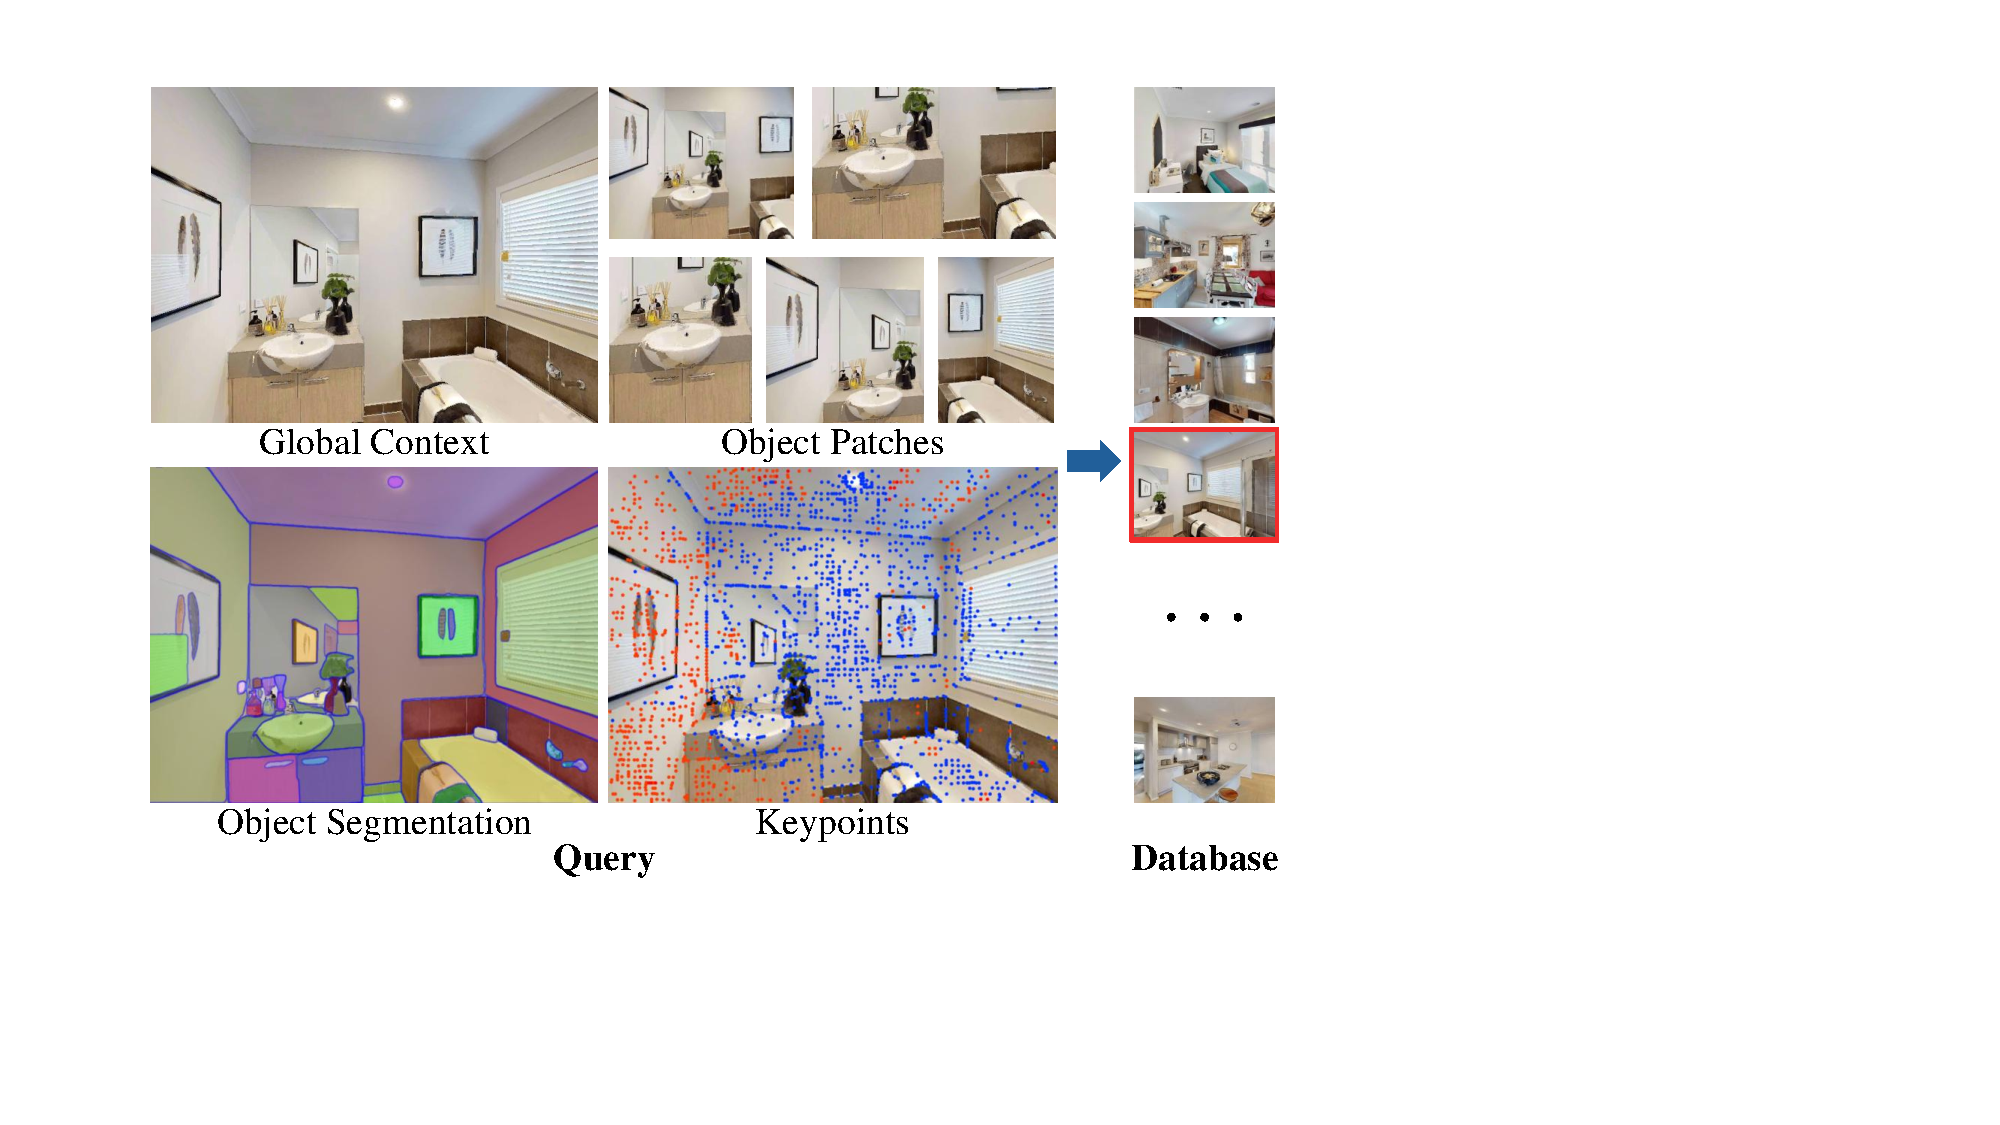
\includegraphics[width=\columnwidth]{object_information_font.pdf}
    \vspace{-20pt}
    \caption{AirRoom leverages multi-level, object-oriented features, including global context, object patches, object segmentation, and keypoints, to perform coarse-to-fine room reidentification.}
    \vspace{-20pt}
    \label{fig:example_image}
\end{figure}

Unlike outdoor environments, where visual place recognition (VPR) methods have matured and perform reliably \cite{arandjelović2016netvladcnnarchitectureweakly, hausler2021patchnetvladmultiscalefusionlocallyglobal, keetha2023anylocuniversalvisualplace}, indoor room ReID remains a challenging problem. A primary reason for this difficulty is the cluttered nature of indoor scenes, which are often densely packed with man-made objects \cite{xu2023clusvprefficientvisualplace}. These densely distributed objects often pose significant challenges to existing methods, which were originally designed for city-style and distinct structures \cite{7339473}. Consequently, these methods struggle to fully capture the intricate details and varied spatial layouts of indoor environments.
% , leading to limitations in their effectiveness when applied to densely populated indoor spaces.
For instance, foundation models like DINO \cite{caron2021emergingpropertiesselfsupervisedvision} and DINOv2 \cite{oquab2024dinov2learningrobustvisual} can generate global descriptors that capture broad scene-level features. However, these descriptors may struggle in semantically similar environments, such as adjacent rooms with similar layouts or decorations, where distinguishable features are minimal \cite{cai2022patchnetvladlearnedpatchdescriptor}. In contrast, methods like Patch-NetVLAD \cite{hausler2021patchnetvladmultiscalefusionlocallyglobal}, AirLoc \cite{aryan2023airlocobjectbasedindoorrelocalization} and AnyLoc \cite{keetha2023anylocuniversalvisualplace} create a global descriptor by aggregating local features, which can enhance discriminative power. Yet, in indoor settings densely populated with similar and repetitive objects, these approaches may still face difficulties in distinguishing between highly similar features, reducing their effectiveness in such contexts \cite{sattler2019understandinglimitationscnnbasedabsolute}.

Additionally, different from room categorization \cite{lee2017roomnetendtoendroomlayout}, which relies on identifying object types to classify spaces into semantic categories, 
%room ReID requires accurately matching specific room instances within a large pre-collected database.
room ReID requires accurately retrieving the same room instance from a reference database based on a given query image. 
For instance, reidentifying a particular kitchen demands a combination of global functional contexts and fine-grained matching of specific object attributes. Moreover, room ReID must handle viewpoint variations, which necessitates tolerance for partial mismatches in object arrangement and appearance. These requirements often result in the failure of algorithms based solely on object categorization, as they lack the precision needed to reidentify unique room instances accurately \cite{Snderhauf2015PlaceRW}.

This raises an important question: \textit{“What kinds of object attributes are truly essential for room ReID?”} To address this, we conduct the first comprehensive study exploring multi-level object-oriented information and its impact on room ReID.
As shown in \fref{fig:example_image}, our experiments show that all four levels of object-oriented information, \ie, global context, object patches, object segmentation, and keypoints, are essential.
Specifically, we find that each level plays a unique role in room ReID. Global context, such as the combination of objects like a couch and television, conveys essential semantic information for categorizing a room as a living room. Object patches provide finer details, enabling differentiation within a room, such as distinguishing a bedside table in a bedroom from a desk in a workspace. Object segmentation offers further granularity by isolating individual items, like separating a dining table from surrounding chairs to clarify the room layout. Finally, keypoints on objects, such as handles on a dresser, enhance room ReID by filtering out visually similar furniture in other rooms. Moreover, integrating multi-level object-oriented information adds robustness to viewpoint variations.

%To address this, we conduct the first comprehensive study that explores the impact of multi-level object information on room ReID. As shown in \fref{fig:example_image}, our experiments demonstrate that all four levels of object information, \textit{i.e.}, global context, object patches, object segmentation, and local keypoints, are essential. Specifically, we find that each level plays a unique role in room ReID. Global context, such as the combination of objects like a couch and television, provides semantic cues to classify a room as a living room. Object patches offer finer detail, helping to distinguish functional zones within a room, such as a sleeping area with a bed and nightstand or a makeup area with a mirror and dressing table in a bedroom. Object segmentation clarifies room layout by isolating specific items, like separating a dining table from surrounding chairs. Finally, local keypoints aid in identifying rooms by filtering out visually similar furniture in other spaces. Moreover, the integration of these four levels of object information significantly improves robustness to viewpoint variations, making our approach adaptable to diverse room perspectives.

% Recent approaches, such as AirLoc \cite{aryan2023airlocobjectbasedindoorrelocalization}, have begun to incorporate object information. However, they rely on pixel-aggregation to form object and room features, which sacrifices critical semantic information, resulting in suboptimal performance. Our findings indicate that objects within indoor environments inherently convey semantic information that aids in room categorization. For example, a combination of objects like a bed, bedside table, and dressing table strongly suggests a bedroom, rather than a kitchen. By incorporating global room representations enriched with object-derived semantics, we achieve broad categorization of rooms. Further, subsets of objects within a room can provide finer details, such as dividing a bedroom into zones like a rest area, with a bed and bedside table, and a makeup area, with a mirror and dressing table. These subsets, or “patches” in image terms, facilitate fine-grained candidate selection. Additionally, individual object details provide further refinement, and local feature matching enhances candidate filtering at an even finer level. Building on these insights, we propose AirRoom—a flexible, object-aware pipeline for room reidentification. AirRoom effectively leverages multi-level object information, boosting reidentification performance while adapting to various configurations, showcasing robustness and versatility across diverse scenarios.

% We find that indoor environments can be broadly categorized into functional types, such as offices, lobbies, and kitchens, each containing distinct semantic information due to the variety of objects present. 
% Global features, rich in appearance and semantic content and extracted from visual backbones, can help select a few functionally similar candidates from a larger pool of irrelevant options \cite{song2022supergfunifyinglocalglobal}. 
% Furthermore, even functionally similar rooms often contain varied objects; for example, different bathrooms may have unique sinks or bathtubs.
% Algorithms that capture this object-level information are generally more effective for achieving accurate and reliable indoor relocalization \cite{qiao2022objectsmatterlearningobject}. 
% Additionally, local feature matching methods, which preserve fine grid information, prove to be highly beneficial \cite{kuang2022densegapgraphstructureddensecorrespondence, wang2024efficientloftrsemidenselocal}. Building on these insights, we propose AirRoom, a novel and flexible object-aware pipeline for indoor relocalization. This approach effectively utilizes object encoding to enhance performance while adapting seamlessly to different module configurations, demonstrating robustness and versatility.
% Recently, methods like AirLoc \cite{aryan2023airlocobjectbasedindoorrelocalization} have attempted to incorporate object information; however, they typically derive object features through a pixel-aggregation approach. This emphasis on local rather than true object-level features has led to limited performance improvements.

% To address these limitations, we pose the question: \textbf{“What if we integrate object encoding into VPR methods?”} We find that indoor environments can be broadly categorized into functional types, such as offices, lobbies, and kitchens, each containing distinct semantic information due to the variety of objects present. Global features, rich in appearance and semantic content and extracted from visual backbones, can help select a few functionally similar candidates from a larger pool of irrelevant options \cite{song2022supergfunifyinglocalglobal}. Furthermore, even functionally similar rooms often contain varied objects; for example, different bathrooms may have unique sinks or bathtubs. Algorithms that capture this object-level information are generally more effective for achieving accurate and reliable indoor relocalization \cite{qiao2022objectsmatterlearningobject}. Additionally, local feature matching methods, which preserve fine grid information, prove to be highly beneficial \cite{kuang2022densegapgraphstructureddensecorrespondence, wang2024efficientloftrsemidenselocal}. Building on these insights, we propose ObjLoc, a novel and flexible object-aware pipeline for indoor relocalization. This approach effectively utilizes object encoding to enhance performance while adapting seamlessly to different module configurations, demonstrating robustness and versatility.
% Recently, methods like AirLoc \cite{aryan2023airlocobjectbasedindoorrelocalization} have attempted to incorporate object information; however, they typically derive object features through a pixel-aggregation approach. This emphasis on local rather than true object-level features has led to limited performance improvements.

Based on these observations, we propose AirRoom, a simple yet highly effective room reidentification (ReID) system consisting of three stages: Global, Local, and Fine-Grained. In the Global stage, a Global Feature Extractor is used to capture global context features, which are then employed to coarsely select five functionally similar candidate rooms. In the Local stage, instance segmentation is applied to identify individual objects, followed by the Receptive Field Expander to extract object patches. An Object Feature Extractor is then used to obtain both object and patch features, which are utilized in Object-Aware Scoring to narrow the selection down to two candidate rooms. Finally, in the Fine-Grained stage, feature matching is employed to precisely identify the final room.

In summary, our contributions include:

\begin{itemize}[leftmargin=2em]
    \item We introduce AirRoom, an object-aware room ReID pipeline with two novel modules: the Receptive Field Expander and Object-Aware Scoring, effectively leveraging multi-level object-oriented information to overcome the limitations observed in previous methods.
    \item We have curated four comprehensive room reidentification datasets—MPReID, HMReID, GibsonReID, and ReplicaReID—providing diverse benchmarks for evaluating room reidentification methods.
    \item Extensive experiments demonstrate that AirRoom outperforms SOTAs, maintaining robust and reliable performance even under significant viewpoint variations.
\end{itemize}

\section{预备知识}

\subsection{定义}

\cpar{原生多模态模型(Native Multimodal Models, NMMs):}
指的是从零开始在所有模态上同时训练的模型,不依赖于预训练的大型语言模型(LLMs)或视觉编码器。我们的关注点是图像和文本这两个典型模态,其中模型同时处理文本和图像作为输入,并生成文本作为输出。

\cpar{早期融合(Early fusion):}
从一开始就实现多模态交互,几乎不使用模态特定的参数(\eg,除了用于图像块化的线性层)。该方法使用一个单一的 transformer 模型,处理原始的多模态 \edit{输入——即标记化的文本和连续的图像块——而无需图像离散化。} \edit{我们}将该主 transformer 称为解码器。

\cpar{晚期融合(Late fusion):}
将多模态交互延后到更深层,通常是在各自的单模态组件 \edit{独立处理完}每个模态之后(\eg,将视觉编码器连接到大型语言模型)。

\cpar{模态无关路由(Modality-agnostic routing):}
在稀疏专家混合机制中,\edit{模态无关}的路由是指依赖于与模型联合训练的学习型路由器模块。

\cpar{模态感知路由(Modality-aware routing):}
基于预定义规则的路由方式,例如根据模态类型进行路由(\eg,视觉 token、文本 token)。

\begin{table}[t!]
    \centering
    \setlength{\tabcolsep}{8pt}
    \renewcommand{\arraystretch}{1.0}
    \resizebox{1\linewidth}{!}{
    \begin{tabular}{c p{0.999\linewidth}}
         Expression & Definition  \\
         \shline
         \textbf{$N$}     & \normalfont{{Number of parameters in the multimodal decoder. For MoEs this refers to the \edit{active parameters.}}} \\
         \grayrow
         \textbf{$D$}     & \normalfont{{Total number of multimodal tokens.}} \\
         \textbf{$N_{v}$} & \normalfont{{Number of vision-only tokens.}} \\
         \grayrow
         \textbf{$D_{v}$} & \normalfont{{Number of parameters in the vision-specific encoder. Only exists in late-fusion architectures.}} \\
         \textbf{$C$}     & \small{{Total number of FLOPs, estimated as $C=6ND$ for early-fusion and $C=6(N_vD_v+ND)$ for late-fusion.}} \\
         \grayrow
         \textbf{$L$}     & \normalfont{{Average validation loss on interleaved image-text, image-caption, and text-only data mixtures.}} \\
    \end{tabular}}
    \caption{本文中使用的表达式的定义。}
    \label{tab:my_label}
\end{table}

\subsection{尺度定律}
我们的目标是理解NMM的尺度特性,以及不同的架构选择如何影响权衡。为此,我们在~\citet{kaplan2020scaling, hoffmann2022training} 提出的尺度定律框架内分析我们的模型。
我们基于总参数数量计算FLOPs,使用近似值 \(C = 6ND\),这一近似在之前的工作中被采用~\citep{hoffmann2022training, abnar2025parameters}。然而,我们对这个估计进行了修改,以适应我们的设置:对于晚期融合模型,FLOPs被计算为 \(6(N_vD_v + ND)\)。
我们考虑一个设置,在给定计算预算 \(C\) 的情况下,我们的目标是预测模型的最终 \edit{损失},并确定最佳的参数数量 \edit{和} 训练令牌数量。与之前关于LLM尺度研究一致~\citep{hoffmann2022training},我们假设最终模型损失与模型大小 (\(N\)) 和训练令牌 (\(D\)) 之间存在幂律关系:

\begin{equation}
\label{eq:scaling_laws}
    L = E + \frac{A}{N^{\alpha}} + \frac{B}{D^{\beta}}.
\end{equation}

\noindent 其中,\(E\) 代表数据集上可实现的最低损失,而 \(\frac{A}{N^{\alpha}}\) 捕捉了增加参数数量的效果,其中更大的模型会导致更低的损失,改善的速度由 \(\alpha\) 控制。类似地,\(\frac{B}{D^{\beta}}\) 反映了更多训练令牌的益处,\(\beta\) 决定了改善的速率。此外,我们假设计算预算(FLOPs)与 \(N\) 和 \(D\) 之间存在线性关系 (\(C \propto ND\))。这进一步导致了在 \cref{tab:power_laws} 中详细描述的幂律关系。

\begin{figure}[t!]
    \centering
    \captionsetup{type=figure}
    \begin{subfigure}[t]{0.48\linewidth}
        \centering
        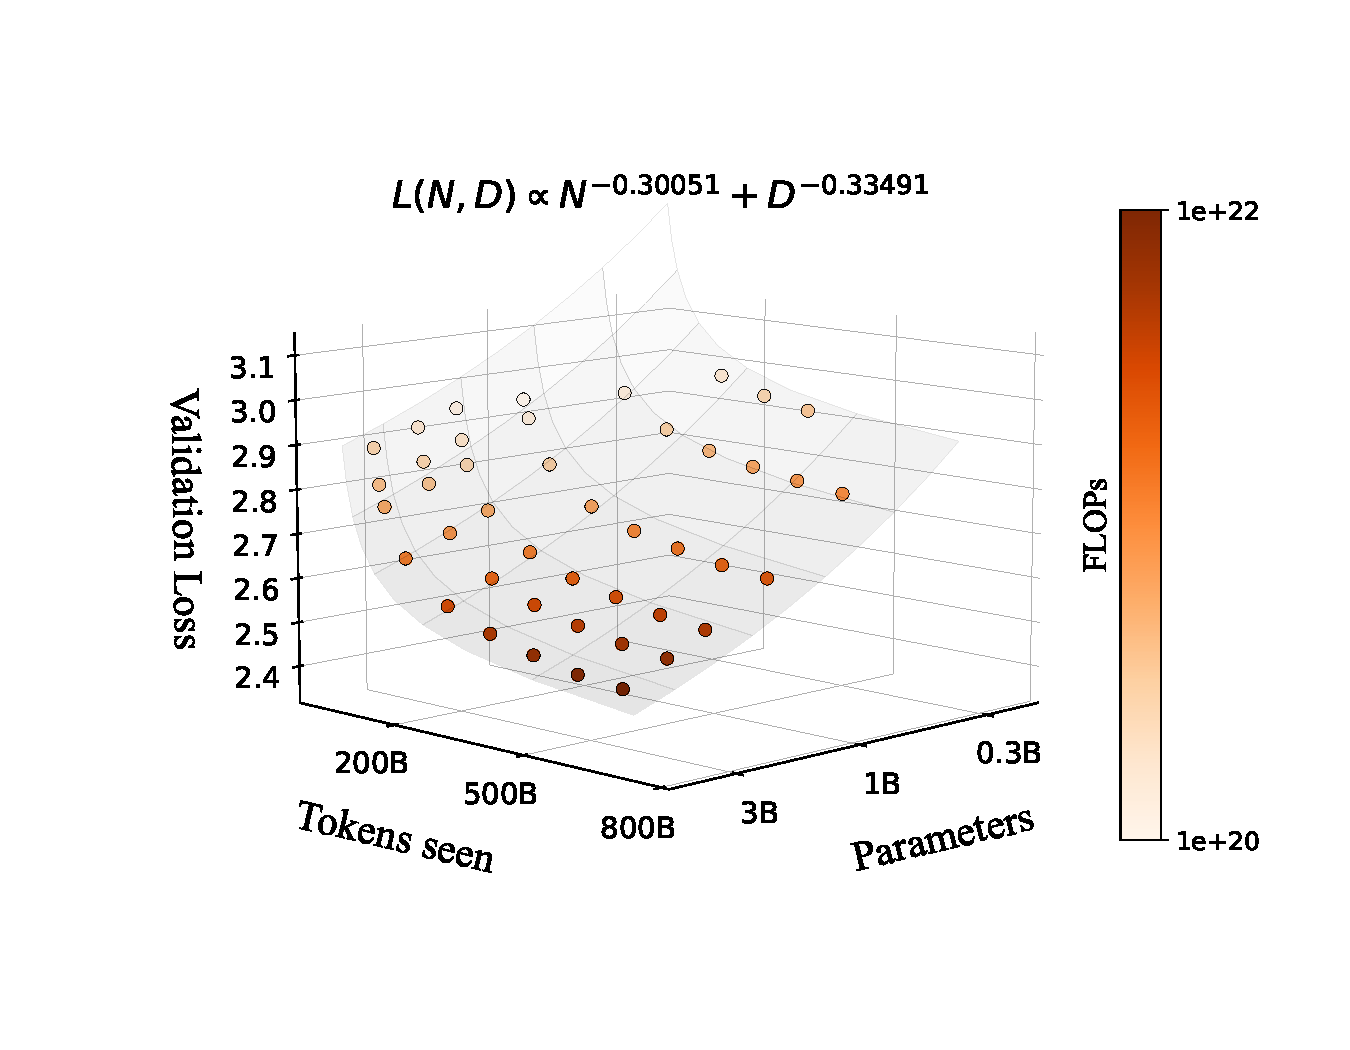
\includegraphics[width=1.02\linewidth]{assets/early/3d_scaling_early.pdf}
    \end{subfigure}
    \hfil
    \begin{subfigure}[t]{0.48\linewidth}
        \centering
        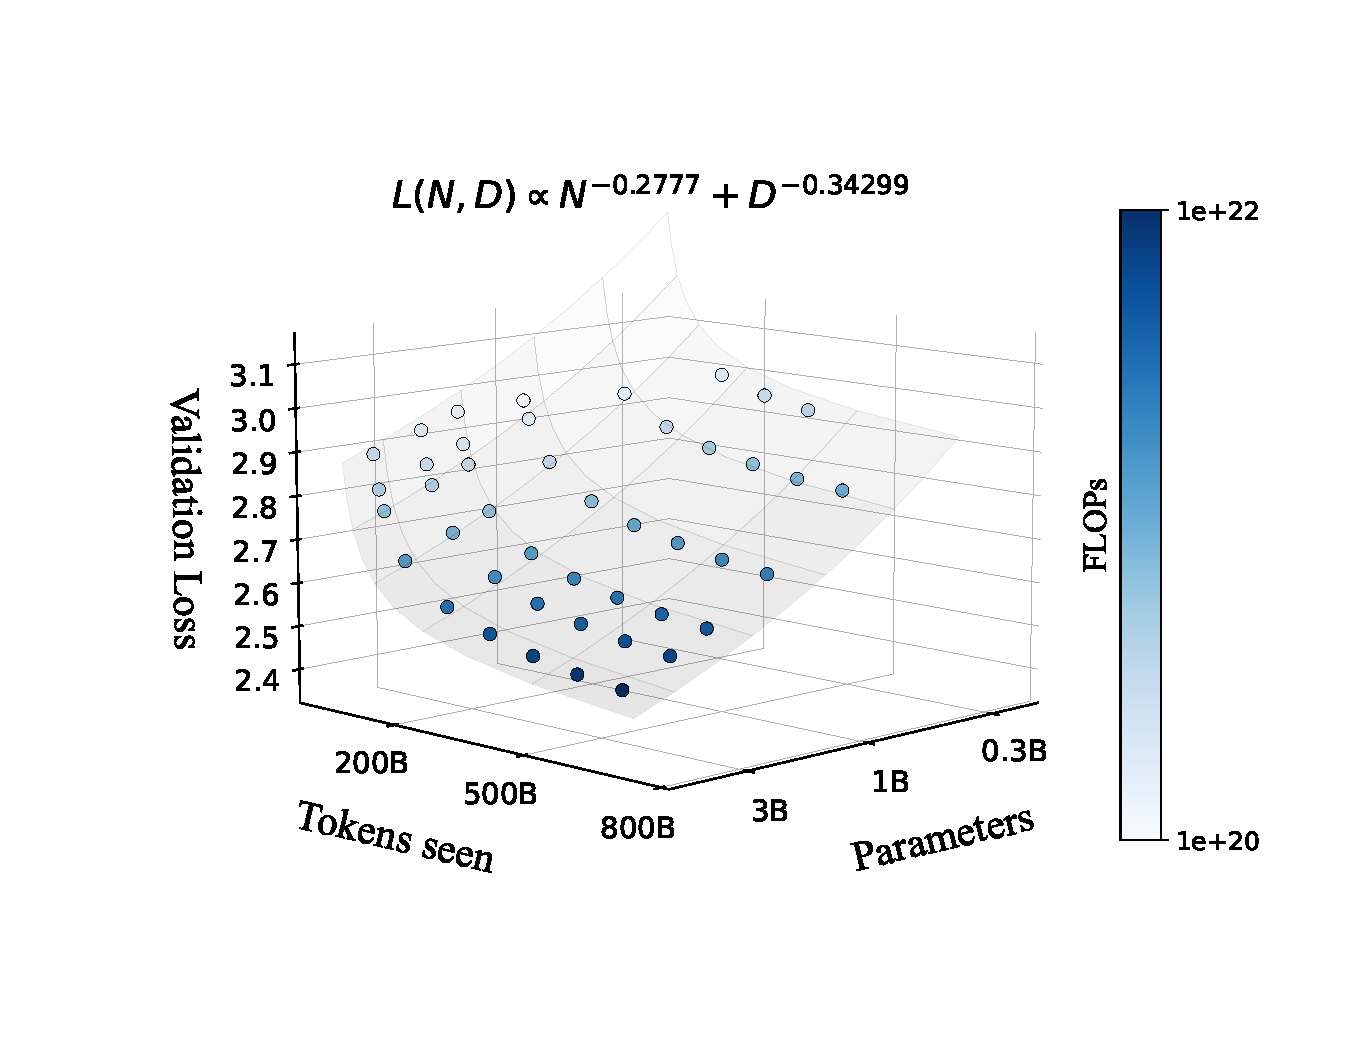
\includegraphics[width=1.02\linewidth]{assets/early/3d_scaling_late.pdf}
    \end{subfigure}
    \vspace{5pt}
    \setlength{\fboxsep}{0.5pt}
    \setlength{\fboxrule}{0pt}
    \caption{\textbf{原生多模态模型中 \fbox{\colorbox{CustomC_Light1!20}{\strut early-fusion}} 与 \fbox{\colorbox{CustomD_Light1!20}{late-fusion\strut}} 的尺度规律。} 每个点表示一个在不同 \edit{数量的} tokens(250M 到 400B)上训练的模型(300M 到 3B 参数)。我们报告了在 \edit{交错数据(Obelics)、图像描述数据(HQITP)和纯文本数据(DCLM)} 的验证集上的平均交叉熵损失。}
    \label{fig:early_vs_late_scaleflops_3d}
\end{figure}


\begin{table}[h]
    \centering
    \setlength{\tabcolsep}{16pt}
    \renewcommand{\arraystretch}{1}
    \resizebox{1\linewidth}{!}{
    \begin{tabular}{lccrc}
        Data type & dataset & \#samples & sampling prob. \\
         \shline
         \multirow{3}{*}{Image-Caption} &  DFN~\citep{fang2023data} & 2B & 27\%
         \\
          & COYO~{\citep{kakaobrain2022coyo700m}} &  600M & 11.25\% \\
          & HQITP  & 400M & 6.75\% \\
          Interleaved & Obelics \citep{laurenccon2024obelics}  & 141M Docs &
          45\% \\
          Text & DCLM \citep{li2024datacomp} & 6.6T Toks & 10\% \\

    \end{tabular}} \caption{\textbf{预训练数据混合。} 除非另有说明,训练混合数据包含45\%、45\%和10\%的图像说明、交错文档和仅文本数据。}
    \label{tab:pretraining_datasets}
    \vspace{-5pt}
\end{table}
\subsection{实验设置}
\edit{我们的模型}基于自回归Transformer架构~\citep{vaswani2017attention},采用SwiGLU FFNs~\citep{shazeer2020glu}和QK-Norm~\citep{dehghani2023scaling},参照~\citet{li2024datacomp}的方法。在早期融合模型中,图像块被线性映射到与文本标记维度匹配,而晚期融合则遵循CLIP架构~\citep{radford2021learning}。我们为文本标记采用因果注意力,为图像标记采用双向注意力,发现这种方式效果更佳。训练是在混合的公共和私有多模态数据集上进行的,包括DCLM \citep{li2024datacomp}、Obelics \citep{laurenccon2024obelics}、DFN \citep{fang2023data}、COYO \citep{kakaobrain2022coyo700m},以及一个私有的高质量图像-文本对(HQITP)集合(见\cref{tab:pretraining_datasets})。图像被\edit{调整大小}为224×224分辨率,图像块大小为14×14。我们为多模态序列采用1k的上下文长度。为了提高训练效率,我们使用\texttt{bfloat16}、完全分片数据并行(FSDP)\citep{zhao2023pytorch}、\edit{激活}检查点和梯度累积进行训练。我们还对图像字幕数据集使用序列打包,以减少填充标记的数量。与之前的工作~\citep{hoffmann2022training,aghajanyan2023scalingmm,abnar2025parameters}类似,我们在交替(Obelics)、图像-字幕(HQITP)和仅文本数据(DCLM)上评估性能。更多实现细节请参见~\cref{app:implementation_details}。







 











\section{Scaling  native multimodal models}








In this section, we present a scaling laws study of native multimodal models,
examining various architectural choices~\cref{sec:scaling_laws_early}, exploring
different data mixtures~\cref{sec:scaling_data_mix}, analyzing the practical
trade-offs between late and early fusion
NMMs, and comparing the performance of native
pre-training and continual pre-training of NMMs~\cref{sec:native_vs_continual}.  

\cpar{Setup.} We train models ranging from 0.3B to 4B active parameters,
scaling the width while keeping the depth constant. For smaller training token
budgets, we reduce the warm-up phase to 1K steps while maintaining 5K steps for
larger budgets.  
Following~\citet{hagele2024scaling}, models are trained with a constant learning
rate, followed by a cool-down phase using an inverse square root scheduler. The
cool-down phase spans 20\% of the total steps spent at the constant learning
rate.  To estimate the scaling coefficients in \Cref{eq:scaling_laws}, we apply the
L-BFGS algorithm~\citep{lbfgs} and Huber loss~\citep{Huber1992} (with $\delta =
10^{-3}$), performing a grid search over initialization ranges.  







\begin{table}[h!]
    \begin{minipage}[b]{1\linewidth}
        \centering
        \setlength{\tabcolsep}{24pt}
        \renewcommand{\arraystretch}{1}
        \resizebox{1\linewidth}{!}{
        \begin{tabular}{c c c c c}
             \grayrow $L \propto E+\frac{1}{N^{\alpha}}+\frac{1}{D^{\beta}}$ & $N \propto C^a$ & $D \propto C^b$ & $L \propto C^c$ & $D \propto N^d$ \\
        \end{tabular}}
      \label{tab:power_laws}
      \vspace{-3mm}
    \end{minipage}
    \begin{minipage}[b]{1\linewidth}
        \centering
        \setlength{\tabcolsep}{8pt}
        \renewcommand{\arraystretch}{1}
        \resizebox{1\linewidth}{!}{
        \begin{tabular}{lccccccccc}
            Model & Data & E & $\alpha$ & $\beta$ & a & b  & c & d \\ %
            \shline
            GPT3 \citep{brown2020language} & Text &  -- & -- & -- & -- & -- & -0.048 & \\% & 1.7 \\
            Chinchilla \citep{hoffmann2022training} & Text &  1.693 & 0.339 & 0.285 & 0.46 & 0.54 & -- & \\%& 20 \\
            \midrule
            \multirow{4}{*}{NMM (early-fusion)} & Text &  2.222 & 0.308 & 0.338 & 0.525 & 0.477     & -0.042 & 0.909 \\%& 58.35\\
            & Image-Caption & 1.569 & 0.311 & 0.339 & 0.520 & 0.479 & -0.061 & 0.919 \\% & 72.21\\
            & Interleaved & 1.966 & 0.297 & 0.338 & 0.532 & 0.468     & -0.046 & 0.879 \\%& 57.74\\
            & AVG & 1.904 & 0.301 & 0.335 & 0.526 & 0.473 & -0.049 & 0.899 \\% & 64.05\\
            \midrule
            NMM (late-fusion) & AVG &  1.891 & 0.290 & 0.338 & 0.636 & 0.462 & -0.049 & 0.673 \\%& 46.19\\
            \midrule
            \edit{Sparse NMM (early-fusion)} & AVG & 2.158  & 0.710 & 0.372 & 0.361  & 0.656 & -0.047 & 1.797 \\%& 46.19\\
        \end{tabular}%
        } \caption{\textbf{Scaling laws for native multimodal models}. We report the
        scaling laws results for early and late fusion models. We fit the scaling laws for different target data types as well as their average loss (AVG).
        }
        \label{tab:early_vs_late_coeffs}
    \end{minipage}
    \vspace{-3mm}
\end{table}
       

\begin{figure*}[t!]
    \centering
    \captionsetup{type=figure}
    \begin{subfigure}[t]{0.33\linewidth}
        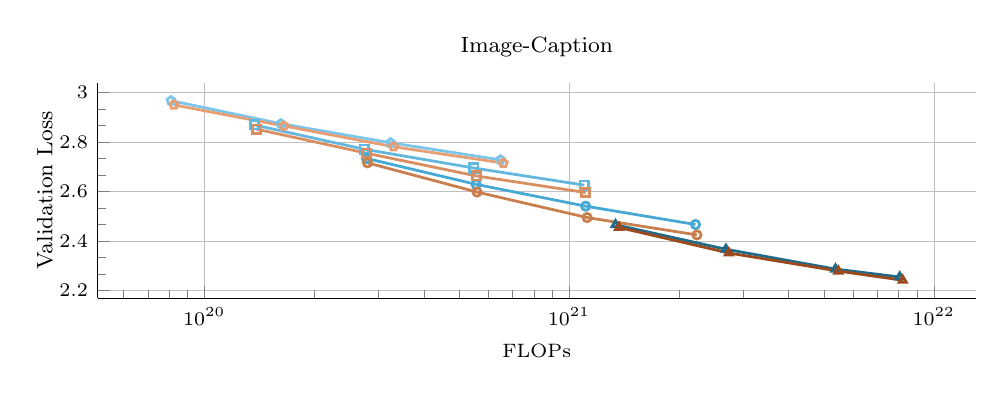
\begin{tikzpicture}
    \begin{axis}[
        legend pos=north east,
        grid=major, %
        grid style={line width=.1pt, draw=gray!30}, %
        major grid style={line width=.2pt,draw=gray!50},
        minor tick num=2,
        axis x line*=bottom,
        axis y line*=left,
        xmode=log, %
        log basis x=10, %
        height=1.7in,
        width=1.05\linewidth,
        ylabel style={align=center, font=\scriptsize, yshift=-1ex},
        xlabel style={font=\scriptsize},
        ylabel={\footnotesize{Validation Loss}},
        xlabel={\scriptsize{FLOPs}},
        title=\footnotesize{Image-Caption},
        yticklabel style={font=\scriptsize, /pgf/number format/fixed, /pgf/number format/precision=1},
        xticklabel style={font=\scriptsize},
        mark options={solid},
        legend style={cells={align=left}, font=\footnotesize, text=black}, %
        legend columns=6, %
        legend cell align={left},
        legend to name=sharedlegend,
    ]
    \addplot[legend late_0_2b style] plot coordinates {
        (8.1e+19, 2.967)
        (1.62e+20, 2.874)
        (3.24e+20, 2.797)
        (6.48e+20, 2.728)

    };

    \addplot[legend late_0_4b style] plot coordinates {
        (1.37e+20, 2.869)
        (2.74e+20, 2.771)
        (5.48e+20, 2.695)
        (1.1e+21, 2.626)

    };

    \addplot[legend late_0_9b style] plot coordinates {
        (2.78e+20, 2.734)
        (5.56e+20, 2.629)
        (1.11e+21, 2.541)
        (2.22e+21, 2.467)

    };



    \addplot[legend late_2_2b style] plot coordinates {
        (1.34e+21, 2.466)
        (2.69e+21, 2.367)
        (5.37e+21, 2.287)
        (8.06e+21, 2.255)
    };

        







    \addplot[legend early_0_2b style] plot coordinates {
        (8.25e+19, 2.95)
        (1.65e+20, 2.865)
        (3.3e+20, 2.781)
        (6.6e+20, 2.715)


    };
    \addplot[legend early_0_4b style] plot coordinates {
        (1.39e+20, 2.852)
        (2.78e+20, 2.755)
        (5.57e+20, 2.663)
        (1.11e+21, 2.596)


    };
    \addplot[legend early_0_9b style] plot coordinates {
        (2.8e+20, 2.716)
        (5.59e+20, 2.598)
        (1.12e+21, 2.495)
        (2.24e+21, 2.425)


    };

        
    \addplot[legend early_2_2b style] plot coordinates {
        (1.37e+21, 2.455)
        (2.74e+21, 2.352)
        (5.47e+21, 2.279)
        (8.21e+21, 2.242)
    };
        
    

    \end{axis}
\end{tikzpicture}
    \end{subfigure}
    \begin{subfigure}[t]{0.32\linewidth}
        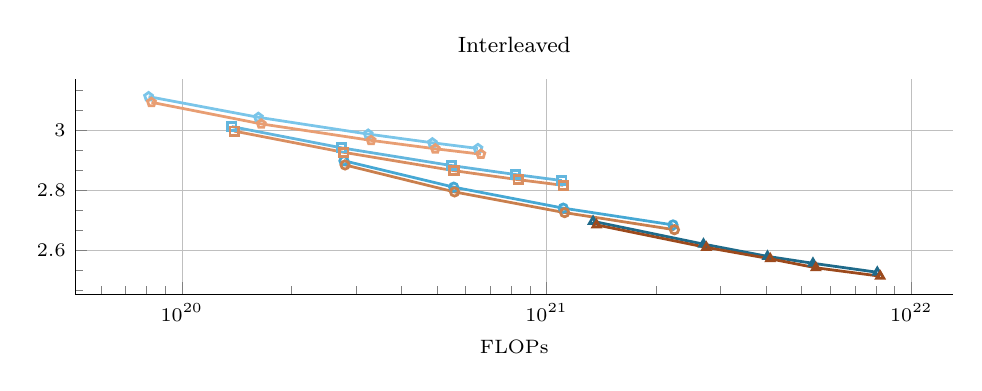
\begin{tikzpicture}
    \begin{axis}[
        legend pos=north east,
        grid=major,
        grid style={line width=.1pt, draw=gray!30},
        major grid style={line width=.2pt,draw=gray!50},
        minor tick num=2,
        axis x line*=bottom,
        axis y line*=left,
        xmode=log,
        log basis x=10,
        height=1.7in,
        width=1.05\linewidth,
        ylabel style={align=center, font=\scriptsize, yshift=-1ex},
        xlabel style={font=\scriptsize},
        xlabel={\scriptsize{FLOPs}},
        title=\footnotesize{Interleaved},
        yticklabel style={font=\scriptsize, /pgf/number format/fixed, /pgf/number format/precision=1},
        xticklabel style={font=\scriptsize},
        mark options={solid},
        legend style={cells={align=left}, font=\footnotesize, text=black},
        legend columns=6,
        legend cell align={left},
        legend to name=sharedlegend,
    ]

\addplot[legend late_0_2b style] plot coordinates {
        (8.1e+19, 3.113)
        (1.62e+20, 3.044)
        (3.24e+20, 2.988)
        (4.86e+20, 2.959)
        (6.48e+20, 2.94)
    };

    \addplot[legend late_0_4b style] plot coordinates {
        (1.37e+20, 3.013)
        (2.74e+20, 2.942)
        (5.48e+20, 2.883)
        (8.22e+20, 2.853)
        (1.1e+21, 2.833)

    };

    \addplot[legend late_0_9b style] plot coordinates {
        (2.78e+20, 2.899)
        (5.56e+20, 2.811)
        (1.11e+21, 2.741)
        (2.22e+21, 2.685)

    };
    \addlegendentry{Late-1B}

\addplot[legend late_2_2b style] plot coordinates {
        (1.34e+21, 2.697)
        (2.69e+21, 2.621)
        (4.03e+21, 2.58)
        (5.37e+21, 2.557)
        (8.06e+21, 2.527)

    };
    \addlegendentry{Late-2.4B}

\addplot[legend early_0_2b style] plot coordinates {
        (8.25e+19, 3.094)
        (1.65e+20, 3.022)
        (3.3e+20, 2.967)
        (4.95e+20, 2.939)
        (6.6e+20, 2.921)
    };

    \addplot[legend early_0_4b style] plot coordinates {
        (1.39e+20, 2.998)
        (2.78e+20, 2.927)
        (5.57e+20, 2.866)
        (8.35e+20, 2.836)
        (1.11e+21, 2.817)
    };

    \addplot[legend early_0_9b style] plot coordinates {
        (2.8e+20, 2.885)
        (5.59e+20, 2.795)
        (1.12e+21, 2.726)
        (2.24e+21, 2.669)
    };

    \addlegendentry{Early-0.9B}

\addplot[legend early_2_2b style] plot coordinates {
        (1.37e+21, 2.685)
        (2.74e+21, 2.61)
        (4.1e+21, 2.572)
        (5.47e+21, 2.542)
        (8.21e+21, 2.514)

    };
    \addlegendentry{Early-2.2B}

\end{axis}
\end{tikzpicture}

    \end{subfigure}
    \begin{subfigure}[t]{0.32\linewidth}
    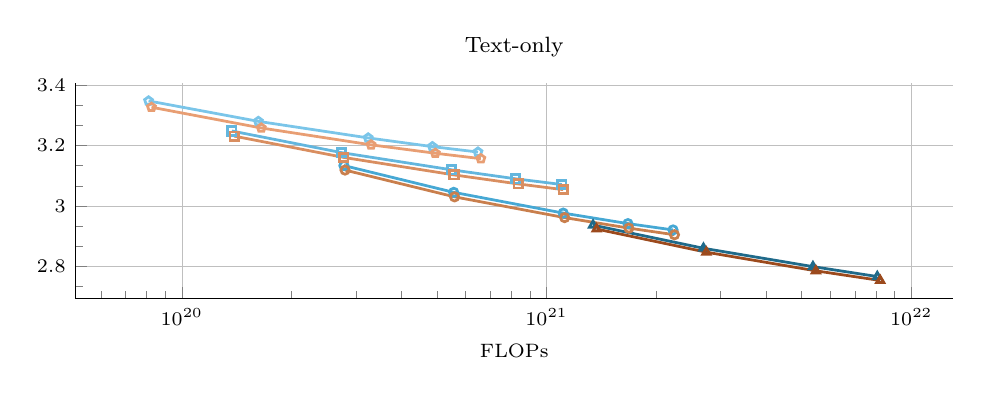
\begin{tikzpicture}
    \begin{axis}[
        legend pos=north east,
        grid=major,
        grid style={line width=.1pt, draw=gray!30},
        major grid style={line width=.2pt,draw=gray!50},
        minor tick num=2,
        axis x line*=bottom,
        axis y line*=left,
        xmode=log,
        log basis x=10,
        height=1.7in,
        width=1.05\linewidth,
        ylabel style={align=center, font=\scriptsize, yshift=-1ex},
        xlabel style={font=\scriptsize},
        xlabel={\scriptsize{FLOPs}},
        title=\footnotesize{Text-only},
        yticklabel style={font=\scriptsize, /pgf/number format/fixed, /pgf/number format/precision=1},
        xticklabel style={font=\scriptsize},
        mark options={solid},
        legend style={cells={align=left}, font=\scriptsize, text=black},
        legend columns=4,
        legend cell align={left},
        legend to name=sharedlegend,
    ]

    \addplot[legend late_0_2b style] plot coordinates {
        (8.1e+19, 3.349)
        (1.62e+20, 3.281)
        (3.24e+20, 3.226)
        (4.86e+20, 3.197)
        (6.48e+20, 3.179)

    };
    \addlegendentry{Late-289M}

    \addplot[legend late_0_4b style] plot coordinates {
        (1.37e+20, 3.249)
        (2.74e+20, 3.177)
        (5.48e+20, 3.12)
        (8.22e+20, 3.09)
        (1.1e+21, 3.071)
    };
    \addlegendentry{Late-494M}

\addplot[legend late_0_9b style] plot coordinates {
        (2.78e+20, 3.134)
        (5.56e+20, 3.045)
        (1.11e+21, 2.976)
        (1.67e+21, 2.941)
        (2.22e+21, 2.92)

    };
    \addlegendentry{Late-1B}

\addplot[legend late_2_2b style] plot coordinates {
        (1.34e+21, 2.936)
        (2.69e+21, 2.859)
        (5.37e+21, 2.798)
        (8.06e+21, 2.765)

    };
    \addlegendentry{Late-2.4B}

\addplot[legend early_0_2b style] plot coordinates {
        (8.25e+19, 3.328)
        (1.65e+20, 3.259)
        (3.3e+20, 3.203)
        (4.95e+20, 3.175)
        (6.6e+20, 3.157)
    };
    \addlegendentry{Early-275M}

\addplot[legend early_0_4b style] plot coordinates {
        (1.39e+20, 3.232)
        (2.78e+20, 3.161)
        (5.57e+20, 3.103)
        (8.35e+20, 3.073)
        (1.11e+21, 3.054)
    };
    \addlegendentry{Early-464M}

    \addplot[legend early_0_9b style] plot coordinates {
        (2.8e+20, 3.119)
        (5.59e+20, 3.03)
        (1.12e+21, 2.961)
        (1.68e+21, 2.926)
        (2.24e+21, 2.904)
    };
    \addlegendentry{Early-932M}

\addplot[legend early_2_2b style] plot coordinates {
        (1.37e+21, 2.923)
        (2.74e+21, 2.846)
        (5.47e+21, 2.784)
        (8.21e+21, 2.752)
    };
    \addlegendentry{Early-2.28B}

\end{axis}
\end{tikzpicture}

    \end{subfigure}
    \begin{center}
        \ref{sharedlegend}
    \end{center}
    \caption{\textbf{早期融合与晚期融合:缩放训练浮点运算。} 我们比较了在缩放模型参数数量和训练词元数量时的早期融合模型和晚期融合模型。总体而言,早期融合显示出轻微的优势,尤其是在较小的模型规模下,随着参数数量的增加,差距减小 $N$ 。}
    \label{fig:early_vs_late_scaleflops}
    \vspace{3mm}
\end{figure*}




\vspace{-0.5cm}
\subsection{Scaling laws of NMMs}
\label{sec:scaling_laws_early}

\cpar{Scaling laws for early-fusion and late-fusion models.}  
\Cref{fig:early_vs_late_scaleflops_3d}~(left) presents the final loss averaged
across interleaved, image-caption, and text datasets for early-fusion NMMs. The
lowest-loss frontier follows a power law as a function of FLOPs. Fitting the
power law yields the expression $L \propto C^{-0.049}$, indicating the rate of
improvement with increasing compute. When analyzing the scaling laws per data
type (\eg, image-caption, interleaved, text), we observe that the exponent
varies (\cref{tab:early_vs_late_coeffs}). For instance, the model achieves a
higher rate of improvement for image-caption data $(L \propto C^{-0.061})$ when
compared to interleaved documents $(L \propto C^{-0.046}$).  

To model the loss as a function of the number of training tokens $D$ and model
parameters $N$, we fit the parametric function in \cref{eq:scaling_laws}, obtaining
scaling exponents $\alpha = 0.301$ and $\beta = 0.335$. These describe the rates
of improvement when scaling the number of model parameters and training tokens, respectively.
Assuming a linear relationship between compute, $N$, and $D$ (\ie, $C \propto ND$),
we derive the law relating model parameters to the compute budget (see
\cref{app:scaling_laws} for details). Specifically, for a given compute budget
$C$, we compute the corresponding model size $N$ at logarithmically spaced $D$
values and determine $N_{opt}$, the parameter count that minimizes loss.
Repeating this across different FLOPs values produces a dataset of $(C,
N_{opt})$, to which we fit a power law predicting the compute-optimal model size
as a function of compute: $N^* \propto C^{0.526}.$

Similarly, we fit power laws to estimate the compute-optimal training dataset
size as a function of compute and model size:  
\[
D_{opt} \propto C^{0.473}, \quad D_{opt} \propto N^{0.899}.
\]  
These relationships allow practitioners to determine the optimal model and
dataset size given a fixed compute budget. When analyzing by data type, we find
that interleaved data benefits more from larger models ($a=0.532$) compared to
image-caption data ($a=0.520$), whereas the opposite trend holds for training
tokens.  





\begin{figure*}[t!]
    \centering
    \captionsetup{type=figure}
    \begin{subfigure}[t]{0.24\linewidth}
        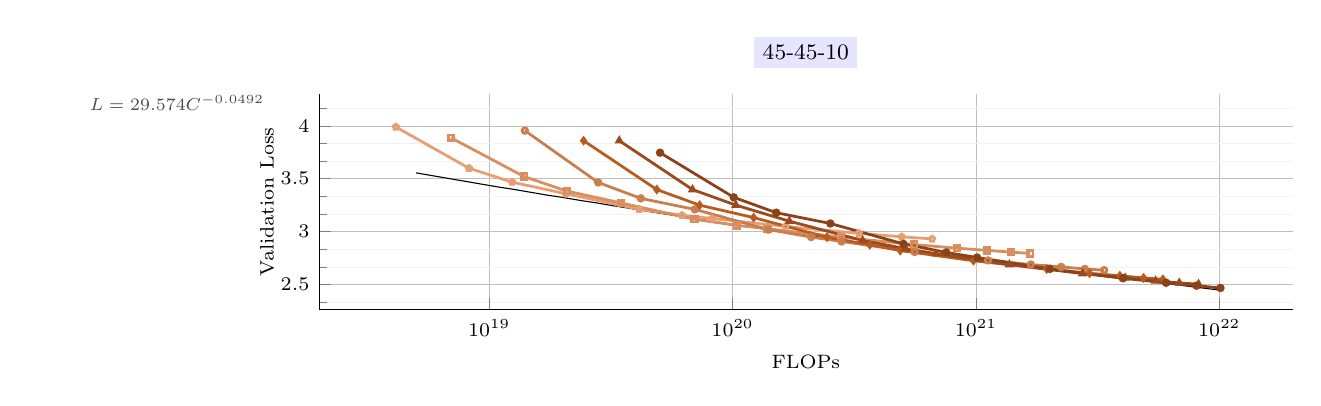
\begin{tikzpicture}
    \begin{axis}[
        grid=both,
        grid style={line width=.1pt, draw=gray!10},
        major grid style={line width=.2pt,draw=gray!50},
        minor tick num=2,
        axis x line*=bottom,
        axis y line*=left,
        xmode=log,
        log basis x=10,
        xtick={
            1E+19,
            1E+20,
            1E+21,
            1E+22
        },
        xmin=2E+18,
        xmax=2E+22,
        ymax=4.3,
        height=1.7in,
        width=1.15\linewidth,
        ylabel style={align=center, font=\scriptsize, yshift=-1ex},
        xlabel style={font=\scriptsize},
        title={\footnotesize{\colorbox{blue!10}{45-45-10}}},
        ylabel={Validation Loss},
        xlabel={\scriptsize{FLOPs}},
        yticklabel style={font=\scriptsize},
        xticklabel style={font=\scriptsize},
        legend style={cells={align=left}, font=\scriptsize, fill opacity=0.7, fill=none,at={(-0.3,0.95)}, anchor=west, draw=none},
        legend cell align={left},
        mark options={solid},
    ]

\addplot[color=white, samples=50, domain=5e18:10e21, mark=none] {29.574*x^(-0.04919)};
    \addlegendentry{\scalebox{0.9}{$L = 29.574C^{-0.0492}$}};
    \addplot[color=black, samples=50, domain=5e18:10e21, forget plot] {29.574*x^(-0.04919)};

\addplot[legend early_0_2b style, mark size=1pt] plot coordinates {
        (4.13e+18, 3.9896666666666665)
        (8.25e+18, 3.5996666666666663)
        (1.24e+19, 3.468)
        (2.06e+19, 3.358333333333333)
        (4.13e+19, 3.2113333333333336)
        (6.19e+19, 3.1543333333333337)
        (8.25e+19, 3.124)
        (1.65e+20, 3.048666666666667)
        (3.3e+20, 2.9836666666666667)
        (4.95e+20, 2.9506666666666668)
        (6.6e+20, 2.9309999999999996)
    };
    \addplot[legend early_0_4b style, mark size=1pt] plot coordinates {
        (6.96e+18, 3.887333333333333)
        (1.39e+19, 3.5203333333333333)
        (2.09e+19, 3.3823333333333334)
        (3.48e+19, 3.2710000000000004)
        (6.96e+19, 3.1170000000000004)
        (1.04e+20, 3.058666666666667)
        (1.39e+20, 3.0273333333333334)
        (2.78e+20, 2.9476666666666667)
        (5.57e+20, 2.877333333333333)
        (8.35e+20, 2.8433333333333333)
        (1.11e+21, 2.8223333333333334)
        (1.39e+21, 2.8063333333333333)
        (1.67e+21, 2.7936666666666667)
    };
    \addplot[legend early_0_9b style, mark size=1pt] plot coordinates {
        (1.4e+19, 3.955)
        (2.8e+19, 3.465)
        (4.19e+19, 3.3143333333333334)
        (6.99e+19, 3.2099999999999995)
        (1.4e+20, 3.0193333333333334)
        (2.1e+20, 2.9483333333333337)
        (2.8e+20, 2.9066666666666663)
        (5.59e+20, 2.807666666666666)
        (1.12e+21, 2.7273333333333327)
        (1.68e+21, 2.688333333333333)
        (2.24e+21, 2.666)
        (2.8e+21, 2.6466666666666665)
        (3.36e+21, 2.635333333333333)
    };

    \addplot[legend early style, mark size=1pt] plot coordinates {
        (2.44e+19, 3.859666666666667)
        (4.88e+19, 3.3973333333333335)
        (7.32e+19, 3.25)
        (1.22e+20, 3.1323333333333334)
        (2.44e+20, 2.9466666666666668)
        (3.66e+20, 2.875666666666667)
        (4.88e+20, 2.8206666666666664)
        (9.76e+20, 2.7246666666666672)
        (1.95e+21, 2.646666666666667)
        (2.93e+21, 2.6056666666666666)
        (3.9e+21, 2.582333333333333)
        (4.88e+21, 2.562)
        (5.86e+21, 2.548666666666666)
    };

    \addplot[legend early_2_2b style, mark size=1pt] plot coordinates {
        (3.42e+19, 3.859666666666667)
        (6.84e+19, 3.3973333333333335)
        (1.03e+20, 3.2503333333333333)
        (1.71e+20, 3.098333333333333)
        (3.42e+20, 2.9156666666666666)
        (5.13e+20, 2.8396666666666666)
        (6.84e+20, 2.7913333333333337)
        (1.37e+21, 2.687666666666667)
        (2.74e+21, 2.6026666666666665)
        (4.1e+21, 2.562)
        (5.47e+21, 2.5349999999999997)
        (6.84e+21, 2.5146666666666664)
        (8.21e+21, 2.502666666666667)
    };
    \addplot[legend early_3_3b style, mark size=1pt] plot coordinates {
        (5.03e+19, 3.746333333333333)
        (1.01e+20, 3.324)
        (1.51e+20, 3.1786666666666665)
        (2.52e+20, 3.0766666666666667)
        (5.03e+20, 2.8836666666666666)
        (7.55e+20, 2.8029999999999995)
        (1.01e+21, 2.7550000000000003)
        (2.01e+21, 2.6473333333333335)
        (4.02e+21, 2.5583333333333336)
        (6.04e+21, 2.5163333333333333)
        (8.05e+21, 2.4886666666666666)
        (1.01e+22, 2.466666666666667)
    };

\end{axis}
\end{tikzpicture}

    \end{subfigure}
    \begin{subfigure}[t]{0.24\linewidth}
        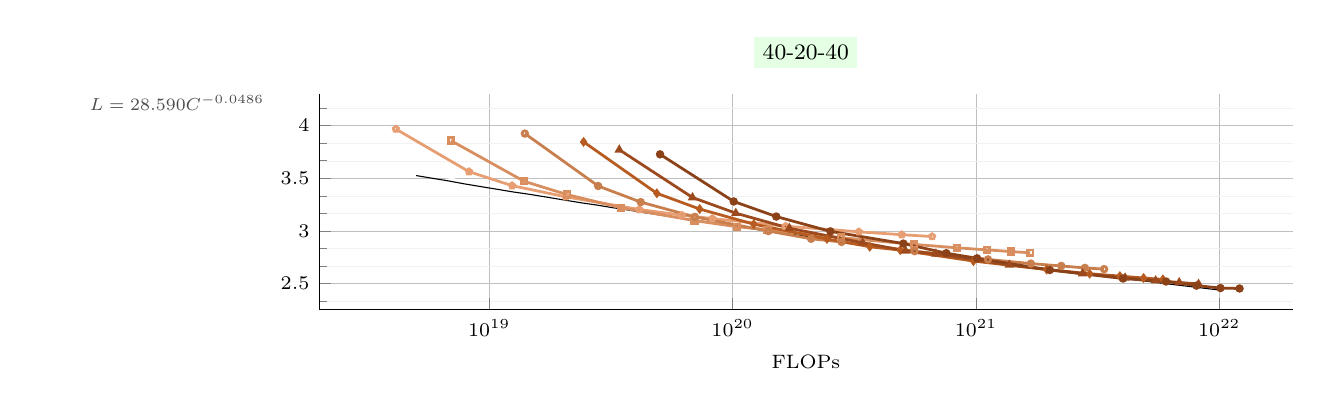
\begin{tikzpicture}
    \begin{axis}[
        legend pos=north east,
        grid=both,
        grid style={line width=.1pt, draw=gray!10},
        major grid style={line width=.2pt,draw=gray!50},
        minor tick num=2,
        axis x line*=bottom,
        axis y line*=left,
        xmode=log,
        log basis x=10,
        xtick={
            1E+19,
            1E+20,
            1E+21,
            1E+22
        },
        xmin=2E+18,
        xmax=2E+22,
        ymax=4.3,
        height=1.7in,
        width=1.15\linewidth,
        ylabel style={align=center, font=\scriptsize, yshift=-1ex},
        xlabel style={font=\scriptsize},
        title=\footnotesize{\colorbox{green!10}{40-20-40}},
        xlabel={\scriptsize{FLOPs}},
        yticklabel style={font=\scriptsize},
        xticklabel style={font=\scriptsize},
        legend style={cells={align=left}, font=\scriptsize, fill opacity=0.7, fill=none,  draw=none,at={(-0.3,0.95)}, anchor=west},
        legend cell align={left},
        mark options={solid},
    ]

    \addplot[color=white, samples=50, domain=5e18:10e21, mark=none] {29.574*x^(-0.04919)};
    \addlegendentry{\scalebox{0.9}{$L = 28.590C^{-0.0486}$}};
    \addplot[color=black, samples=50, domain=5e18:10e21] {28.589490029895153*x^(-0.048605069004824725)};

    \addplot[legend early_0_2b style, mark size=1pt] plot coordinates {
        (4.13e+18, 3.968)
        (8.25e+18, 3.563)
        (1.24e+19, 3.4296666666666664)
        (2.06e+19, 3.3236666666666665)
        (4.13e+19, 3.203)
        (6.19e+19, 3.1486666666666667)
        (8.25e+19, 3.1169999999999995)
        (1.65e+20, 3.0446666666666666)
        (3.3e+20, 2.9906666666666673)
        (4.95e+20, 2.9633333333333334)
        (6.6e+20, 2.9456666666666664)
    };
    \addplot[legend early_0_4b style, mark size=1pt] plot coordinates {
        (6.96e+18, 3.8580000000000005)
        (1.39e+19, 3.471)
        (2.09e+19, 3.3443333333333336)
        (3.48e+19, 3.2196666666666665)
        (6.96e+19, 3.097666666666667)
        (1.04e+20, 3.0393333333333334)
        (1.39e+20, 3.011333333333333)
        (2.78e+20, 2.935333333333333)
        (5.57e+20, 2.871)
        (8.35e+20, 2.8386666666666667)
        (1.11e+21, 2.8190000000000004)
        (1.39e+21, 2.8030000000000004)
        (1.67e+21, 2.7913333333333337)
    };
    \addplot[legend early_0_9b style, mark size=1pt] plot coordinates {
        (1.4e+19, 3.9250000000000003)
        (2.8e+19, 3.426666666666667)
        (4.19e+19, 3.2733333333333334)
        (6.99e+19, 3.1326666666666667)
        (1.4e+20, 2.9979999999999998)
        (2.1e+20, 2.9246666666666665)
        (2.8e+20, 2.8943333333333334)
        (5.59e+20, 2.8070000000000004)
        (1.12e+21, 2.7283333333333335)
        (1.68e+21, 2.6886666666666668)
        (2.24e+21, 2.666)
        (2.8e+21, 2.6476666666666664)
        (3.36e+21, 2.636)
    };

    \addplot[legend early style, mark size=1pt] plot coordinates {
        (2.44e+19, 3.846)
        (4.88e+19, 3.3570000000000007)
        (7.32e+19, 3.207333333333333)
        (1.22e+20, 3.0636666666666668)
        (2.44e+20, 2.9229999999999996)
        (3.66e+20, 2.848666666666667)
        (4.88e+20, 2.8166666666666664)
        (9.76e+20, 2.7126666666666672)
        (1.95e+21, 2.632)
        (2.93e+21, 2.592333333333333)
        (3.9e+21, 2.569666666666667)
        (4.88e+21, 2.5516666666666667)
        (5.86e+21, 2.538)
    };

    \addplot[legend early_2_2b style, mark size=1pt] plot coordinates {
        (3.42e+19, 3.771333333333333)
        (6.84e+19, 3.317)
        (1.03e+20, 3.1679999999999997)
        (1.71e+20, 3.025)
        (3.42e+20, 2.887)
        (5.13e+20, 2.8106666666666666)
        (6.84e+20, 2.781333333333334)
        (1.37e+21, 2.6756666666666664)
        (2.74e+21, 2.593666666666666)
        (4.1e+21, 2.5526666666666666)
        (5.47e+21, 2.526666666666667)
        (6.84e+21, 2.5093333333333336)
        (8.21e+21, 2.494333333333333)
    };
    \addplot[legend early_3_3b style, mark size=1pt] plot coordinates {
        (5.03e+19, 3.7276666666666665)
        (1.01e+20, 3.2793333333333337)
        (1.51e+20, 3.1359999999999997)
        (2.52e+20, 2.9949999999999997)
        (5.03e+20, 2.879)
        (7.55e+20, 2.787333333333333)
        (1.01e+21, 2.738666666666667)
        (2.01e+21, 2.6276666666666664)
        (4.02e+21, 2.5466666666666664)
        (6.04e+21, 2.5180000000000002)
        (8.05e+21, 2.4789999999999996)
        (1.01e+22, 2.456)
        (1.21e+22, 2.4516666666666667)
    };

\end{axis}
\end{tikzpicture}

    \end{subfigure}
    \begin{subfigure}[t]{0.24\linewidth}
        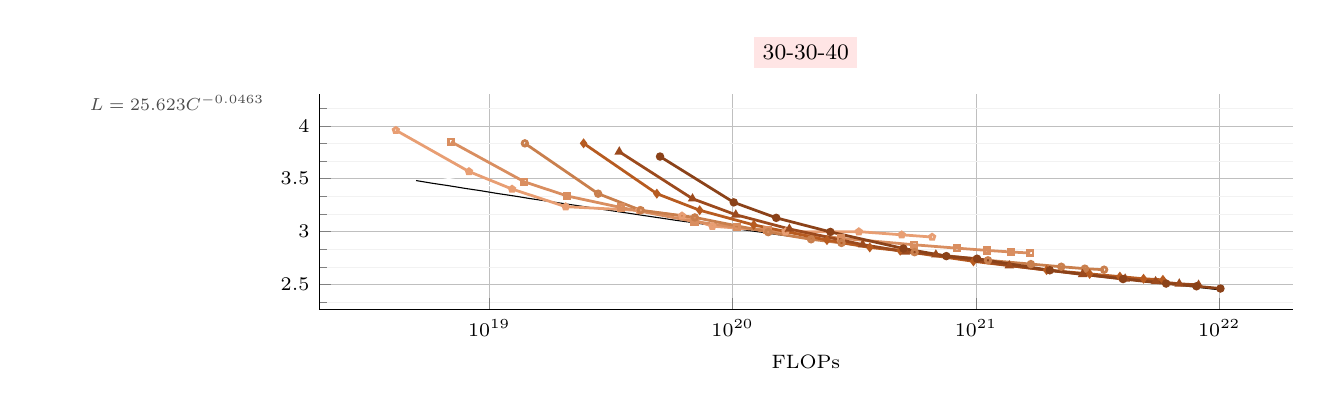
\begin{tikzpicture}
    \begin{axis}[
        legend pos=north east,
        grid=both,
        grid style={line width=.1pt, draw=gray!10},
        major grid style={line width=.2pt,draw=gray!50},
        minor tick num=2,
        axis x line*=bottom,
        axis y line*=left,
        xmode=log,
        log basis x=10,
        xtick={
            1E+19,
            1E+20,
            1E+21,
            1E+22
        },
        xmin=2E+18,
        xmax=2E+22,
        ymax=4.3,
        height=1.7in,
        width=1.15\linewidth,
        ylabel style={align=center, font=\scriptsize, yshift=-1ex},
        xlabel style={font=\scriptsize},
        title=\footnotesize{\colorbox{red!10}{30-30-40}},
        xlabel={\scriptsize{FLOPs}},
        yticklabel style={font=\scriptsize},
        xticklabel style={font=\scriptsize},
        legend style={cells={align=left}, font=\scriptsize, fill opacity=0.7, fill=none,  draw=none,at={(-0.3,0.95)}, anchor=west},
        legend cell align={left},
        mark options={solid},
    ]

    \addplot[color=white, samples=50, domain=5e18:10e21, mark=none] {29.574*x^(-0.04919)};
    \addlegendentry{\scalebox{0.9}{$L = 25.623C^{-0.0463}$}};
    \addplot[color=black, samples=50, domain=5e18:10e21] {25.622649599876997*x^(-0.04634327762259929)};

    \addplot[legend early_0_2b style, mark size=1pt] plot coordinates {
        (4.13e+18, 3.9586666666666672)
        (8.25e+18, 3.568)
        (1.24e+19, 3.402333333333333)
        (2.06e+19, 3.235666666666667)
        (4.13e+19, 3.200333333333333)
        (6.19e+19, 3.1493333333333333)
        (8.25e+19, 3.0506666666666664)
        (1.65e+20, 2.9996666666666663)
        (3.3e+20, 2.9996666666666663)
        (4.95e+20, 2.969666666666667)
        (6.6e+20, 2.9486666666666665)
    };
    \addplot[legend early_0_4b style, mark size=1pt] plot coordinates {
        (6.96e+18, 3.8503333333333334)
        (1.39e+19, 3.472)
        (2.09e+19, 3.3366666666666664)
        (3.48e+19, 3.2273333333333336)
        (6.96e+19, 3.095)
        (1.04e+20, 3.0406666666666666)
        (1.39e+20, 3.016)
        (2.78e+20, 2.9373333333333336)
        (5.57e+20, 2.8753333333333337)
        (8.35e+20, 2.8433333333333333)
        (1.11e+21, 2.8223333333333334)
        (1.39e+21, 2.8073333333333337)
        (1.67e+21, 2.797333333333333)
    };
    \addplot[legend early_0_9b style, mark size=1pt] plot coordinates {
        (1.4e+19, 3.8346666666666667)
        (2.8e+19, 3.3586666666666662)
        (4.19e+19, 3.202)
        (6.99e+19, 3.1340000000000003)
        (1.4e+20, 2.9949999999999997)
        (2.1e+20, 2.9273333333333333)
        (2.8e+20, 2.8930000000000002)
        (5.59e+20, 2.8053333333333335)
        (1.12e+21, 2.728333333333333)
        (1.68e+21, 2.692666666666667)
        (2.24e+21, 2.667666666666667)
        (2.8e+21, 2.6496666666666666)
        (3.36e+21, 2.639666666666667)
    };

    \addplot[legend early style, mark size=1pt] plot coordinates {
        (2.44e+19, 3.8346666666666667)
        (4.88e+19, 3.3586666666666662)
        (7.32e+19, 3.202)
        (1.22e+20, 3.063333333333334)
        (2.44e+20, 2.9196666666666666)
        (3.66e+20, 2.8503333333333334)
        (4.88e+20, 2.8196666666666665)
        (9.76e+20, 2.719)
        (1.95e+21, 2.6359999999999997)
        (2.93e+21, 2.6)
        (3.9e+21, 2.574)
        (4.88e+21, 2.554)
        (5.86e+21, 2.5436666666666667)
    };

    \addplot[legend early_2_2b style, mark size=1pt] plot coordinates {
        (3.42e+19, 3.755333333333333)
        (6.84e+19, 3.311)
        (1.03e+20, 3.159333333333333)
        (1.71e+20, 3.025)
        (3.42e+20, 2.8770000000000002)
        (5.13e+20, 2.8089999999999997)
        (6.84e+20, 2.781333333333333)
        (1.37e+21, 2.679)
        (2.74e+21, 2.595)
        (4.1e+21, 2.5536666666666665)
        (5.47e+21, 2.5283333333333333)
        (6.84e+21, 2.5066666666666664)
        (8.21e+21, 2.4953333333333334)
    };
    \addplot[legend early_3_3b style, mark size=1pt] plot coordinates {
        (5.03e+19, 3.7100000000000004)
        (1.01e+20, 3.276666666666667)
        (1.51e+20, 3.1300000000000003)
        (2.52e+20, 2.997)
        (5.03e+20, 2.84)
        (7.55e+20, 2.768333333333333)
        (1.01e+21, 2.7436666666666665)
        (2.01e+21, 2.6343333333333336)
        (4.02e+21, 2.5513333333333335)
        (6.04e+21, 2.5086666666666666)
        (8.05e+21, 2.483)
        (1.01e+22, 2.4616666666666664)
    };

\end{axis}
\end{tikzpicture}

    \end{subfigure}
    \begin{subfigure}[t]{0.24\linewidth}
        
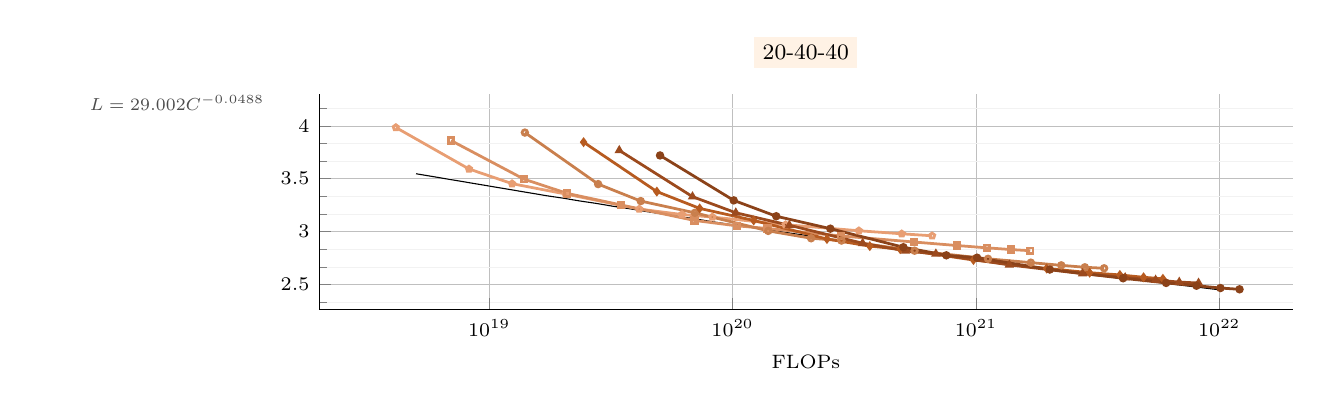
\begin{tikzpicture}
    \begin{axis}[
        legend pos=north east,
        grid=both,
        grid style={line width=.1pt, draw=gray!10},
        major grid style={line width=.2pt,draw=gray!50},
        minor tick num=2,
        axis x line*=bottom,
        axis y line*=left,
        xmode=log, %
        log basis x=10, %
        xtick={
            1E+19,
            1E+20,
            1E+21,
            1E+22
        },
        xmin=2E+18,
        xmax=2E+22,
        ymax=4.3,
        height=1.7in,
        width=1.15\linewidth,
        ylabel style={align=center, font=\scriptsize, yshift=-1ex},
        xlabel style={font=\scriptsize},
        title={\footnotesize{\colorbox{orange!10}{20-40-40}}},
        xlabel={\scriptsize{FLOPs}},
        yticklabel style={font=\scriptsize},
        xticklabel style={font=\scriptsize},
        legend style={cells={align=left}, font=\scriptsize, fill opacity=0.7, fill=none,  draw=none,at={(-0.3,0.95)}, anchor=west}, %
        legend cell align={left},
        mark options={solid},
    ]

    \addplot[color=white, samples=50, domain=5e18:10e21, mark=none] {29.574*x^(-0.04919)};
    \addlegendentry{\scalebox{0.9}{$L = 29.002C^{-0.0488}$}};
    \addplot[color=black, samples=50, domain=5e18:10e21] {29.002272950965768*x^(-0.04878835579770303)};

    \addplot[legend early_0_2b style, mark size=1pt] plot coordinates {
        (4.13e+18, 3.984666666666667)
        (8.25e+18, 3.592333333333334)
        (1.24e+19, 3.453333333333333)
        (2.06e+19, 3.3553333333333337)
        (4.13e+19, 3.2129999999999996)
        (6.19e+19, 3.1616666666666666)
        (8.25e+19, 3.1376666666666666)
        (1.65e+20, 3.0653333333333332)
        (3.3e+20, 3.0080000000000005)
        (4.95e+20, 2.9793333333333334)
        (6.6e+20, 2.9603333333333333)
    };
    \addplot[legend early_0_4b style, mark size=1pt] plot coordinates {
        (6.96e+18, 3.861333333333333)
        (1.39e+19, 3.4956666666666667)
        (2.09e+19, 3.361333333333333)
        (3.48e+19, 3.2516666666666665)
        (6.96e+19, 3.1056666666666666)
        (1.04e+20, 3.0546666666666664)
        (1.39e+20, 3.0293333333333337)
        (2.78e+20, 2.959)
        (5.57e+20, 2.9013333333333335)
        (8.35e+20, 2.8683333333333336)
        (1.11e+21, 2.8463333333333334)
        (1.39e+21, 2.8303333333333334)
        (1.67e+21, 2.8193333333333332)
    };
    \addplot[legend early_0_9b style, mark size=1pt] plot coordinates {
        (1.4e+19, 3.936666666666667)
        (2.8e+19, 3.449333333333333)
        (4.19e+19, 3.2886666666666664)
        (6.99e+19, 3.177666666666667)
        (1.4e+20, 3.0066666666666664)
        (2.1e+20, 2.937)
        (2.8e+20, 2.9153333333333333)
        (5.59e+20, 2.8193333333333332)
        (1.12e+21, 2.7426666666666666)
        (1.68e+21, 2.7063333333333333)
        (2.24e+21, 2.6809999999999996)
        (2.8e+21, 2.6626666666666665)
        (3.36e+21, 2.6533333333333338)
    };

    \addplot[legend early style, mark size=1pt] plot coordinates {
        (2.44e+19, 3.8456666666666663)
        (4.88e+19, 3.3783333333333334)
        (7.32e+19, 3.2193333333333336)
        (1.22e+20, 3.1056666666666666)
        (2.44e+20, 2.9299999999999997)
        (3.66e+20, 2.8626666666666662)
        (4.88e+20, 2.834)
        (9.76e+20, 2.731333333333333)
        (1.95e+21, 2.651333333333333)
        (2.93e+21, 2.611333333333333)
        (3.9e+21, 2.590333333333333)
        (4.88e+21, 2.568)
        (5.86e+21, 2.553666666666667)
    };

    \addplot[legend early_2_2b style, mark size=1pt] plot coordinates {
        (3.42e+19, 3.7680000000000002)
        (6.84e+19, 3.3303333333333334)
        (1.03e+20, 3.1780000000000004)
        (1.71e+20, 3.06)
        (3.42e+20, 2.89)
        (5.13e+20, 2.817)
        (6.84e+20, 2.7896666666666667)
        (1.37e+21, 2.685)
        (2.74e+21, 2.6020000000000003)
        (4.1e+21, 2.5646666666666667)
        (5.47e+21, 2.5420000000000003)
        (6.84e+21, 2.5226666666666664)
        (8.21e+21, 2.513666666666667)
    };
    \addplot[legend early_3_3b style, mark size=1pt] plot coordinates {
        (5.03e+19, 3.720333333333334)
        (1.01e+20, 3.2953333333333332)
        (1.51e+20, 3.1453333333333333)
        (2.52e+20, 3.0276666666666667)
        (5.03e+20, 2.8523333333333336)
        (7.55e+20, 2.7756666666666674)
        (1.01e+21, 2.753)
        (2.01e+21, 2.6413333333333333)
        (4.02e+21, 2.558666666666667)
        (6.04e+21, 2.514666666666667)
        (8.05e+21, 2.4883333333333337)
        (1.01e+22, 2.466333333333333)
        (1.21e+22, 2.454333333333333)
    };


    \end{axis}
\end{tikzpicture}
    \end{subfigure}
    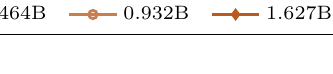
\begin{tikzpicture}
        \node[anchor=north] (legend) at (0\linewidth, 0) {
            \begin{axis}[
                        hide axis,
                        xmin=0, xmax=0.5, ymin=0, ymax=1,
                        legend columns=6,
                        legend style={
                            at={(-0.12, 0.05)},
                            anchor=north,
                            /tikz/every even column/.append style={column sep=0.2cm},
                            scale=0.5,
                            cells={align=left}, font=\scriptsize,
                            anchor=center,
                        },
                    ]
                \addlegendimage{legend early_0_2b style}
                \addlegendentry{0.275B}
                \addlegendimage{legend early_0_4b style}
                \addlegendentry{0.464B}
                \addlegendimage{legend early_0_9b style}
                \addlegendentry{0.932B}
                \addlegendimage{legend early style}
                \addlegendentry{1.627B}
                \addlegendimage{legend early_2_2b style}
                \addlegendentry{2.280B}
                \addlegendimage{legend early_3_3b style}
                \addlegendentry{3.354B}
            \end{axis}
        };
    \end{tikzpicture}
    \caption{\textbf{不同训练混合的尺度定律。}
    在改变预训练混合时,早期融合模型遵循类似的尺度变化趋势。然而,增加图像描述会导致更高的尺度指数范数(见~\cref{tab:scaling_laws_coeffs_data_mixtures})。
    }
    \label{fig:early_scaleflops_data_mixtures}
\end{figure*}


We conduct a similar study on late-fusion models
in~\cref{fig:early_vs_late_scaleflops_3d}~(right) and observe comparable scaling
behaviors. In particular, the loss scaling exponent ($c = -0.0494$) is nearly
identical to that of early fusion ($c = -0.0492$).  
This trend is evident in \cref{fig:early_vs_late_scaleflops}, where early fusion
outperforms late fusion at smaller model scales, while both architectures
converge to similar performance at larger model sizes. We also observe similar
trends when varying late-fusion configurations, such as using a smaller vision
encoder with a larger text decoder~\cref{app:late_vs_early}.


\begin{figure}[t!]
    \begin{minipage}[t]{0.48\textwidth}
            \centering
    \captionsetup{type=figure}
    \begin{subfigure}[t]{0.49\linewidth}
        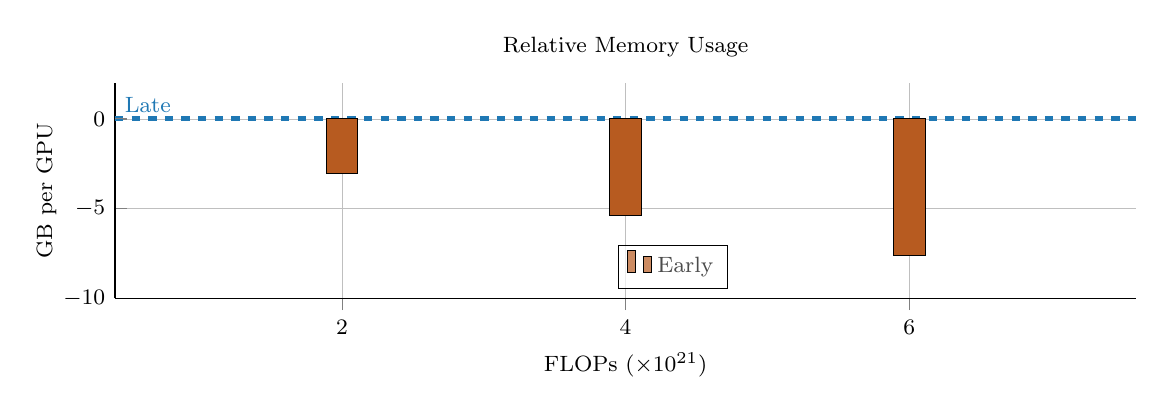
\begin{tikzpicture}
    \begin{axis}[
        ybar,
        bar width=20pt,
        enlarge x limits=0.4,
        legend pos=north east,
        grid=both,
        grid style={line width=.1pt, draw=gray!10},
        major grid style={line width=.2pt,draw=gray!50},
        axis x line*=bottom,
        axis y line*=left,
        xtick={
            2,
            4,
            6
        },
        height=1.7in,
        width=1.2\linewidth,
        ylabel style={align=center, font=\footnotesize, yshift=-1ex},
        xlabel style={font=\footnotesize},
        title={\footnotesize{Relative Memory Usage}},
        ylabel={\footnotesize{GB per GPU}},
        xlabel={\footnotesize{FLOPs ($\times10^{21}$)}},
        yticklabel style={font=\footnotesize},
        xticklabel style={font=\footnotesize},
        legend style={cells={align=left}, font=\footnotesize, fill opacity=0.7, at={(0.6,0.25)}},
        legend cell align={left},
        ymin=-10,
        ymax=2,
        extra y ticks={0.03},
        extra y tick labels={},
        extra y tick style={grid=major, major grid style={line width=2pt, draw=LateColor, dashed}},
    ]
        \addplot[legend early bars style] coordinates {
            (2,-3.05)
            (4,-5.38)
            (6,-7.59)
        };
        \addlegendentry{Early}
        \node[anchor=west, font=\footnotesize, text=LateColor] at (axis cs:0.4,0.8) {Late};
    \end{axis}
    \end{tikzpicture}

    \end{subfigure}
    \begin{subfigure}[t]{0.49\linewidth}
        
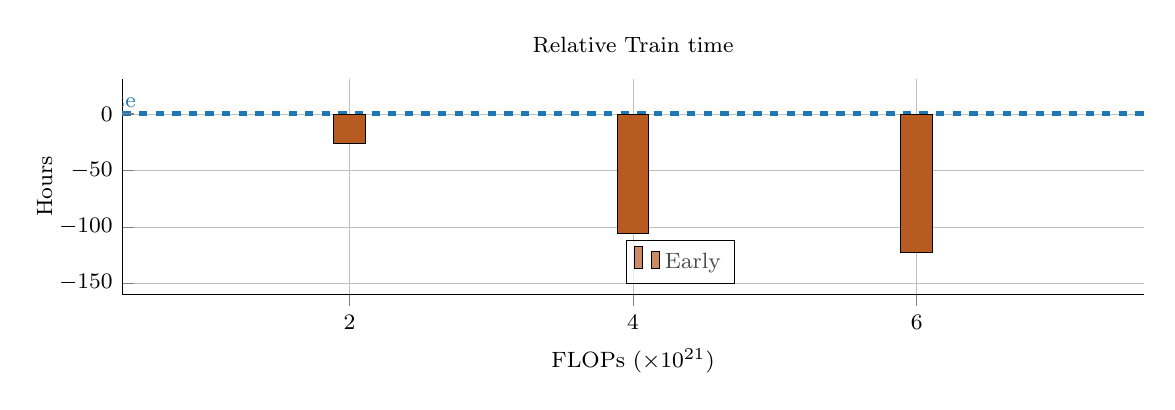
\begin{tikzpicture}
    \begin{axis}[
        ybar, %
        bar width=16pt, %
        enlarge x limits=0.4, %
        legend pos=north east,
        grid=both,
        grid style={line width=.1pt, draw=gray!10},
        major grid style={line width=.2pt,draw=gray!50},
        axis x line*=bottom,
        axis y line*=left,
        xtick={
            2,
            4,
            6
        },
        height=1.7in,
        width=1.2\linewidth,
        ylabel style={align=center, font=\footnotesize, yshift=-1ex},
        xlabel style={font=\footnotesize},
        title={\footnotesize{Relative Train time}},
        ylabel={\footnotesize{Hours}},
        xlabel={\footnotesize{FLOPs ($\times10^{21}$)}},
        yticklabel style={font=\footnotesize},
        xticklabel style={font=\footnotesize},
        legend style={cells={align=left}, font=\footnotesize, fill opacity=0.7, at={(0.6, 0.25)}},
        legend cell align={left},
        ymin=-160,               %
        ymax=32,
        extra y ticks={1},
        extra y tick labels={},
        extra y tick style={grid=major, major grid style={line width=2pt, draw=LateColor, dashed}},
    ]

    \addplot[legend early bars style] coordinates {
        (2, -26)
        (4, -106)
        (6, -123)
    };
    \addlegendentry{Early}

    \node[anchor=west, font=\footnotesize, text=LateColor] at (axis cs:0.1,13) {Late};

    \end{axis}
\end{tikzpicture}

    \end{subfigure}
    \vspace{-3pt}
    \caption{\textbf{Early vs late: pretraining efficiency.} Early-fusion is faster to train and consumes less memory. Models are trained on 16 H100 GPUs for 160k steps (300B tokens).}
    \label{fig:early_vs_late_efficiency}

    \end{minipage}        
    \hfill
    \begin{minipage}[t]{0.48\textwidth}
        \centering
    \captionsetup{type=figure}
    \begin{subfigure}[t]{0.49\linewidth}
        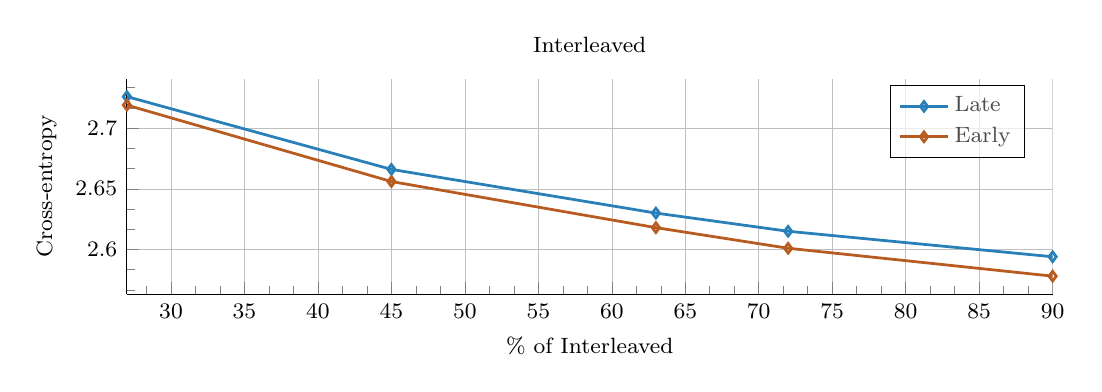
\begin{tikzpicture}
    \begin{axis}[
        legend pos=north east,
        grid=major,
        grid style={line width=.1pt, draw=gray!30},
        major grid style={line width=.2pt,draw=gray!50},
        minor tick num=2,
        axis x line*=bottom,
        axis y line*=left,
        xmin=27,
        xmax=90,
        height=1.7in,
        width=1.1\linewidth,
        ylabel style={align=center, font=\footnotesize},
        xlabel style={font=\footnotesize},
        ylabel=\footnotesize{Cross-entropy},
        xlabel={\footnotesize{\% of Interleaved}},
        title=\footnotesize{Interleaved},
        ytick distance=0.05,
        yticklabel style={font=\footnotesize, /pgf/number format/fixed, /pgf/number format/precision=2},
        xticklabel style={font=\footnotesize},
        mark options={solid},
        legend style={cells={align=left}, font=\footnotesize, fill opacity=0.7},
        legend cell align={left},
    ]

\addplot[legend late style, mark size=1.75pt] plot coordinates {
    (27, 2.726)
    (45, 2.666)
    (63, 2.63)
    (72, 2.615)
    (90, 2.594)
};
\addlegendentry{Late}

\addplot[legend early style, mark size=1.75pt] plot coordinates {
    (27, 2.719)
    (45, 2.656)
    (63, 2.618)
    (72, 2.601)
    (90, 2.578)
};
\addlegendentry{Early}

\end{axis}
\end{tikzpicture}

    \end{subfigure}
    \begin{subfigure}[t]{0.49\linewidth}
        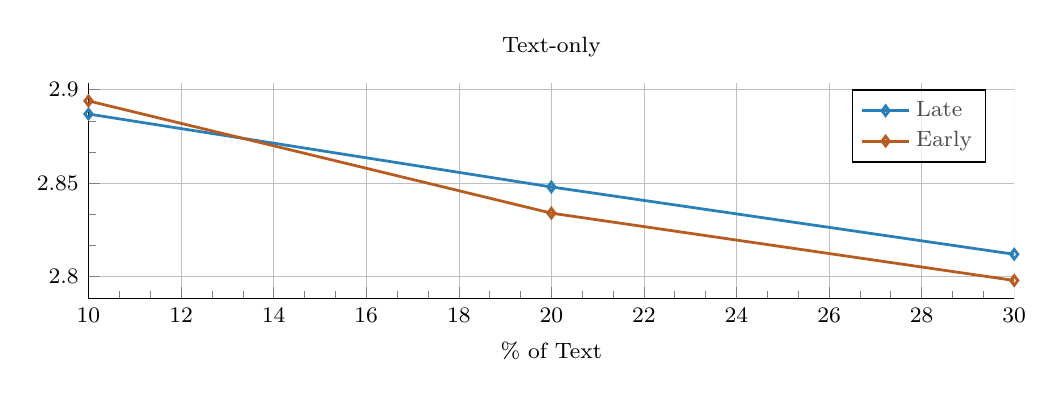
\begin{tikzpicture}
    \begin{axis}[
        legend pos=north east,
        grid=major,
        grid style={line width=.1pt, draw=gray!30},
        major grid style={line width=.2pt,draw=gray!50},
        minor tick num=2,
        axis x line*=bottom,
        axis y line*=left,
        xmin=10,
        xmax=30,
        height=1.7in,
        width=1.1\linewidth,
        ylabel style={align=center, font=\footnotesize, yshift=-1ex},
        xlabel style={font=\footnotesize},
        title=\footnotesize{Text-only},
        ytick distance=0.05,
        yticklabel style={font=\footnotesize, /pgf/number format/fixed, /pgf/number format/precision=2},
        xlabel={\footnotesize{\% of Text}},
        xticklabel style={font=\footnotesize},
        legend style={cells={align=left}, font=\footnotesize, fill opacity=0.7},
        legend cell align={left},
    ]

    \addplot[legend late style, mark size=1.75pt] plot coordinates {
    (10, 2.887)
    (20, 2.848)
    (30, 2.812)
    };
    \addlegendentry{Late}

    \addplot[legend early style, mark size=1.75pt] plot coordinates {
    (10, 2.894)
    (20, 2.834)
    (30, 2.798)
    };
    \addlegendentry{Early}

\end{axis}
\end{tikzpicture}

    \end{subfigure}
    \caption{\textbf{早期融合 vs 晚期融合:改变训练混合方式。}我们对训练混合方式进行调整,并绘制最终的训练损失。当增加交错文档与纯文本数据的比例时,早期融合模型表现更优。}
    \label{fig:early_vs_late_datatype_interleaved_text_main}

    \end{minipage}
\end{figure}



\cpar{Scaling laws of NMMs \textit{vs} LLMs.}
Upon comparing the scaling law coefficients of our NMMs to those reported for
text-only LLMs (\eg, GPT-3, Chinchilla), we find them to be within similar
ranges. In particular, for predicting the loss as a function of compute,
GPT-3~\citep{brown2020language} follows $L \propto C^{-0.048}$, while our models
follow $L \propto C^{-0.049}$, suggesting that the performance of NMMs adheres
to similar scaling laws as LLMs.  
Similarly, our estimates of the $\alpha$ and $\beta$ parameters in
\cref{eq:scaling_laws} ($\alpha=0.301$, $\beta=0.335$) closely match those
reported by~\citet{hoffmann2022training} ($\alpha=0.339$, $\beta=0.285$).
Likewise, our computed values of $a=0.526$ and $b=0.473$ align closely with
$a=0.46$ and $b=0.54$ from~\citet{hoffmann2022training}, reinforcing the idea
that, for native multimodal models, the number of training tokens and model
parameters should be scaled proportionally.  
However, since the gap between $a$ and $b$ is smaller than in LLMs, this
principle holds even more strongly for NMMs. Additionally, as $a=0.526$ is
greater than $b=0.473$ in our case, the optimal model size for NMMs is larger
than that of LLMs, while the optimal number of training tokens is lower, given
a fixed compute budget. 



\cpar{Compute-optimal trade-offs for early \textit{vs.} late fusion NMMs.}  
While late- and early-fusion models reduce loss at similar rates with increasing
FLOPs, we observe distinct trade-offs in their compute-optimal models.
Specifically, $N_{opt}$ is larger for late-fusion models, whereas $D_{opt}$ is
larger for early-fusion models. This indicates that, given a fixed compute
budget, late-fusion models require a higher number of parameters, while early-fusion
models benefit more from a higher number of training tokens.  
This trend is also reflected in the lower $\frac{N_{opt}}{D_{opt}} \propto
C^{0.053}$ for early fusion compared to $\frac{N_{opt}}{D_{opt}} \propto
C^{0.076}$ for late fusion. As shown in \cref{fig:teaser}~(right), when scaling FLOPs,
the number of parameters of early fusion models becomes significantly lower, which is crucial
for reducing inference costs and, consequently, lowering serving costs after
deployment.  


\begin{table}[t!]
    \centering
    \setlength{\tabcolsep}{12pt}
    \renewcommand{\arraystretch}{1}
    \resizebox{\linewidth}{!}{
    \begin{tabular}{lcccccccccc}
        & C-I-T (\%) & I/T ratio &  E & $\alpha$ & $\beta$ & a & b  & d & c \\ %
        \shline
        1 & \colorbox{blue!10}{45-45-10}  & 1.19 & 1.906  & 0.301  & 0.335  & 0.527  & 0.474   & 0.901  & -0.0492 \\%& 58.35\\
        2 & \colorbox{red!10}{40-20-40}  & 0.65 &  1.965  & 0.328  & 0.348  & 0.518  & 0.486   & 0.937  & -0.0486 \\
        3 & \colorbox{green!10}{30-30-40}  & 0.59 & 1.847  & 0.253  & 0.338  & 0.572  & 0.428   & 0.748  & -0.0463 \\
        4 & \colorbox{orange!10}{20-40-40}  & 0.49 &  1.836  & 0.259  & 0.354  & 0.582  & 0.423   & 0.726  & -0.0488 \\
    \end{tabular}%
    } \caption{\textbf{Scaling laws for different training mixtures}. Early-fusion models. C-I-T refer to image-caption, interleaved and text}
    \label{tab:scaling_laws_coeffs_data_mixtures}
\end{table}


\cpar{Early-fusion is more efficient to train.}
We compare the training efficiency of late- and early-fusion architectures. As shown in \cref{fig:early_vs_late_efficiency}, early-fusion models consume less memory and train faster under the same compute budget. This advantage becomes even more pronounced as compute increases, highlighting the superior training efficiency of early fusion while maintaining comparable performance to late fusion at scale. Notably, for the same FLOPs, late-fusion models have a higher parameter count and higher effective depth (\ie, additional vision encoder layers alongside decoder layers) compared to early-fusion models.




\begin{figure*}[h!]
    \centering
    \captionsetup{type=figure}
    
    \begin{minipage}[t]{0.55\linewidth}
        \centering
        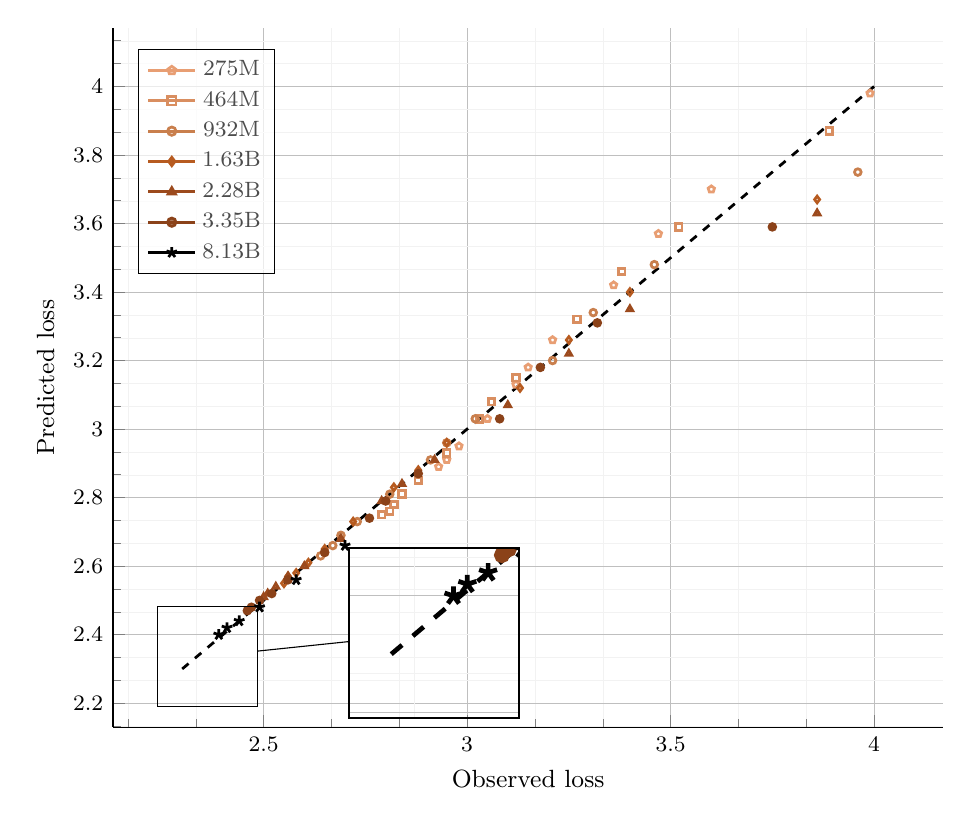
\begin{tikzpicture}[
    spy using outlines={rectangle, magnification=1.7, size=0.85in, connect spies}
]
    \begin{axis}[
        legend pos=north west,
        grid=both,
        grid style={line width=.1pt, draw=gray!10},
        major grid style={line width=.2pt, draw=gray!50},
        minor tick num=2,
        axis x line*=bottom,
        axis y line*=left,
        width=1\linewidth,
        xtick distance=0.5,
        ylabel={\small{Predicted loss}},
        xlabel={\small{Observed loss}},
        yticklabel style={font=\footnotesize},
        xticklabel style={font=\footnotesize},
        legend style={cells={align=left}, font=\footnotesize, fill opacity=0.7},
        mark options={solid},
    ]

    \addlegendimage{legend early_0_2b style}
    \addlegendentry{275M}
    \addlegendimage{legend early_0_4b style}
    \addlegendentry{464M}
    \addlegendimage{legend early_0_9b style}
    \addlegendentry{932M}
    \addlegendimage{legend early style}
    \addlegendentry{1.63B}
    \addlegendimage{legend early_2_2b style}
    \addlegendentry{2.28B}
    \addlegendimage{legend early_3_3b style}
    \addlegendentry{3.35B}
    \addlegendimage{legend early_8b style}
    \addlegendentry{8.13B}

    \addplot[line width=1pt, dashed, color=black, samples=50, domain=2.3:4.0] {x};

    \addplot[legend early_0_2b style,, only marks, mark size=1.2pt] plot coordinates {
        (3.99E+00, 3.98E+00)
        (3.60E+00, 3.70E+00)
        (3.47E+00, 3.57E+00)
        (3.36E+00, 3.42E+00)
        (3.21E+00, 3.26E+00)
        (3.15E+00, 3.18E+00)
        (3.12E+00, 3.13E+00)
        (3.05E+00, 3.03E+00)
        (2.98E+00, 2.95E+00)
        (2.95E+00, 2.91E+00)
        (2.93E+00, 2.89E+00)
    };
    \addplot[legend early_0_4b style, only marks, mark size=1.2pt] plot coordinates {
        (3.89E+00, 3.87E+00)
        (3.52E+00, 3.59E+00)
        (3.38E+00, 3.46E+00)
        (3.27E+00, 3.32E+00)
        (3.12E+00, 3.15E+00)
        (3.06E+00, 3.08E+00)
        (3.03E+00, 3.03E+00)
        (2.95E+00, 2.93E+00)
        (2.88E+00, 2.85E+00)
        (2.84E+00, 2.81E+00)
        (2.82E+00, 2.78E+00)
        (2.81E+00, 2.76E+00)
        (2.79E+00, 2.75E+00)
    };
    \addplot[legend early_0_9b style, only marks, mark size=1.2pt] plot coordinates {
        (3.96E+00, 3.75E+00)
        (3.46E+00, 3.48E+00)
        (3.31E+00, 3.34E+00)
        (3.21E+00, 3.20E+00)
        (3.02E+00, 3.03E+00)
        (2.95E+00, 2.96E+00)
        (2.91E+00, 2.91E+00)
        (2.81E+00, 2.81E+00)
        (2.73E+00, 2.73E+00)
        (2.69E+00, 2.69E+00)
        (2.67E+00, 2.66E+00)
        (2.65E+00, 2.64E+00)
        (2.64E+00, 2.63E+00)
    };

    \addplot[legend early style, only marks, mark size=1.2pt] plot coordinates {
        (3.86E+00, 3.67E+00)
        (3.40E+00, 3.40E+00)
        (3.25E+00, 3.26E+00)
        (3.13E+00, 3.12E+00)
        (2.95E+00, 2.96E+00)
        (2.88E+00, 2.88E+00)
        (2.82E+00, 2.83E+00)
        (2.72E+00, 2.73E+00)
        (2.65E+00, 2.65E+00)
        (2.61E+00, 2.61E+00)
        (2.58E+00, 2.58E+00)
        (2.56E+00, 2.57E+00)
        (2.55E+00, 2.55E+00)
    };

    \addplot[legend early_2_2b style, only marks, mark size=1.2pt] plot coordinates {
        (3.86E+00, 3.63E+00)
        (3.40E+00, 3.35E+00)
        (3.25E+00, 3.22E+00)
        (3.10E+00, 3.07E+00)
        (2.92E+00, 2.91E+00)
        (2.84E+00, 2.84E+00)
        (2.79E+00, 2.79E+00)
        (2.69E+00, 2.68E+00)
        (2.60E+00, 2.60E+00)
        (2.56E+00, 2.57E+00)
        (2.53E+00, 2.54E+00)
        (2.51E+00, 2.52E+00)
        (2.50E+00, 2.51E+00)
    };
    \addplot[legend early_3_3b style, only marks, mark size=1.2pt] plot coordinates {
        (3.75E+00, 3.59E+00)
        (3.32E+00, 3.31E+00)
        (3.18E+00, 3.18E+00)
        (3.08E+00, 3.03E+00)
        (2.88E+00, 2.87E+00)
        (2.80E+00, 2.79E+00)
        (2.76E+00, 2.74E+00)
        (2.65E+00, 2.64E+00)
        (2.56E+00, 2.56E+00)
        (2.52E+00, 2.52E+00)
        (2.49E+00, 2.50E+00)
        (2.47E+00, 2.48E+00)
        (2.46E+00, 2.47E+00)
    };

    \addplot[legend early_8b style, only marks, mark size=2pt] plot coordinates {
        (2.70E+00, 2.66E+00)
        (2.58E+00, 2.56E+00)
        (2.49E+00, 2.48E+00)
        (2.44E+00, 2.44E+00)
        (2.41E+00, 2.42E+00)
        (2.39E+00, 2.40E+00)
    };

    \begin{scope}
        \spy on (1.2,0.9) in node [right] at (3,1.2);
    \end{scope}

\end{axis}
\end{tikzpicture}

        \caption{\textbf{Observed vs predicted loss.} We visualize the loss predicted by our scaling laws \cref{eq:scaling_laws} and the actual loss achieved by each run. We can reliably predict the performance of models larger (8B params) than those used to fit the scaling laws.}
        \label{fig:observed_vs_predicted_loss_extrapolation}
    \end{minipage}
    \hfill
    \begin{minipage}[t]{0.4\linewidth}
        \begin{minipage}[t]{\linewidth}
            \centering
            \vspace{-5.5cm}
            \setlength{\tabcolsep}{8pt} %
            \renewcommand{\arraystretch}{1} %
            \resizebox{1.0\linewidth}{!}{
            \begin{tabular}{lccc}
                Parameter & MSE & R2 & MAE (\%) \\
                \shline
                Held-in      & 0.0029  & 0.9807 & 0.8608 \\
                Held-out     & 0.0004 & 0.9682 & 0.5530 \\
            \end{tabular}%
            }
            \captionof{table}{\textbf{Scaling laws prediction errors.} We report the mean square error, R2 and mean absolute error for the loss prediction for held-in and held-out (8B model) data.}
            \label{tab:scaling_laws_errors_main}
        \end{minipage}
        
        \begin{minipage}[t]{\linewidth}
            \centering
            \vspace{-2.8cm}
            \setlength{\tabcolsep}{12pt} %
            \renewcommand{\arraystretch}{1} %
            \resizebox{\linewidth}{!}{
            \begin{tabular}{lcc}
                Parameter & Avg & Std \\
                \shline
                $E$      & 1.80922  & 0.33811  \\
                $\alpha$ & 0.29842  & 0.10101  \\
                $\beta$  & 0.33209  & 0.02892  \\
                $a$      & 0.54302  & 0.08813  \\
                $b$      & 0.48301  & 0.05787  \\
                $d$      & 0.92375  & 0.23296  \\
            \end{tabular}%
            }
            \captionof{table}{\textbf{Scaling laws sensitivity.} We report the mean and standard deviation after bootstrapping with 100 iterations.}
            \label{tab:scaling_laws_sensitivity_main}
        \end{minipage}
    \end{minipage}
\end{figure*}


    

\subsection{\edit{Scaling laws evaluation}}
\label{sec:scaling_laws_evaluation}
For each model size and number of training tokens, we compute the loss using the
estimated functional form in \cref{eq:scaling_laws} and compare it to the actual
loss observed in our runs. \Cref{fig:observed_vs_predicted_loss_extrapolation}
and \Cref{tab:scaling_laws_errors_main} visualizes these comparisons, showing
that our estimation is highly accurate, particularly for lower loss values and
larger FLOPs. We also assess our scaling laws in an extrapolation setting,
predicting performance beyond the model sizes used for fitting. Notably, our
approach estimates the performance of an 8B model with reasonable accuracy.  

Additionally, we conduct a sensitivity analysis using bootstrapping.
Specifically, we sample \( P \) points with replacement (\( P \) being the total
number of trained models) and re-estimate the scaling law coefficients. This
process is repeated 100 times, and we report the mean and standard deviation of
each coefficient. \Cref{tab:scaling_laws_sensitivity_main} shows that our
estimation is more precise for \(\beta\) than for \(\alpha\), primarily due to
the smaller number of model sizes relative to the number of different token
counts used to derive the scaling laws.





\subsection{Scaling laws for different data mixtures}
\label{sec:scaling_data_mix}
We investigate how variations in the training mixture affect the scaling laws of
native multimodal models. To this end, we study four different mixtures that
reflect common community
practices~\citep{laurenccon2024obelics,mckinzie2025mm1,zhang2024mm1_5,lin2024vila},
with Image Caption-Interleaved-Text ratios of \colorbox{blue!10}{45-45-10} (our default setup),
\colorbox{red!10}{30-30-40}, \colorbox{green!10}{40-20-40}, and \colorbox{orange!10}{20-40-40}.  
For each mixture, we conduct a separate scaling study by training 76 different
models, following our setup in \cref{sec:scaling_laws_early}. Overall,
\cref{fig:early_scaleflops_data_mixtures} shows that different mixtures follow
similar scaling trends; however, the scaling coefficients vary depending on the
mixture (\cref{tab:scaling_laws_coeffs_data_mixtures}). Interestingly,
increasing the proportion of image-caption data (mixtures 1 and 2) leads to
lower $a$ and higher $b$, whereas increasing the ratio of interleaved and text
data (mixtures 3 and 4) have the opposite effect.  
Notably, image-caption data contains more image tokens than text
tokens; therefore, increasing its proportion results in more
image tokens, while increasing interleaved and text data increases text token
counts. This suggests that, when image tokens are prevalent, training for longer decreases the loss faster than increasing the model size. 
We also found that for a fixed model size, increasing text-only and interleaved data ratio is in favor of
early-fusion \cref{fig:early_vs_late_datatype_interleaved_text_main}.


























\subsection{Native multimodal pre-training \textbf{\vs} continual training of
LLMs}
\label{sec:native_vs_continual}
In this section, we compare training natively from scratch to continual training
after initializing from a pre-trained LLM. We initialize the model from DCLM-1B~\citep{fang2023data} that is trained on more than 2T tokens.
\Cref{fig:early_vs_early_init_scaledata} shows that native multimodal models can
close the gap with initialized models when trained for longer.
Specifically, on image captioning data, the model requires fewer than 100B
multimodal tokens to reach comparable performance. However, on interleaved and
text data, the model may need longer training—up to 1T tokens.
Considering the cost of pre-training, these results suggest that training
natively could be a more efficient approach for achieving the same performance on multimodal benchmarks.

\begin{figure}[t!]
    \centering
    \captionsetup{type=figure}
    \begin{subfigure}[t]{0.32\linewidth}
        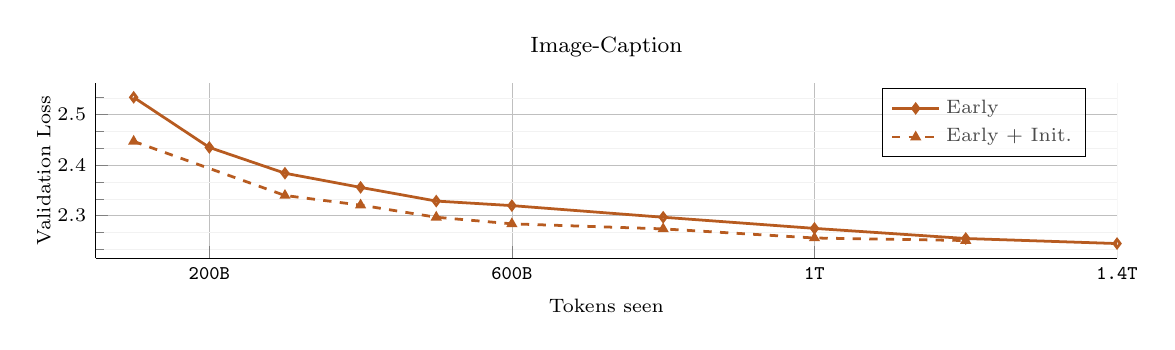
\begin{tikzpicture}
    \begin{axis}[
        legend pos=north east,
        grid=both,
        grid style={line width=.1pt, draw=gray!10},
        major grid style={line width=.2pt,draw=gray!50},
        minor tick num=2,
        axis x line*=bottom,
        axis y line*=left,
        xtick={
        0,
        0.2,
        0.6,
        1,
        1.4
        },
        xticklabels={
        \texttt{50B},
        \texttt{200B},
        \texttt{600B},
        \texttt{1T},
        \texttt{1.4T}
        },
        xmin=0.05,
        xmax=1.4,
        height=1.5in,
        width=1.2\linewidth,
        ylabel style={align=center, font=\scriptsize, yshift=-1ex},
        xlabel style={font=\scriptsize},
        title={\footnotesize{Image-Caption}},
        xlabel={\scriptsize{Tokens seen}},
        ylabel={\scriptsize{Validation Loss}},
        yticklabel style={font=\scriptsize},
        xticklabel style={font=\scriptsize},
        legend style={cells={align=left}, font=\scriptsize, fill opacity=0.7},
        legend cell align={left},
        mark options={solid},
    ]

\addplot[legend early style] plot coordinates {
        (0.1, 2.534)
        (0.2, 2.435)
        (0.3, 2.384)
        (0.4, 2.356)
        (0.5, 2.329)
        (0.6, 2.32)
        (0.8, 2.297)
        (1,   2.275)
        (1.2, 2.255)
        (1.4, 2.245)
    };
    \addlegendentry{\scalebox{1}{Early}}

\addplot[legend early_init style_dashed, mark=triangle*, mark size=1.35pt] plot coordinates {
        (0.1, 2.447)
        (0.3, 2.34)
        (0.4, 2.321)
        (0.5, 2.297)
        (0.6, 2.284)
        (0.8, 2.274)
        (1,   2.256)
        (1.2, 2.251)

    };
    \addlegendentry{\scalebox{1}{Early + Init.}}

\end{axis}
\end{tikzpicture}

    \end{subfigure}
    \hfill
    \begin{subfigure}[t]{0.31\linewidth}
        



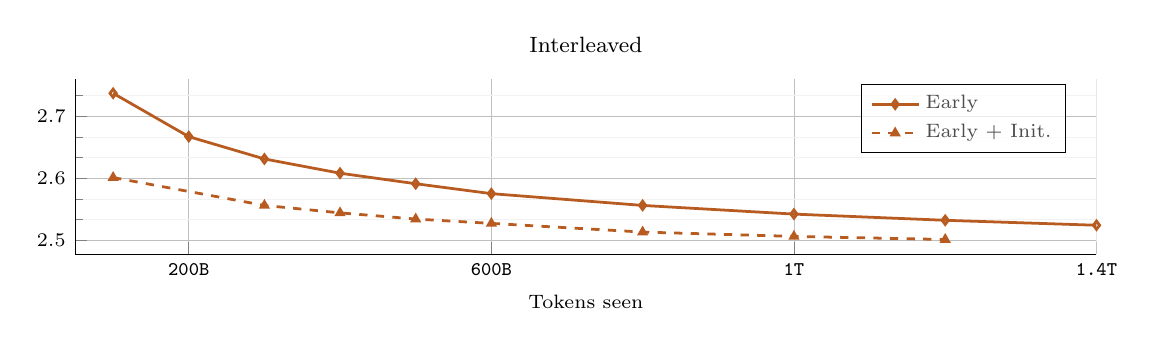
\begin{tikzpicture}
    \begin{axis}[
        legend pos=north east,
        grid=both,
        grid style={line width=.1pt, draw=gray!10},
        major grid style={line width=.2pt,draw=gray!50},
        minor tick num=2,
        axis x line*=bottom,
        axis y line*=left,
        xtick={
        0,
        0.2, 
        0.6,
        1,
        1.4
        },
        xticklabels={
        \texttt{50B}, 
        \texttt{200B}, 
        \texttt{600B},
        \texttt{1T},
        \texttt{1.4T}
        },
        xmin=0.05,
        xmax=1.4,
        height=1.5in,
        width=1.2\linewidth,
        ylabel style={align=center, font=\scriptsize, yshift=-1ex},
        xlabel style={font=\scriptsize},
        title={\footnotesize{Interleaved}},
        xlabel={\scriptsize{Tokens seen}},
        yticklabel style={font=\scriptsize},
        xticklabel style={font=\scriptsize},
        legend style={cells={align=left}, font=\scriptsize, fill opacity=0.7}, %
        legend cell align={left},
        mark options={solid},
    ]





    




    \addplot[legend early style] plot coordinates {
        (0.1, 2.737)
        (0.2, 2.667)
        (0.3, 2.631)
        (0.4, 2.608)
        (0.5, 2.591)       
        (0.6, 2.575) 
        (0.8, 2.556)
        (1,   2.542)
        (1.2, 2.532)
        (1.4, 2.524)
    };
    \addlegendentry{\scalebox{1}{Early}}





    \addplot[legend early_init style_dashed, mark=triangle*, mark size=1.35pt] plot coordinates {
        (0.1, 2.601)
        (0.3, 2.556)
        (0.4, 2.544)
        (0.5, 2.534)       
        (0.6, 2.527) 
        (0.8, 2.513)
        (1,   2.506)
        (1.2, 2.501)
    };
    \addlegendentry{\scalebox{1}{Early + Init.}}


    \end{axis}
\end{tikzpicture}
    \end{subfigure}
    \hfill
    \begin{subfigure}[t]{0.31\linewidth}
        
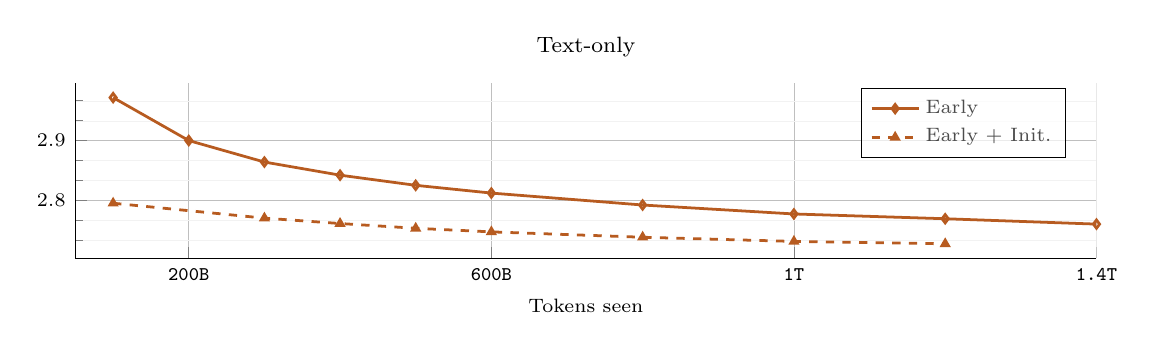
\begin{tikzpicture}
    \begin{axis}[
        legend pos=north east,
        grid=both,
        grid style={line width=.1pt, draw=gray!10},
        major grid style={line width=.2pt,draw=gray!50},
        minor tick num=2,
        axis x line*=bottom,
        axis y line*=left,
        xtick={
        0,
        0.2, 
        0.6,
        1,
        1.4
        },
        xticklabels={
        \texttt{50B}, 
        \texttt{200B}, 
        \texttt{600B},
        \texttt{1T},
        \texttt{1.4T}
        },
        xmin=0.05,
        xmax=1.4,
        height=1.5in,
        width=1.2\linewidth,
        ylabel style={align=center, font=\scriptsize, yshift=-1ex},
        xlabel style={font=\scriptsize},
        title={\footnotesize{Text-only}},
        xlabel={\scriptsize{Tokens seen}},
        yticklabel style={font=\scriptsize},
        xticklabel style={font=\scriptsize},
        legend style={cells={align=left}, font=\scriptsize, fill opacity=0.7}, %
        legend cell align={left},
        mark options={solid},
        legend style={cells={align=left}, font=\scriptsize, text=black}, %
    ]



    
    


    \addplot[legend early style] plot coordinates {
        (0.1, 2.972)
        (0.2, 2.9)
        (0.3, 2.864)
        (0.4, 2.842)
        (0.5, 2.825)
        (0.6, 2.812)
        (0.8, 2.792)
        (1,   2.777)
        (1.2, 2.769)
        (1.4, 2.76 )
    };
    \addlegendentry{\scalebox{1}{Early}}




    \addplot[legend early_init style_dashed, mark=triangle*, mark size=1.35pt] plot coordinates {
        (0.1, 2.795)
        (0.3, 2.77)
        (0.4, 2.761)
        (0.5, 2.753)
        (0.6, 2.747)
        (0.8, 2.738)
        (1, 2.731)
        (1.2, 2.727)
    };
    \addlegendentry{\scalebox{1}{Early + Init.}}



    \end{axis}
\end{tikzpicture}
    \end{subfigure}
    \vspace{-7pt}
    \caption{\textbf{早期原生与从LLMs初始化:从预训练模型初始化和扩展训练标记。} 我们比较了使用和不使用DCLM-1B初始化的训练。}
    \label{fig:early_vs_early_init_scaledata}
    \vspace{7pt}
\end{figure}





\section{\edit{Towards multimodal specialization}}
Previously, we demonstrated that early-fusion models achieve performance on par
with late-fusion models under a fixed compute budget. However, multimodal data
is inherently heterogeneous, and training a unified model to fit such diverse
distributions may be suboptimal.  
Here, we argue for multimodal specialization within a unified architecture.
Ideally, the model should implicitly adapt to each modality, for instance, by
learning modality-specific weights or specialized experts. MoEs is
a strong candidate for this approach, having demonstrated effectiveness in LLMs.  
In this section, we highlight the advantages of sparse early-fusion models over
their dense counterparts.



\cpar{Setup.} Our sparse models are based on the dropless-MoE implementation
of~\citet{gale2023megablocks}, which eliminates token dropping during training
caused by expert capacity constraints. We employ a top-$k$ expert-choice routing
mechanism, where each token selects its top-$k$ experts among the $E$ available
experts. Specifically, we set $k=1$ and $E=8$, as we find this configuration to
work effectively.  
Additionally, we incorporate an auxiliary load-balancing
loss~\citep{shazeer2017outrageously} with a weight of 0.01 to ensure a balanced
expert utilization. Following~\citet{abnar2025parameters}, we compute training
FLOPs as $6ND$, where $N$ represents the number of active parameters.  



\subsection{Sparse vs dense NMMs when scaling FLOPs}  
We compare sparse MoE models to their dense counterparts by training models with different numbers of active parameters and varying amounts of training tokens. \cref{fig:dense_vs_moe_scaledata} shows that, under the same inference cost (or number of active parameters), MoEs significantly outperform dense models.  
Interestingly, this performance gap is more pronounced for smaller model sizes. This suggests that MoEs enable models to handle heterogeneous data more effectively and specialize in different modalities. However, as dense models become sufficiently large, the gap between the two architectures gradually closes.


\vspace{15pt}
\subsection{Scaling laws for sparse early-fusion models}
We train different models (ranging from 300M to 3.4B active parameters) on
varying amounts of tokens (ranging from 250M to 600B) and report the final loss
in \cref{fig:early_scaleflops_moe_avg}. We fit a power law to the convex hull of
the lowest loss as a function of compute (FLOPs). Interestingly, the exponent
($-0.047$) is close to that of dense NMMs ($-0.049$), indicating that both
architectures scale similarly. However, the multiplicative constant is smaller
for MoEs ($26.287$) compared to dense models ($29.574$), revealing lower loss.
Additionally, MoEs require longer training to reach saturation compared to dense
models (\cref{app:scaling_laws} for more details). \edit{We also predict the
coefficients of \cref{eq:scaling_laws} by \edit{considering $N$ as the number of
active parameters. \Cref{tab:early_vs_late_coeffs} shows significantly higher
$\alpha$ compared to dense models. Interestingly, $b$ is significantly higher
than $a$, revealing that the training tokens should be scaled at a higher rate
than the number of parameters when training sparse NMMs. We also experiment with a
scaling law that takes into account the sparsity~\citep{abnar2025parameters} and
reached similar conclusions \Cref{app:scaling_laws_moes}.}}


\subsection{Modality-aware \vs Modality-agnostic routing}

Another alternative to MoEs is modality-aware routing, where multimodal tokens are assigned to experts based on their modalities, similar
to previous works~\citep{bao2021vlmo,wang2022image}. We train models with
distinct image and text experts in the form of FFNs, where image tokens are
processed only by the image FFN and text tokens only by the text FFN. Compared to modality-aware routing, MoEs exhibit significantly better performance on both image-caption and interleaved data as presented in~\cref{fig:hard_vs_moe_scaledata}.


\begin{figure}[t!]
    \begin{minipage}[t]{0.58\textwidth}
            \centering
    \captionsetup{type=figure}
    \begin{subfigure}[t]{0.49\linewidth}
        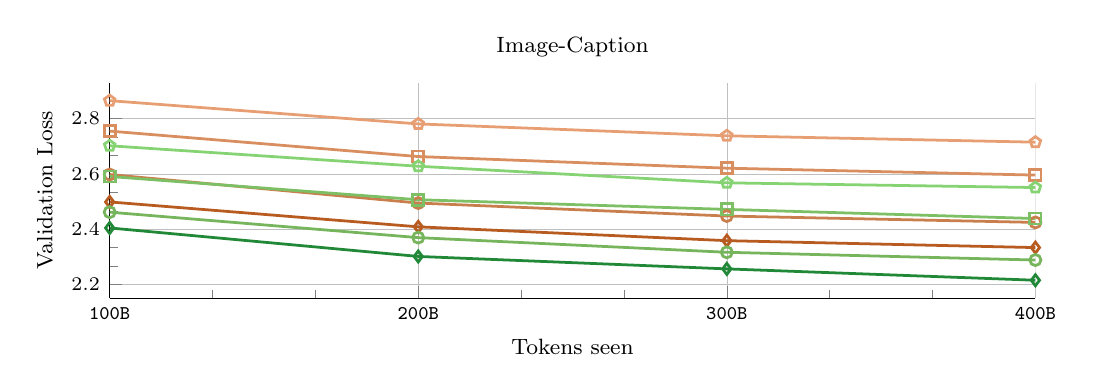
\begin{tikzpicture}
    \begin{axis}[
        legend pos=north east,
        grid=major,
        grid style={line width=.1pt, draw=gray!30},
        major grid style={line width=.2pt,draw=gray!50},
        minor tick num=2,
        axis x line*=bottom,
        axis y line*=left,
        xtick={
        0.1,
        0.2,
        0.3,
        0.4
        },
        xticklabels={
        \texttt{100B},
        \texttt{200B},
        \texttt{300B},
        \texttt{400B}
        },
        xmin=0.1,
        xmax=0.4,
        height=1.7in,
        width=1.1\linewidth,
        ylabel style={align=center, font=\small},
        xlabel style={font=\footnotesize},
        ylabel={\footnotesize{Validation Loss}},
        xlabel={\footnotesize{Tokens seen}},
        title={\footnotesize{Image-Caption}},
        ytick distance=0.2,
        yticklabel style={font=\scriptsize, /pgf/number format/fixed, /pgf/number format/precision=1},
        xticklabel style={font=\scriptsize},
        mark options={solid},
        legend style={cells={align=left}, font=\footnotesize, text=black},
        legend columns=6,
        legend cell align={left},
        legend to name=sharedlegend,
    ]

\addplot[legend early_0_2b style,mark=pentagon, mark size=2pt] plot coordinates {
        (0.05,2.95)
        (0.1, 2.865)
        (0.2, 2.781)
        (0.3, 2.738)
        (0.4, 2.715)

};
    \addplot[legend early_0_4b style,mark=square, mark size=2pt] plot coordinates {
        (0.05,2.852)
        (0.1, 2.755)
        (0.2, 2.663)
        (0.3, 2.621)
        (0.4, 2.596)

};
    \addplot[legend early_0_9b style,mark=o, mark size=2pt] plot coordinates {
    (0.05, 2.716)
    (0.1, 2.598)
    (0.2, 2.495)
    (0.3, 2.448)
    (0.4, 2.425)

};

    \addplot[legend early style,mark=diamond, mark size=2pt] plot coordinates {
        (0.05, 2.606)
        (0.1, 2.499)
        (0.2, 2.409)
        (0.3, 2.359)
        (0.4, 2.334)

    };

\addplot[legend moe_0_2b style,,mark=pentagon, mark size=2pt] plot coordinates {
        (0.05, 2.809)
        (0.1, 2.702)
        (0.2, 2.628)
        (0.3, 2.568)
        (0.4, 2.551)

    };

    \addplot[legend moe_0_4b style,,mark=square, mark size=2pt] plot coordinates {
        (0.05, 2.697)
        (0.1, 2.591)
        (0.2, 2.507)
        (0.3, 2.472)
        (0.4, 2.439)

    };

    \addplot[legend moe_0_9b style,,mark=o, mark size=2pt] plot coordinates {
        (0.05, 2.586)
        (0.1, 2.462)
        (0.2, 2.37)
        (0.3, 2.317)
        (0.4, 2.289)

    };

    \addplot[legend moe style,mark=diamond, mark size=2pt] plot coordinates {
        (0.05, 2.537)
        (0.1, 2.405)
        (0.2, 2.302)
        (0.3, 2.257)
        (0.4, 2.216)

    };

\end{axis}
\end{tikzpicture}

    \end{subfigure}
    \begin{subfigure}[t]{0.49\linewidth}
        
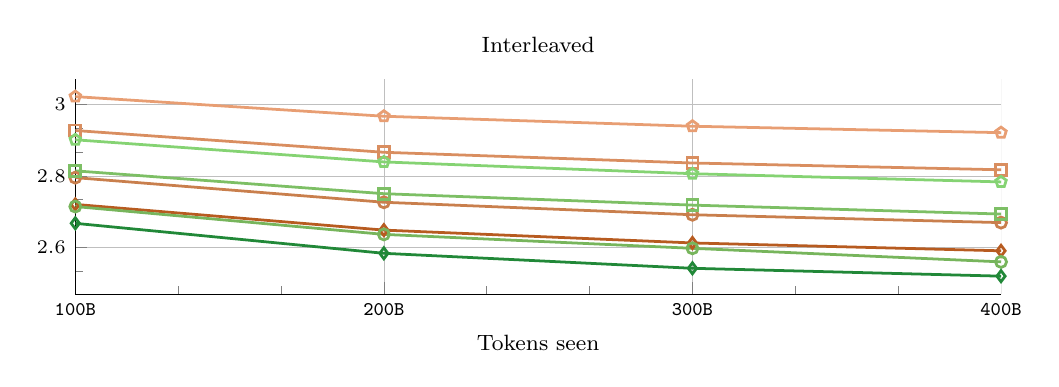
\begin{tikzpicture}
    \begin{axis}[
        legend pos=north east,
        grid=major, %
        grid style={line width=.1pt, draw=gray!30}, %
        major grid style={line width=.2pt,draw=gray!50},
        minor tick num=2,
        axis x line*=bottom,
        axis y line*=left,
        xtick={
        0.1, 
        0.2, 
        0.3,
        0.4
        },
        xticklabels={
        \texttt{100B}, 
        \texttt{200B}, 
        \texttt{300B},
        \texttt{400B}
        },
        xmin=0.1,
        xmax=0.4,
        height=1.7in,
        width=1.1\linewidth,
        ylabel style={align=center, font=\small},
        xlabel style={font=\footnotesize},
        xlabel={\footnotesize{Tokens seen}},
        title={\footnotesize{Interleaved}},
        ytick distance=0.2,
        yticklabel style={font=\scriptsize, /pgf/number format/fixed, /pgf/number format/precision=1},
        xticklabel style={font=\scriptsize},
        mark options={solid},
        legend style={cells={align=left}, font=\scriptsize, text=black}, %
        legend columns=4, %
        legend cell align={left},
        legend to name=sharedlegend,
    ]


    \addplot[legend early_0_2b style,mark=pentagon, mark size=2pt] plot coordinates {
        (0.05, 3.094)
        (0.1, 3.022)
        (0.2, 2.967)
        (0.3, 2.939)
        (0.4, 2.921)
    };
    \addlegendentry{\scalebox{0.85}{Dense-275M}}

    \addplot[legend early_0_4b style,mark=square, mark size=2pt] plot coordinates {
        (0.05, 2.998)
        (0.1, 2.927)
        (0.2, 2.866)
        (0.3, 2.836)
        (0.4, 2.817)
    };
    \addlegendentry{\scalebox{0.85}{Dense-464M}}


    \addplot[legend early_0_9b style,mark=o, mark size=2pt] plot coordinates {
        (0.05, 2.885)
        (0.1, 2.795)
        (0.2, 2.726)
        (0.3, 2.691)
        (0.4, 2.669)
    };
    \addlegendentry{\scalebox{0.85}{Dense-932M}}


    \addplot[legend early style,mark=diamond, mark size=2pt] plot coordinates {
        (0.05, 2.811)
        (0.1, 2.72)
        (0.2, 2.648)
        (0.3, 2.612)
        (0.4, 2.59)        
    };
    \addlegendentry{\scalebox{0.85}{Dense-1.6B}}

    

    

    \addplot[legend moe_0_2b style,mark=pentagon, mark size=2pt] plot coordinates {
        (0.05, 2.981)
        (0.1, 2.901)
        (0.2, 2.839)
        (0.3, 2.806)
        (0.4, 2.783)
    };
    \addlegendentry{\scalebox{0.85}{MoE-275M}}


    \addplot[legend moe_0_4b style,mark=square, mark size=2pt] plot coordinates {
        (0.05, 2.895)
        (0.1, 2.814)
        (0.2, 2.75)
        (0.3, 2.718)
        (0.4, 2.693)
    };
    \addlegendentry{\scalebox{0.85}{MoE-464M}}

    \addplot[legend moe_0_9b style,mark=o, mark size=2pt] plot coordinates {
        (0.05, 2.812)
        (0.1, 2.714)
        (0.2, 2.636)
        (0.3, 2.597)
        (0.4, 2.559)
    };
    \addlegendentry{\scalebox{0.85}{MoE-932M}}

    \addplot[legend moe style,mark=diamond, mark size=2pt] plot coordinates {
        (0.05, 2.77)
        (0.1, 2.667)
        (0.2, 2.583)
        (0.3, 2.541)
        (0.4, 2.519)
    };
    \addlegendentry{\scalebox{0.85}{MoE-1.63B}}





    \end{axis}
\end{tikzpicture}
    \end{subfigure}
    \vspace{-15pt}
    \begin{center}
        \ref{sharedlegend}
    \end{center}
    \caption{\textbf{MoE 与 稠密: 训练 FLOPs 的缩放。} 当同时扩展训练词元的数量和模型的大小时,我们比较了 MoE 和早期融合的稠密 模型。在匹配活跃参数数量时,MoE 超过了稠密模型。}
    \label{fig:dense_vs_moe_scaledata}
            
    \end{minipage}
    \hfill
    \begin{minipage}[t]{0.38\textwidth}
            \centering
    \captionsetup{type=figure}
    \begin{subfigure}[t]{1.0\linewidth}
        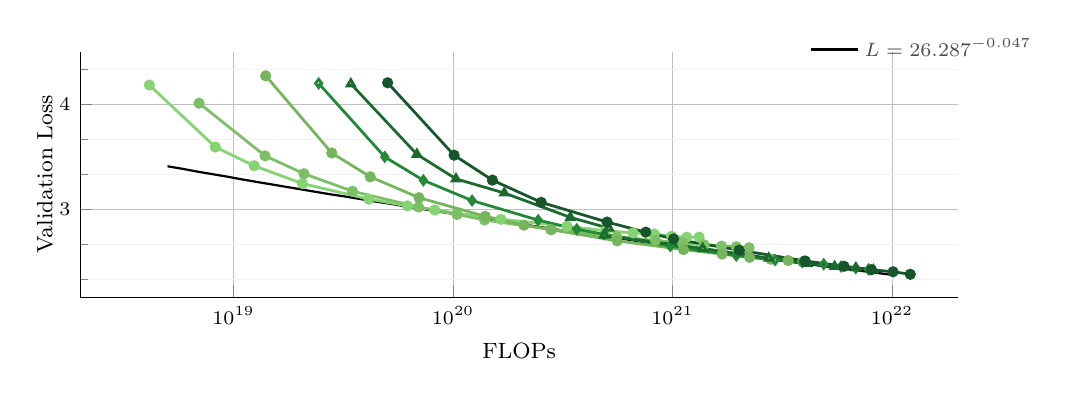
\begin{tikzpicture}
    \begin{axis}[
        legend pos=north east,
        grid=both,
        grid style={line width=.1pt, draw=gray!10},
        major grid style={line width=.2pt,draw=gray!50},
        minor tick num=2,
        axis x line*=bottom,
        axis y line*=left,
        xmode=log, %
        log basis x=10, %
        xtick={
            1E+19,
            1E+20,
            1E+21,
            1E+22
        },
        xmin=2E+18,
        xmax=2E+22,
        ymax=4.5,
        height=1.85in,
        width=1.05\linewidth,
        ylabel style={align=center, font=\scriptsize, yshift=-1ex},
        xlabel style={font=\scriptsize},
        ylabel={\footnotesize{Validation Loss}},
        xlabel={\footnotesize{FLOPs}},
        yticklabel style={font=\scriptsize},
        xticklabel style={font=\scriptsize},
        legend style={cells={align=left}, font=\scriptsize, fill opacity=0.7, fill=none, draw=none, at={(1.1, 1.1)}}, %
        mark options={solid},
    ]

        


    \addplot[color=black, thick, samples=50, domain=5e18:10e21] {26.287135104499598*x^(-0.04742807363789748)};
    \addlegendentry{$L = 26.287^{-0.047}$};


    
    



    \addplot[legend moe_0_2b style] plot coordinates {
        (4.13e+18, 4.182666666666666)
        (8.25e+18, 3.5933333333333333)
        (1.24e+19, 3.415333333333333)
        (2.06e+19, 3.2453333333333334)
        (4.13e+19, 3.098333333333333)
        (6.19e+19, 3.0340000000000003)
        (8.25e+19, 2.9949999999999997)
        (1.65e+20, 2.9066666666666663)
        (3.3e+20, 2.84)
        (4.95e+20, 2.798)
        (6.6e+20, 2.7773333333333334)
        (8.25e+20, 2.766666666666667)
        (9.9e+20, 2.7453333333333334)
        (1.16e+21, 2.736333333333333)
        (1.32e+21, 2.736666666666667)
    };
    \addplot[legend moe_0_4b style] plot coordinates {
        (6.96e+18, 4.010000000000001)
        (1.39e+19, 3.5096666666666665)
        (2.09e+19, 3.34)
        (3.48e+19, 3.173)
        (6.96e+19, 3.0226666666666664)
        (1.04e+20, 2.952666666666667)
        (1.39e+20, 2.899666666666667)
        (2.78e+20, 2.8106666666666666)
        (5.57e+20, 2.74)
        (8.35e+20, 2.7070000000000003)
        (1.11e+21, 2.6806666666666668)
        (1.39e+21, 2.6646666666666667)
        (1.67e+21, 2.651666666666667)
        (1.95e+21, 2.6460000000000004)
        (2.23e+21, 2.636)
    };
    \addplot[legend moe_0_9b style] plot coordinates {
        (1.4e+19, 4.270333333333333)
        (2.8e+19, 3.5366666666666666)
        (4.19e+19, 3.310333333333334)
        (6.99e+19, 3.112)
        (1.4e+20, 2.9346666666666663)
        (2.1e+20, 2.8510000000000004)
        (2.8e+20, 2.8073333333333337)
        (5.59e+20, 2.701333333333333)
        (1.12e+21, 2.6183333333333336)
        (1.68e+21, 2.5753333333333335)
        (2.24e+21, 2.5446666666666666)
        (2.8e+21, 2.5263333333333335)
        (3.36e+21, 2.514666666666667)
        (3.91e+21, 2.5003333333333333)
    };

    \addplot[legend moe style] plot coordinates {
        (2.44e+19, 4.198333333333333)
        (4.88e+19, 3.499333333333333)
        (7.32e+19, 3.2769999999999997)
        (1.22e+20, 3.0843333333333334)
        (2.44e+20, 2.8986666666666667)
        (3.66e+20, 2.8113333333333332)
        (4.88e+20, 2.764)
        (9.76e+20, 2.651333333333333)
        (1.95e+21, 2.5613333333333332)
        (2.93e+21, 2.5180000000000002)
        (3.9e+21, 2.5003333333333333)
        (4.88e+21, 2.4793333333333334)
        (5.86e+21, 2.4573333333333336)
        (6.83e+21, 2.4423333333333335)
        (7.81e+21, 2.4309999999999996)
    };

    \addplot[legend moe_2_2b style] plot coordinates {
        (3.42e+19, 4.194)
        (6.84e+19, 3.5239999999999996)
        (1.03e+20, 3.2906666666666666)
        (1.71e+20, 3.156333333333333)
        (3.42e+20, 2.9246666666666665)
        (5.13e+20, 2.821)
        (4.88e+20, 2.7543333333333333)
        (1.37e+21, 2.6296666666666666)
        (2.74e+21, 2.5369999999999995)
        (4.1e+21, 2.488)
        (5.47e+21, 2.458)
        (6.84e+21, 2.4436666666666667)
        (8.21e+21, 2.4246666666666665)
    };
    \addplot[legend moe_3_3b style] plot coordinates {
        (5.03e+19, 4.2043333333333335)
        (1.01e+20, 3.5156666666666667)
        (1.51e+20, 3.2786666666666666)
        (2.52e+20, 3.0673333333333335)
        (5.03e+20, 2.8800000000000003)
        (7.55e+20, 2.7840000000000003)
        (1.01e+21, 2.720333333333333)
        (2.01e+21, 2.613)
        (4.02e+21, 2.510333333333333)
        (6.04e+21, 2.46)
        (8.05e+21, 2.427)
        (1.01e+22, 2.40752)
        (1.21e+22, 2.3835766666666665)
    };
    

    \end{axis}
\end{tikzpicture}
    \end{subfigure}
    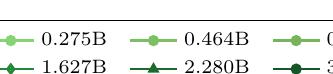
\begin{tikzpicture}
        \node[anchor=north] (legend) at (0\linewidth, 0) {
            \begin{axis}[
                        hide axis, %
                        xmin=0, xmax=0.5, ymin=0, ymax=1, %
                        legend columns=3, %
                        legend style={
                            at={(-0.14, -0.04)}, %
                            anchor=north, %
                            /tikz/every even column/.append style={column sep=0.2cm}, %
                            scale=0.5,
                            cells={align=left}, font=\scriptsize,
                            anchor=center,
                        },
                    ]
                \addlegendimage{legend moe_0_2b style}
                \addlegendentry{0.275B}
                \addlegendimage{legend moe_0_4b style}
                \addlegendentry{0.464B}
                \addlegendimage{legend moe_0_9b style}
                \addlegendentry{0.932B}
                \addlegendimage{legend moe style}
                \addlegendentry{1.627B}
                \addlegendimage{legend moe_2_2b style}
                \addlegendentry{2.280B}
                \addlegendimage{legend moe_3_3b style}
                \addlegendentry{3.354B}
            \end{axis}
        };
    \end{tikzpicture}
    \vspace{20pt}
    \caption{\textbf{稀疏早期融合NMM的缩放规律。} 我们报告最终的验证损失,该损失在交错的、图像-标题和文本数据上取平均值。}
    \label{fig:early_scaleflops_moe_avg}

    \end{minipage}
\end{figure}


\subsection{Emergence of expert specialization and sharing}
\label{sec:specialization}
We investigate multimodal specialization in MoE architectures. In~\cref{fig:tokens_assignment}, we visualize the normalized number of text and image tokens assigned to each expert across layers.  To quantify this specialization, we compute a specialization score, defined as the average, across all experts within a layer, of $1-H(p)$, where $H$ is the binary entropy of each expert's text/image token distribution. We plot this specialization score in~\cref{fig:tokens_specialization}.  Higher specialization scores indicate a tendency for experts to focus on either text or image tokens, while lower scores indicate a shared behavior.  These visualizations provide clear evidence of modality-specific experts, particularly in the early layers. Furthermore, the specialization score decreases as the number of layers increases, before rising again in the last layers. This suggests that early and final layers exhibit higher modality specialization compared to mid-layers. This behavior is intuitive, as middle layers are expected to hold higher-level features that may generalize across modalities, \edit{and consistent with findings in \citep{shukor2024implicit} that shows increasing alignment between modalities across layers}. The emergence of both expert specialization and cross-modality sharing in our modality-agnostic MoE, suggests it may be a preferable approach compared to modality-aware sparsity. All data displayed here is from an early-fusion MoE model with 1B active parameters trained for 300B tokens. 






\begin{table}[h!]
    \centering
    \setlength{\tabcolsep}{12pt} %
    \renewcommand{\arraystretch}{1} %
    \resizebox{1\linewidth}{!}{
    \begin{tabular}{lcccccccc}
        & \multicolumn{6}{c}{Accuracy} & \multicolumn{2}{c}{CIDEr}  \\
        \cmidrule(lr){2-7} \cmidrule(lr){8-9}
        & AVG & VQAv2 & TextVQA & OKVQA & GQA & VizWiz & COCO & TextCaps \\
        \shline
        Late-fusion   & 46.8  & 69.4  & 25.8  & 50.1  & \textbf{65.8}  & 22.8  & 70.7  & 50.9 \\
        Early-fusion  & 47.6  & 69.3  & 28.1  & \textbf{52.1}  & 65.4  & 23.2  & \textbf{72.0}  & 53.8 \\
        Early-MoEs    & \textbf{48.2}  & \textbf{69.8}  & \textbf{30.0}  & \textbf{52.1}  & 65.4  & \textbf{23.6}  & 69.6  & \textbf{55.7} \\
    \end{tabular}%
    }
    \caption{\textbf{在LLaVA混合数据上的监督微调。} 所有模型原生规模为1.5B,已在300B词元上预训练。}
    \vspace{-7pt}
    \label{tab:sft}
\end{table}


\vspace{-1cm}
\section{Evaluation on downstream tasks with SFT} 
Following previous work on scaling laws, we primarily rely on validation losses. However, we generally find that this evaluation correlates well
with performance on downstream tasks. To validate this, we conduct a multimodal
instruction tuning stage (SFT) on the LLaVA mixture \citep{liu2024improvedllava} and report
accuracy and CIDEr scores across several VQA and captioning tasks.
\cref{tab:sft} confirms the ranking of different model configurations.
Specifically, early fusion outperforms late fusion, and MoEs outperform dense
models. However, since the models are relatively small (1.5B scale), trained
from scratch, and fine-tuned on a small dataset, the overall scores
are lower than the current state of the art.  Further implementation
details can be found in~\Cref{app:implementation_details}.  


\begin{figure}[t!]
    \begin{minipage}[t]{0.58\textwidth}
        \centering
    \captionsetup{type=figure}
    \begin{subfigure}[t]{0.49\linewidth}
        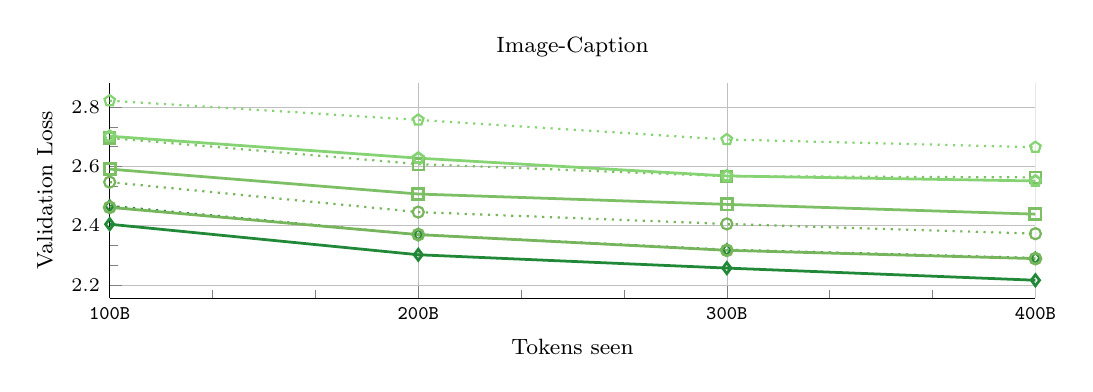
\begin{tikzpicture}
    \begin{axis}[
        legend pos=north east,
        grid=major,
        grid style={line width=.1pt, draw=gray!30},
        major grid style={line width=.2pt,draw=gray!50},
        minor tick num=2,
        axis x line*=bottom,
        axis y line*=left,
        xtick={
        0.1,
        0.2,
        0.3,
        0.4
        },
        xticklabels={
        \texttt{100B},
        \texttt{200B},
        \texttt{300B},
        \texttt{400B}
        },
        xmin=0.1,
        xmax=0.4,
        height=1.7in,
        width=1.1\linewidth,
        ylabel style={align=center, font=\small},
        xlabel style={font=\footnotesize},
        ylabel={\footnotesize{Validation Loss}},
        xlabel={\footnotesize{Tokens seen}},
        title={\footnotesize{Image-Caption}},
        ytick distance=0.2,
        yticklabel style={font=\scriptsize, /pgf/number format/fixed, /pgf/number format/precision=1},
        xticklabel style={font=\scriptsize},
        mark options={solid},
        legend style={cells={align=left}, font=\footnotesize, text=black},
        legend columns=6,
        legend cell align={left},
        legend to name=sharedlegend,
    ]

\addplot[legend moe_0_2b style,thick, dotted, mark=pentagon, mark size=2pt] plot coordinates {
        (0.1, 2.822)
        (0.2, 2.757)
        (0.3, 2.691)
        (0.4, 2.665)
    };
    \addplot[legend moe_0_4b style,thick, dotted, mark=square, mark size=2pt] plot coordinates {
        (0.1, 2.696)
        (0.2, 2.608)
        (0.3, 2.567)
        (0.4, 2.563)
    };
    \addplot[legend moe_0_9b style, thick, dotted, mark=o, mark size=2pt] plot coordinates {
        (0.1, 2.547)
        (0.2, 2.446)
        (0.3, 2.406)
        (0.4, 2.373)
    };

    \addplot[legend moe style, thick, dotted, mark=diamond, mark size=2pt] plot coordinates {
        (0.1, 2.467)
        (0.2, 2.37)
        (0.3, 2.319)
        (0.4, 2.291)

    };

\addplot[legend moe_0_2b style,mark=pentagon, mark size=2pt] plot coordinates {
        (0.05, 2.809)
        (0.1, 2.702)
        (0.2, 2.628)
        (0.3, 2.568)
        (0.4, 2.551)

    };

    \addplot[legend moe_0_4b style,mark=square, mark size=2pt] plot coordinates {
        (0.05, 2.697)
        (0.1, 2.591)
        (0.2, 2.507)
        (0.3, 2.472)
        (0.4, 2.439)

    };

    \addplot[legend moe_0_9b style,mark=o, mark size=2pt] plot coordinates {
        (0.05, 2.586)
        (0.1, 2.462)
        (0.2, 2.37)
        (0.3, 2.317)
        (0.4, 2.289)

    };

    \addplot[legend moe style,mark=diamond, mark size=2pt] plot coordinates {
        (0.05, 2.537)
        (0.1, 2.405)
        (0.2, 2.302)
        (0.3, 2.257)
        (0.4, 2.216)

    };

\end{axis}
\end{tikzpicture}

    \end{subfigure}
    \begin{subfigure}[t]{0.49\linewidth}
        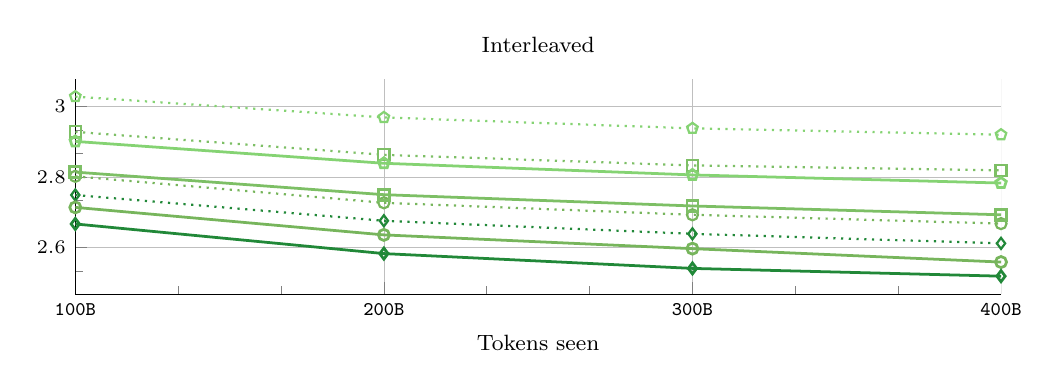
\begin{tikzpicture}
    \begin{axis}[
        legend pos=north east,
        grid=major,
        grid style={line width=.1pt, draw=gray!30},
        major grid style={line width=.2pt,draw=gray!50},
        minor tick num=2,
        axis x line*=bottom,
        axis y line*=left,
        xtick={
        0.1,
        0.2,
        0.3,
        0.4
        },
        xticklabels={
        \texttt{100B},
        \texttt{200B},
        \texttt{300B},
        \texttt{400B}
        },
        xmin=0.1,
        xmax=0.4,
        height=1.7in,
        width=1.1\linewidth,
        ylabel style={align=center, font=\small},
        xlabel style={font=\footnotesize},
        xlabel={\footnotesize{Tokens seen}},
        title={\footnotesize{Interleaved}},
        ytick distance=0.2,
        yticklabel style={font=\scriptsize, /pgf/number format/fixed, /pgf/number format/precision=1},
        xticklabel style={font=\scriptsize},
        mark options={solid},
        legend style={cells={align=left}, font=\scriptsize, text=black, mark options=solid},
        legend columns=4,
        legend cell align={left},
        legend to name=sharedlegend,
    ]

\addplot[legend moe_0_2b style,thick, dotted, mark=pentagon, mark size=2pt] plot coordinates {
        (0.1, 3.028)
        (0.2, 2.969)
        (0.3, 2.938)
        (0.4, 2.92)
    };
    \addlegendentry{\scalebox{0.8}{Aware-275M}}

    \addplot[legend moe_0_4b style,thick, dotted, mark=square, mark size=2pt] plot coordinates {
        (0.1, 2.928)
        (0.2, 2.863)
        (0.3, 2.833)
        (0.4, 2.819)
    };
    \addlegendentry{\scalebox{0.8}{Aware-464M}}

    \addplot[legend moe_0_9b style, thick, dotted, mark=o, mark size=2pt] plot coordinates {
        (0.1, 2.802)
        (0.2, 2.727)
        (0.3, 2.693)
        (0.4, 2.668)
    };
    \addlegendentry{\scalebox{0.8}{Aware-932M}}

    \addplot[legend moe style, thick, dotted, mark=diamond, mark size=2pt] plot coordinates {
        (0.1, 2.749)
        (0.2, 2.676)
        (0.3, 2.639)
        (0.4, 2.612)
    };
    \addlegendentry{\scalebox{0.8}{Aware-1.63}}

\addplot[legend moe_0_2b style,mark=pentagon, mark size=2pt] plot coordinates {
        (0.05, 2.981)
        (0.1, 2.901)
        (0.2, 2.839)
        (0.3, 2.806)
        (0.4, 2.783)
    };
    \addlegendentry{\scalebox{0.8}{Agnostic-275M}}

\addplot[legend moe_0_4b style,mark=square, mark size=2pt] plot coordinates {
        (0.05, 2.895)
        (0.1, 2.814)
        (0.2, 2.75)
        (0.3, 2.718)
        (0.4, 2.693)
    };
    \addlegendentry{\scalebox{0.8}{Agnostic-464M}}

    \addplot[legend moe_0_9b style,mark=o, mark size=2pt] plot coordinates {
        (0.05, 2.812)
        (0.1, 2.714)
        (0.2, 2.636)
        (0.3, 2.597)
        (0.4, 2.559)
    };
    \addlegendentry{\scalebox{0.8}{Agnostic-932M}}

    \addplot[legend moe style,mark=diamond, mark size=2pt] plot coordinates {
        (0.05, 2.77)
        (0.1, 2.667)
        (0.2, 2.583)
        (0.3, 2.541)
        (0.4, 2.519)
    };
    \addlegendentry{\scalebox{0.8}{Agnostic-1.63B}}

\end{axis}
\end{tikzpicture}

    \end{subfigure}
    \vspace{-15pt}
    \begin{center}
        \ref{sharedlegend}
    \end{center}

\caption{\textbf{基于模态感知与无关模态路由的稀疏NMM比较。} 我们在扩大训练标记数量和模型规模时,比较了无关模态路由与基于模态感知路由的性能。}
    \label{fig:hard_vs_moe_scaledata}

    \end{minipage}
    \hfill
    \begin{minipage}[t]{0.38\textwidth}
        \centering
\captionsetup{type=figure}

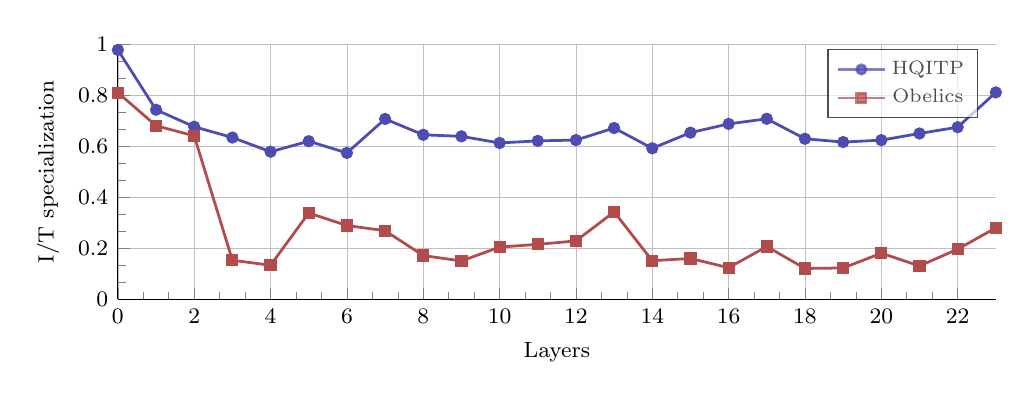
\begin{tikzpicture}
\begin{axis}[
    grid=major,
    grid style={line width=.1pt, draw=gray!30},
    major grid style={line width=.2pt,draw=gray!50},
    minor tick num=2,
    axis x line*=bottom,
    axis y line*=left,
    xmin=0,
    xmax=23,
    ymin=0.0,
    ymax=1.0,
    height=1.9in,
    width=1.05\linewidth,
    ylabel style={align=center, font=\footnotesize},
    xlabel style={font=\footnotesize},
    ylabel=\footnotesize{I/T specialization},
    xlabel={\footnotesize{Layers}},
    ytick distance=0.2,
    yticklabel style={font=\footnotesize, /pgf/number format/fixed, /pgf/number format/precision=2},
    xticklabel style={font=\footnotesize},
    xtick={0,2,4,6,8,10,12,14,16,18,20,22},
    xticklabels={0,2,4,6,8,10,12,14,16,18,20,22},
    mark options={solid},
    legend style={cells={align=left}, font=\scriptsize, text=black, opacity=0.7},
]

\addplot[color=blue!40!gray, mark=*, mark size=1.7pt, line width=1pt] plot coordinates {
(0, 0.9769479348349329)
(1, 0.7427025603097698)
(2, 0.6762374582380828)
(3, 0.6340138224507533)
(4, 0.5783047019889138)
(5, 0.6195673358863271)
(6, 0.5737861572855565)
(7, 0.7066104505575633)
(8, 0.6446960774170309)
(9, 0.6386074080824291)
(10, 0.6128197724774395)
(11, 0.620867456928868)
(12, 0.6240480502092688)
(13, 0.6712385178771478)
(14, 0.591805441066985)
(15, 0.6531511085896324)
(16, 0.6873617200378165)
(17, 0.7072043647262733)
(18, 0.6290614078343542)
(19, 0.6162376387022552)
(20, 0.6237776803436119)
(21, 0.649774290665718)
(22, 0.6745086003424091)
(23, 0.810597818982423)
};
\addlegendentry{HQITP}

\addplot[color=red!40!gray, mark=square*, mark size=1.7pt, line width=1pt] plot coordinates {
(0, 0.8098464848229123)
(1, 0.6803114998878562)
(2, 0.640428138604904)
(3, 0.15356616480436047)
(4, 0.13402442087930844)
(5, 0.33860156581505885)
(6, 0.2894806232076399)
(7, 0.269278406260023)
(8, 0.17195894943324286)
(9, 0.15091557473173656)
(10, 0.2050356661788283)
(11, 0.21603190628094793)
(12, 0.22923064654990588)
(13, 0.34291773221125066)
(14, 0.15175535984919586)
(15, 0.16059145647036643)
(16, 0.12438172525723101)
(17, 0.20722842981400202)
(18, 0.12145399323126793)
(19, 0.12335098001817868)
(20, 0.1811717532056517)
(21, 0.13129565163316004)
(22, 0.19701360887683683)
(23, 0.28035775702112686)
};
\addlegendentry{Obelics}
\end{axis}

\end{tikzpicture}

\caption{\textbf{MoE 专门化.} 基于熵的图像/文本专门化(见~\cref{sec:specialization})在两个数据源:HQITP 和 Obelics 的各层之间的变化。
\edit{两个数据源都表现出类似的趋势:在早期层中得分下降,随后在最后几层中再次上升.}}
\label{fig:tokens_specialization}

    \end{minipage}
    \vspace{3mm}
\end{figure}


\section{Related Work}
\label{sec:related_work}

In this section, we review areas mostly related to our work, \ie, image retrieval and visual place recognition.

\subsection{Image Retrieval}

Image retrieval is a fundamental and well-established task in computer vision that involves searching for images similar to a given query within a large database.
The process of image retrieval typically consists of two stages: global retrieval and re-ranking. In the first stage, a global descriptor that aggregates local features is used to retrieve $k$ candidates from a large database. This is followed by spatial verification through local feature matching to re-rank these $k$ candidates. Early research relied on handcrafted features \cite{Lowe2004DistinctiveIF, BAY2008346}, while current methods utilize deep networks to learn informative representations \cite{cao2020unifyingdeeplocalglobal, radenović2018finetuningcnnimageretrieval}.

Most image retrieval methods focus on selecting diverse relevant images to help users discover options that align with their interests or needs in real-world applications \cite{Wan2014DeepLF}. Although these methods are effective in retrieving similar images, they often lack the emphasis on distinguishing between categories or achieving precise ReID \cite{10.1145/1348246.1348248}.
In \mbox{contrast}, our approach prioritizes achieving accurate ReID. Following a ``global retrieval and re-ranking" pipeline, we first use global context features to identify the top five room candidates. Our object-aware mechanism then refines the search in a coarse-to-fine manner, progressively distinguishing among candidates until the most similar room is \mbox{identified}, yielding accurate results.

\begin{figure*}[ht]
    \centering
    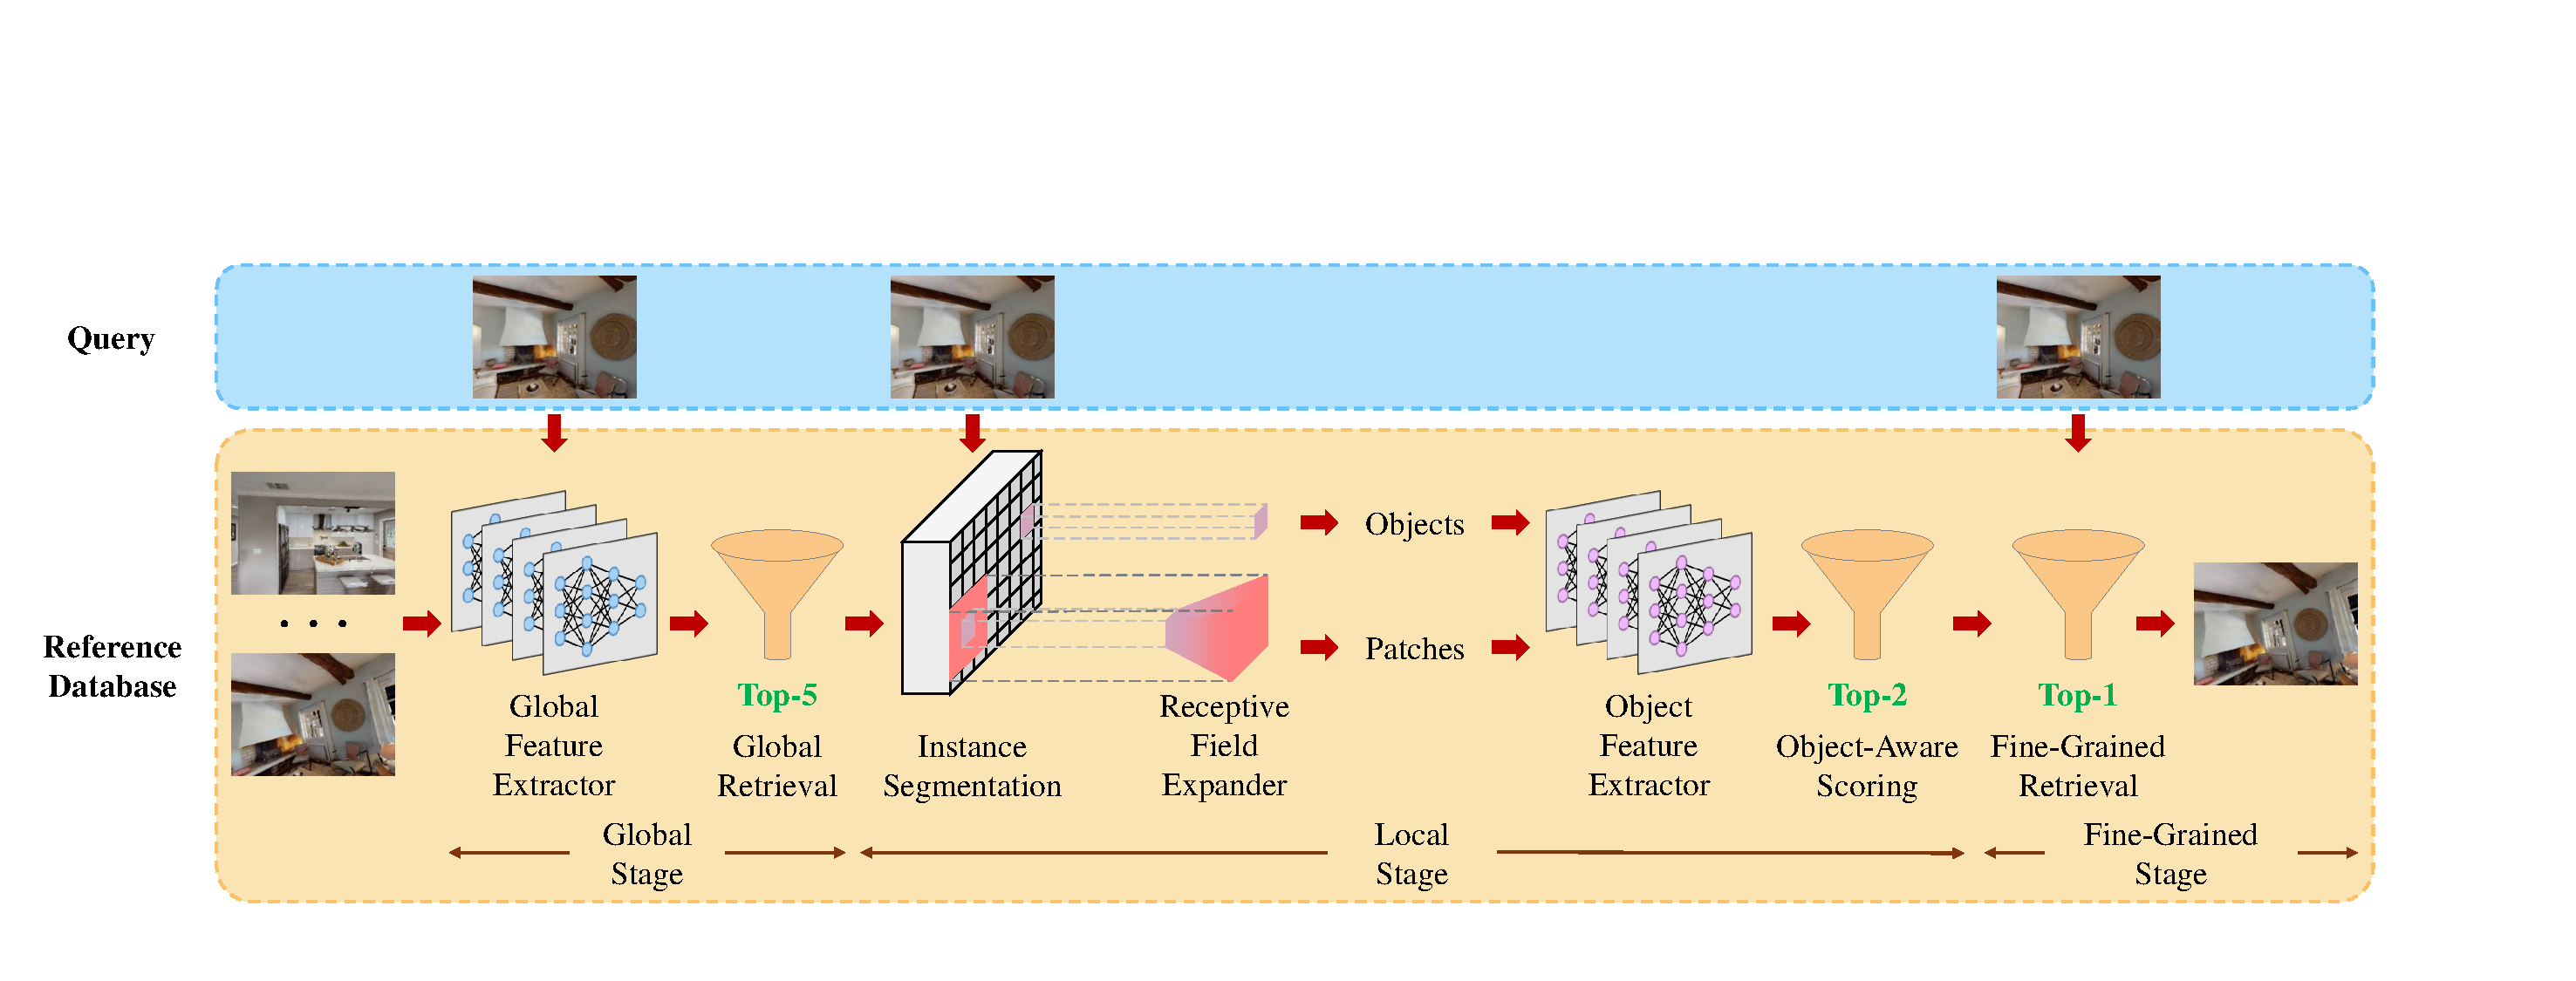
\includegraphics[width=\textwidth]{pipeline_font.pdf}
    \vspace{-16pt}
    \caption{\textbf{The AirRoom coarse-to-fine pipeline}. The pipeline begins with the Global Feature Extractor, which captures global context features to retrieve the top-5 reference images. Instance segmentation then generates object masks, followed by the Receptive Field Expander, which extracts object patches. The Object Feature Extractor processes both object and patch features. The Object-Aware Scoring module narrows the selection to the top-2 candidates, and Fine-Grained Retrieval identifies the most suitable reference image.}
    \vspace{-15pt}
    \label{fig:pipeline}
\end{figure*}

\subsection{Visual Place Recognition}

Visual place recognition (VPR) is often framed as a special image retrieval problem, aiming to match a view of a location with an image of the same place taken under different conditions.
Previous methods fall into two categories: those that directly use global descriptors and those that aggregate local features into a global descriptor. Earlier approaches that relied on global descriptors primarily used CNN-based backbones, such as ResNet \cite{he2015deepresiduallearningimage}, to generate these descriptors. More recent methods, however, leverage foundation models like DINOv2 \cite{oquab2024dinov2learningrobustvisual} for enhanced feature representation. In the aggregation category, early techniques employed handcrafted features like SIFT \cite{Lowe2004DistinctiveIF}, SURF \cite{10.1007/11744023_32}, and ORB \cite{6126544}. Later advancements, including the NetVLAD series \cite{arandjelović2016netvladcnnarchitectureweakly, hausler2021patchnetvladmultiscalefusionlocallyglobal} and AnyLoc \cite{keetha2023anylocuniversalvisualplace}, adopted learning-based models to extract feature maps and combine local features into comprehensive global descriptors.

However, the high performance of most VPR approaches is largely attributed to large-scale training on VPR-specific datasets \cite{keetha2023anylocuniversalvisualplace}. Collecting extensive data for outdoor scenes is relatively straightforward due to natural variations in daylight, weather, and seasons. However, such data collection is more challenging in indoor rooms, making large-scale training on indoor datasets difficult and potentially limiting their effectiveness.
Our approach effectively tackles this challenge by focusing on object-oriented feature representations, allowing us to leverage mature, pre-trained models for object feature learning. This design enables AirRoom to deliver robust performance without requiring any additional training or fine-tuning on specific datasets.
% Our approach addresses this challenge by centering on objects within indoor spaces, leveraging object-related feature representations. Additionally, AirRoom benefits from mature, pre-trained models for object-centric feature learning. This design enables our approach to deliver robust performance without the need for additional training or fine-tuning on specific datasets.


\section{\edit{讨论和 }局限性} 

\cpar{\edit{多模态数据混合的缩放定律。}} 我们的缩放定律研究涵盖了不同的模型配置和训练混合。虽然结果表明缩放定律系数在混合中基本保持一致,但仍需要更广泛的混合变化探索来验证这一观察,并建立一个统一的缩放定律来考虑这个因素。  

\cpar{\edit{缩放定律和下游任务性能。} 与之前的缩放定律研究类似,我们的分析集中在通过验证损失衡量的预训练性能上。然而,这些发现转化为下游性能的程度仍然是一个开放的问题,需要进一步研究。}

\cpar{\edit{外推法到更大的规模。}} 缩放定律的预测准确率随着FLOPs的增加而提高~\cref{app:scaling_laws}。
\edit{此外,我们在外推到更大的模型大小时验证了我们的定律(\cref{sec:scaling_laws_evaluation})。} 然而,这些定律是否可以可靠地外推到极大规模的模型仍然是一个悬而未决的问题。 

\cpar{\edit{高分辨率和早期融合模型。} 使用高分辨率输入训练早期融合模型会导致视觉词元数量显著增加。虽然池化技术已被广泛应用于晚期融合模型,但对于早期融合可能需要替代方法。\edit{鉴于早期融合模型与大型语言模型的相似性,扩展上下文长度的技术似乎是有益的。}}

\cpar{\edit{多模态MoE模型的缩放规律。}} 对于MoE,我们仅考虑一种配置(顶级-1路由,8个专家)。\edit{我们发现此配置在我们的设置中表现合理,并遵循标准的MoE实现。}然而,当优化MoE架构或探索不同的负载均衡、路由策略以及不同专家实现时,结果可能会有所不同。\edit{更多}

\section{结论} 
我们探索了针对本地多模态模型进行计算最优预训练的各种策略。我们发现,NMM(神经多模态模型)遵循与LLM(大型语言模型)相似的缩放定律。与普遍的看法相反,我们发现在早期融合架构和晚期融合架构之间没有固有的优势。虽然这两种架构表现出相似的缩放特性,但早期融合模型更易于训练,并在较低的计算预算下优于晚期融合模型。此外,我们展示了稀疏架构能够鼓励模态特定的特化,从而在保持相同的推理成本的同时提高性能。




\section*{\edit{致谢}} 我们要感谢Philipp Dufter、Samira Abnar、Xiujun Li、Zhe Gan、Alexander Toshev、Yinfei Yang、Dan Busbridge和Jason Ramapuram进行了许多富有成果的讨论。我们要感谢Denise Hui和Samy Bengio在基础设施和计算方面的支持。最后,我们要感谢Louis Béthune、Pierre Ablin、Marco Cuturi以及Apple的MLR团队在整个项目中的支持。
{
    \small
    \bibliographystyle{ieeenat_fullname}
    \bibliography{main}
}
\clearpage
\appendix
\addcontentsline{toc}{section}{附录}
\renewcommand\ptctitle{Appendices}
\part{}
\parttoc
\clearpage
\clearpage
\setcounter{page}{1}
\maketitlesupplementary

\section{Datasets}
Table \ref{tab:MPReID} presents the composition of MPReID, while Table \ref{tab:HMReID}, Table \ref{tab:GibsonReID}, and Table \ref{tab:ReplicaReID} outline the compositions of HMReID, GibsonReID, and ReplicaReID, respectively. Table \ref{tab:Statistics} reports the number of semantically different rooms in each room ReID dataset.

\begin{table}[ht]
\centering
\vspace{-3pt}
\resizebox{\columnwidth}{!}{
\begin{tabular}{c|c|c|c|c|c}
\toprule
\textbf{Scene} & \textbf{Rooms} & \textbf{Images} & \textbf{Scene} & \textbf{Rooms} & \textbf{Images} \\
\midrule
8WUmhLawc2A & 8 & 1232 & EDJbREhghzL & 7 & 1078 \\
RPmz2sHmrrY & 5 & 770 & S9hNv5qa7GM & 9 & 1423 \\
ULsKaCPVFJR & 5 & 780 & VzqfbhrpDEA & 7 & 1078 \\
WYY7iVyf5p8 & 4 & 616 & X7HyMhZNoso & 7 & 1078 \\
YFuZgdQ5vWj & 7 & 1078 & i5noydFURQK & 7 & 1078 \\
jh4fc5c5qoQ & 5 & 770 & mJXqzFtmKg4 & 9 & 1386 \\
qoiz87JEwZ2 & 8 & 1232 & wc2JMjhGNzB & 11 & 1708 \\
yqstnuAEVhm & 6 & 924 & \textbf{Total} & \textbf{105} & \textbf{16231} \\
\bottomrule
\end{tabular}
}
\vspace{-1em}
\caption{Composition of MPReID.}
\label{tab:MPReID}
\end{table}

\vspace{-1em}

\begin{table}[ht]
\centering
\resizebox{\columnwidth}{!}{
\begin{tabular}{c|c|c|c|c|c}
\toprule
\textbf{Scene} & \textbf{Rooms} & \textbf{Images} & \textbf{Scene} & \textbf{Rooms} & \textbf{Images} \\
\midrule
7dmR22gwQpH & 6 & 924 & ACZZiU6BXLz & 5 & 682 \\
CETmJJqkhcK & 5 & 813 & CFVBbU9Rsyb & 5 & 770 \\
Coer9RdivP7 & 3 & 462 & DZsJKHoqEYg & 5 & 793 \\
EQSguCqe5Rk & 5 & 819 & Fgtk7tL8R9Y & 5 & 822 \\
GLAQ4DNUx5U & 7 & 1156 & GcfUJ79xCZc & 5 & 572 \\
NcK5aACg44h & 5 & 754 & P8L1328HrLi & 5 & 819 \\
VSxVP19Cdyw & 5 & 769 & b3CuYvwpzZv & 5 & 690 \\
ixTj1aTMup2 & 5 & 757 & ochRmQAHtkF & 5 & 641 \\
qWb4MVxqCW7 & 6 & 879 & rrjjmoZhZCo & 5 & 704 \\
w7QyjJ3H9Bp & 5 & 692 & zR6kPe1PsyS & 5 & 803 \\
zepmXAdrpjR & 3 & 460 & \textbf{Total} & \textbf{105} & \textbf{15781} \\
\bottomrule
\end{tabular}
}
\vspace{-1em}
\caption{Composition of HMReID.}
\label{tab:HMReID}
\end{table}

\vspace{-1em}

\begin{table}[ht]
\centering
\resizebox{\columnwidth}{!}{
\begin{tabular}{c|c|c|c|c|c}
\toprule
\textbf{Scene} & \textbf{Rooms} & \textbf{Images} & \textbf{Scene} & \textbf{Rooms} & \textbf{Images} \\
\midrule
Ackermanville & 1 & 154 & Angiola & 1 & 154 \\
Avonia & 2 & 308 & Beach & 3 & 462 \\
Branford & 1 & 154 & Brevort & 1 & 154 \\
Cason & 2 & 262 & Cooperstown & 2 & 308 \\
Corder & 2 & 308 & Creede & 4 & 526 \\
Elmira & 2 & 308 & Eudora & 2 & 308 \\
Fredericksburg & 2 & 308 & Greigsville & 1 & 154 \\
Idanha & 1 & 154 & Laytonsville & 3 & 462 \\
Lynxville & 2 & 308 & Mahtomedi & 2 & 257 \\
Mayesville & 2 & 308 & Northgate & 1 & 154 \\
Ogilvie & 2 & 308 & Ophir & 3 & 462 \\
Pablo & 1 & 154 & Sumas & 2 & 308 \\
- & - & - & \textbf{Total} & \textbf{45} & \textbf{6743} \\
\bottomrule
\end{tabular}
}
\vspace{-1em}
\caption{Composition of GibsonReID.}
\label{tab:GibsonReID}
\end{table}

\vspace{-1em}

\begin{table}[ht]
\centering
\resizebox{\columnwidth}{!}{
\begin{tabular}{c|c|c|c|c|c}
\toprule
\textbf{Scene} & \textbf{Rooms} & \textbf{Images} & \textbf{Scene} & \textbf{Rooms} & \textbf{Images} \\
\midrule
apartment\_0 & 3 & 462 & apartment\_1 & 1 & 154 \\
apartment\_2 & 4 & 616 & frl\_apartment\_0 & 3 & 426 \\
hotel\_0 & 1 & 154 & office\_0 & 1 & 154 \\
office\_2 & 1 & 140 & office\_3 & 1 & 140 \\
office\_4 & 1 & 154 & room\_0 & 1 & 154 \\
room\_1 & 1 & 154 & room\_2 & 1 & 154 \\
- & - & - & \textbf{Total} & \textbf{19} & \textbf{2862} \\
\bottomrule
\end{tabular}
}
\vspace{-1em}
\caption{Composition of ReplicaReID.}
\label{tab:ReplicaReID}
\end{table}

\begin{table}[h]
% \vspace{-10pt}
\centering
\resizebox{\columnwidth}{!}{
\begin{tabular}{c|c|c|c|c|c|c|c|c|c|c|c|c|c|c}
\hline
 & bathroom & kitchen & living & office & bedroom & theater & dining & wardrobe & gym & laundry & garage & storage & nursery & supermarket \\
\hline
MPReID & 13 & 13 & 20 & 3 & 41 & 4 & 4 & 2 & 2 & 2 & 1 & 0 & 0 & 0 \\
\hline
HMReID & 10 & 18 & 29 & 8 & 31 & 0 & 3 & 1 & 0 & 1 & 0 & 2 & 2 & 0 \\
\hline
GibsonReID & 2 & 10 & 11 & 3 & 12 & 0 & 1 & 0 & 3 & 1 & 0 & 1 & 0 & 1 \\
\hline
ReplicaReID & 0 & 2 & 6 & 6 & 3 & 0 & 2 & 0 & 0 & 0 & 0 & 0 & 0 & 0 \\
\hline
\end{tabular}
}
\caption{Statistics of semantically different rooms across four newly constructed room ReID datasets.}
\label{tab:Statistics}
% \vspace{-13pt}
\end{table}

\section{Experimental Details}

\subsection{Overall Performance Comparison}
\label{sec:appendix_overall}

\paragraph{Baseline Configuration} For CVNet, we use ResNet50 as the backbone and set the reduction dimension to 2048. For DINOv2, we utilize the DINOv2-Base checkpoint. For Patch-NetVLAD, we load pre-trained weights optimized on the Pittsburgh dataset, apply WPCA to reduce feature embedding dimensionality to 4096, set RANSAC as the matcher, use patch weights of 0.45, 0.15, and 0.4, configure patch sizes to 2, 5, and 8 with strides of 1 for all. For AnyLoc, we adopt AnyLoc-VLAD-DINOv2 with the DINOv2 ViT-G/14 architecture, set the descriptor layer to 31, use VLAD with 32 clusters, and specify the domain as \mbox{indoor}.

\paragraph{Baseline Adaptation} For CVNet and Patch-NetVLAD, we perform global retrieval by selecting the top-5 candidates, followed by re-ranking. For CVNet, the candidate with the highest CVNet-Rerank image similarity score is chosen as the final result, while for Patch-NetVLAD, the reference with the highest RANSAC score in the Pairwise Local Matching stage is selected. For DINOv2 and AnyLoc, global features are extracted from the query and reference images, and cosine similarity is computed. The reference image with the highest cosine similarity score is selected as the final match.

\paragraph{AirRoom Configuration} For the Global Feature Extractor, we use AnyLoc-VLAD-DINOv2 with the DINOv2 ViT-G/14 architecture, setting the descriptor layer to 31, applying VLAD with 32 clusters, and specifying the domain as indoor. For Instance Segmentation, we employ Semantic-SAM with pre-trained weights from SA-1B and a SwinL backbone. The Object Feature Extractor is implemented using a ResNet50 model pre-trained on the ImageNet dataset. For Fine-Grained Retrieval, we use LightGlue with the maximum number of keypoints set to 2048.

\subsection{Group-Wise Performance Comparison}

\paragraph{Baseline Configuration} For the ResNet50 backbone group, the configurations for ResNet50 and CVNet follow those detailed in \sref{sec:appendix_overall}. For the NetVLAD backbone group, we use NetVLAD with VGG-16 as the feature extractor, configured with 64 clusters and a feature dimensionality of 512. For Patch-NetVLAD, the feature dimensionalities are set to 4096, 512, and 128, respectively, with all other settings consistent with \sref{sec:appendix_overall}.

\paragraph{Baseline Adaptation} For the ResNet50 backbone group, ResNet50 extracts global features from the query and reference images, with cosine similarity used to select the reference image with the highest score as the final match. The adaptation for CVNet is detailed in \sref{sec:appendix_overall}. For the NetVLAD backbone group, NetVLAD aggregates global descriptors from the query and reference local features, and the reference with the highest cosine similarity score is chosen as the final result. The adaptation for Patch-NetVLAD also follows \sref{sec:appendix_overall}.

\paragraph{AirRoom Configuration} For the ResNet50 backbone group, ResNet50 is used as the Global Feature Extractor, with the configuration consistent with \sref{sec:appendix_overall}. For the NetVLAD backbone group, NetVLAD is used as the Global Feature Extractor, following the configuration outlined in the Baseline Configuration paragraph in this section. The configurations for the remaining modules in both groups are also consistent with \sref{sec:appendix_overall}.

\subsection{Pipeline Flexibility Evaluation}

\subsubsection{Global Feature Extractor}

\paragraph{Baseline Configuration} For ViT, we use the Base variant with a patch size of 16 and an input image size of 224×224, loading pre-trained weights from ImageNet. For DINO, we adopt the DINO-pretrained Vision Transformer Small (ViT-S/16) variant. The configuration for DINOv2 follows \sref{sec:appendix_overall}. For AnyLoc, VLAD clusters are set to 16 and 8, with all other configurations consistent with \sref{sec:appendix_overall}.

\paragraph{Baseline Adaptation} All baselines are used to extract features from query and reference images, with cosine similarity computed to identify the reference room with the highest similarity score.

\paragraph{AirRoom Configuration} For comparisons with a backbone baseline, the backbone is used as the Global Feature Extractor. Backbone configurations follow those outlined in the Baseline Configuration paragraph of this section, while the configurations for the remaining modules in AirRoom are consistent with \sref{sec:appendix_overall}.

\subsubsection{Instance Segmentation}

\paragraph{AirRoom Configuration} DINOv2 is used as the Global Feature Extractor. For Mask R-CNN, we use Mask R-CNN with a ResNet50 backbone and FPN, loading pre-trained weights trained on COCO. For Semantic-SAM, we employ Semantic-SAM with pre-trained weights from SA-1B and a SwinL backbone. The configurations for the remaining modules are consistent with \sref{sec:appendix_overall}.

\section{Large-Scale Evaluation}
Since the four room ReID datasets were curated in a consistent format, we evaluate our method on their union, resulting in more examples for each room type and assessing the feasibility of the proposed method when scaling the data. To this end, we construct a large-scale dataset, UnionReID, by combining all four datasets. Table \ref{tab:Union} presents a performance comparison between AirRoom and four baseline methods, demonstrating that AirRoom continues to outperform them under large-scale conditions.

\begin{table}[h]
\centering
\resizebox{\columnwidth}{!}{
\begin{tabular}{l|cccc}
\toprule
\multirow{2}{*}{\textbf{Methods}} & \multicolumn{4}{c}{\textbf{UnionReID}} \\
 & Accuracy & Precision & Recall & F1 \\
\midrule
CVNet & 14.10 & 27.53 & 14.10 & 16.19 \\
DINOv2 & 53.01 & 59.44 & 53.02 & 53.50 \\
Patch-NetVLAD & 61.15 & 67.53 & 61.04 & 62.31 \\
AnyLoc & 88.28 & 89.62 & 88.22 & 88.32 \\
\rowcolor{Lavender} AirRoom & \textbf{91.87} & \textbf{92.55} & \textbf{91.76} & \textbf{91.76} \\
\bottomrule
\end{tabular}
}
\caption{Comparison with baseline models on UnionReID to evaluate AirRoom's performance under data scaling.}
\label{tab:Union}
\end{table}

\section{Evaluation on Indoor Localization Datasets}
Strictly speaking, room ReID is a novel task with no previously established datasets and is fundamentally distinct from indoor localization. To address this gap, we introduced four new datasets. However, after reviewing existing indoor localization datasets, we identified two that are marginally usable: InLoc  \cite{taira2018inlocindoorvisuallocalization} and Structured3D \cite{Structured3D}. InLoc \cite{taira2018inlocindoorvisuallocalization} employs area-based rather than room-based splits, with some images capturing only corridors and corners. Structured3D \cite{Structured3D} contains tens of thousands of room instances, but each room has fewer than six viewpoints. These limitations reduce the suitability of these two datasets, though they remain partially usable. Nonetheless, evaluating our method on them can further reinforce its validation.

Table \ref{tab:Indoor} presents the comparison results on the two indoor localization datasets, where AirRoom continues to outperform other methods. Additionally, as InLoc represents a more realistic real-world setting, the results further demonstrate AirRoom's robustness in practical environments.

\begin{table}[h]
\vspace{-7pt}
\centering
\resizebox{\columnwidth}{!}{
\begin{tabular}{l|cccc|cccc}
\toprule
\multirow{2}{*}{\textbf{Methods}} & \multicolumn{4}{c|}{\textbf{InLoc}} & \multicolumn{4}{c}{\textbf{Structured3D}} \\
 & Acc & Prec & Rec & F1 & Acc & Prec & Rec & F1 \\
\midrule
CVNet & 8.41 & 12.49 & 8.41 & 8.99 & 12.60 & 21.39 & 12.60 & 14.22 \\
DINOv2 & 11.13 & 19.93 & 11.13 & 11.85 & 53.00 & 63.60 & 53.00 & 54.04 \\
Patch-NetVLAD & 12.78 & 19.59 & 12.78 & 13.73 & 56.30 & 67.67 & 56.30 & 57.71 \\
AnyLoc & 15.78 & 26.11 & 15.78 & 17.04 & 73.40 & 79.75 & 73.40 & 73.90 \\
\rowcolor{Lavender} AirRoom & \textbf{16.80} & \textbf{26.36} & \textbf{16.80} & \textbf{18.05} & \textbf{76.20} & \textbf{82.88} & \textbf{76.20} & \textbf{76.70} \\
\bottomrule
\end{tabular}
}
\caption{Comparison with baseline models on existing datasets to further validate our method.}
\label{tab:Indoor}
\end{table}

\section{Runtime Analysis}

In this section, we evaluate the runtime of each module and compare the total runtime of our pipeline with several state-of-the-art methods to assess the efficiency of our approach.

\begin{table}[ht]
\centering
\resizebox{\columnwidth}{!}{%
\begin{tabular}{l|cccccc}
\toprule
\multirow{2}{*}{\textbf{Modules}} & \multicolumn{6}{c}{\textbf{Runtime (ms)}} \\
 & t=0 & t=0.1 & t=0.2 & t=0.3 & t=0.4 & t=0.5 \\
\midrule
Global Feature Extractor & 48.8 & 44.1 & 43.2 & 44.0 & 43.0 & 43.8 \\
Global Retrieval & 0.1 & 0.1 & 0.1 & 0.1 & 0.1 & 0.1 \\
Instance Segmentation & 38.7 & 38.1 & 38.2 & 38.1 & 38.0 & 38.0 \\
Receptive Field Expander & 6.9 & 2.9 & 1.7 & 1.3 & 0.9 & 0.7 \\
Object Feature Extractor & 113.7 & 71.3 & 47.0 & 33.3 & 29.0 & 22.8 \\
Object-Aware Scoring & 2.9 & 2.2 & 1.7 & 1.5 & 1.4 & 1.2 \\
Fine-Grained Retrieval & 87.4 & 86.3 & 86.1 & 86.1 & 85.8 & 86.2 \\
\midrule
\textbf{Total} & \textbf{299.9} & \textbf{246.5} & \textbf{219.4} & \textbf{205.7} & \textbf{199.5} & \textbf{194.2} \\
\bottomrule
\end{tabular}%
}
\caption{Mask R-CNN \& ResNet Runtime.}
\label{tab:module_runtime_mr}
\end{table}

\begin{table}[ht]
\centering
\resizebox{\columnwidth}{!}{%
\begin{tabular}{l|cccccc}
\toprule
\multirow{2}{*}{\textbf{Modules}} & \multicolumn{6}{c}{\textbf{Runtime (ms)}} \\
 & t=0 & t=0.1 & t=0.2 & t=0.3 & t=0.4 & t=0.5 \\
\midrule
Global Feature Extractor & 65.0 & 58.6 & 52.7 & 50.2 & 48.6 & 47.9 \\
Global Retrieval & 0.1 & 0.1 & 0.1 & 0.1 & 0.1 & 0.1 \\
Instance Segmentation & 38.4 & 38.8 & 38.6 & 38.7 & 38.6 & 38.5 \\
Receptive Field Expander & 7.9 & 3.2 & 1.8 & 1.3 & 1.0 & 0.7 \\
Object Feature Extractor & 146.9 & 86.9 & 55.6 & 40.9 & 32.3 & 26.3 \\
Object-Aware Scoring & 2.9 & 2.2 & 1.7 & 1.5 & 1.4 & 1.2 \\
Fine-Grained Retrieval & 87.0 & 87.4 & 87.0 & 87.1 & 87.5 & 87.3 \\
\midrule
\textbf{Total} & \textbf{349.5} & \textbf{278.6} & \textbf{238.8} & \textbf{221.1} & \textbf{210.9} & \textbf{203.4} \\
\bottomrule
\end{tabular}%
}
\caption{Mask R-CNN \& DINOv2 Runtime.}
\label{tab:module_runtime_md}
\end{table}

\begin{table}[ht]
\centering
\resizebox{\columnwidth}{!}{%
\begin{tabular}{l|cccccc}
\toprule
\multirow{2}{*}{\textbf{Methods}} & \multicolumn{6}{c}{\textbf{Accuracy (\%)}} \\
 & t=0 & t=0.1 & t=0.2 & t=0.3 & t=0.4 & t=0.5 \\
\midrule
AirRoom-MaskRCNN-ResNet & 92.70 & 92.68 & 92.58 & 92.59 & 92.22 & 92.15 \\
AirRoom-MaskRCNN-DINOv2 & 87.67 & 87.62 & 87.10 & 87.20 & 87.24 & 87.09 \\
\bottomrule
\end{tabular}%
}
\caption{Mask R-CNN \& ResNet / DINOv2 Accuracy.}
\label{tab:module_accuracy}
\end{table}

\begin{figure}[ht]
    \centering
    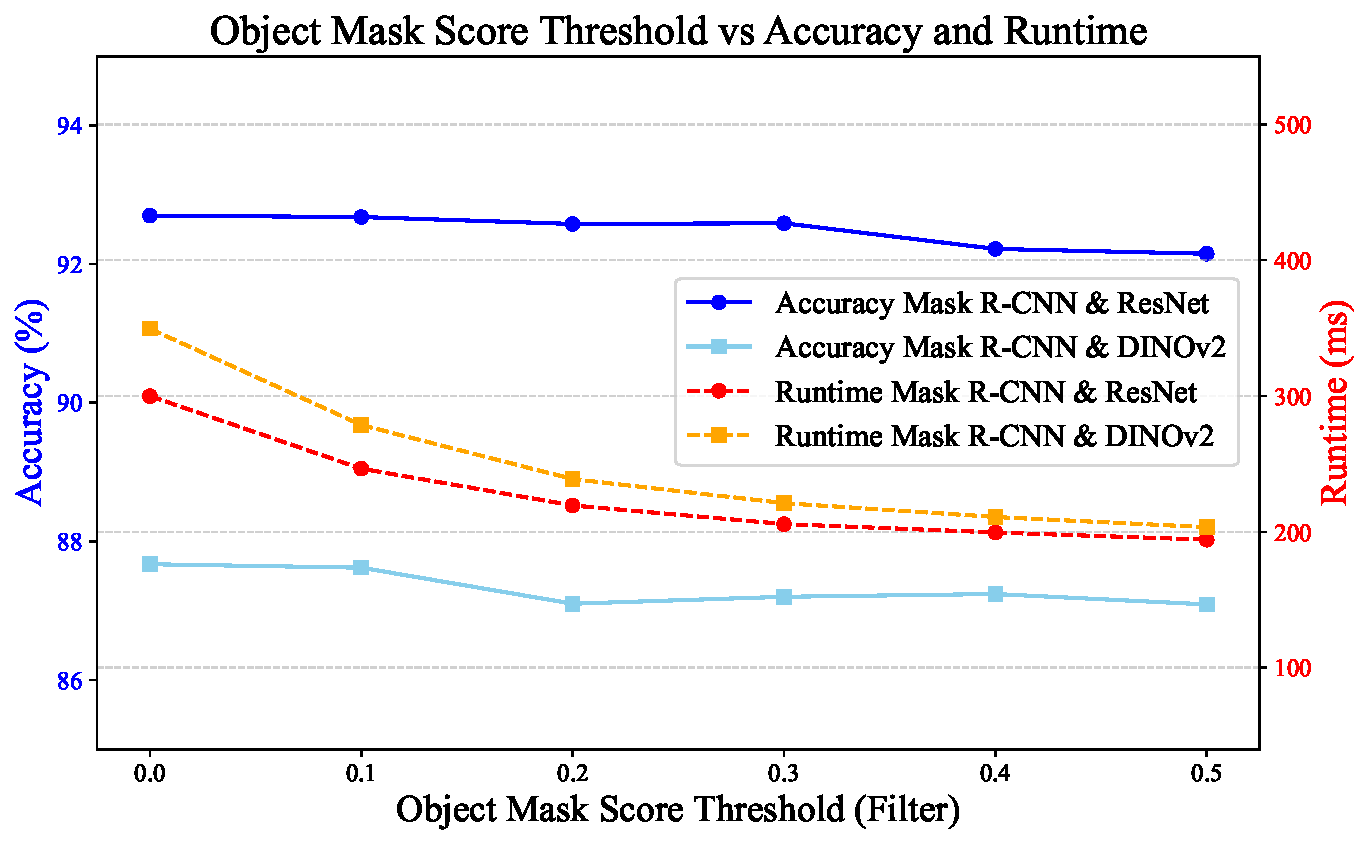
\includegraphics[width=\columnwidth]{runtime.pdf}
    \caption{As the object mask score threshold increases, AirRoom's performance experiences a slight decline; however, the efficiency improves significantly.}
    \label{fig:runtime}
\end{figure}

\begin{table}[ht]
\centering
\begin{tabular}{l|cc}
\toprule
\multirow{2}{*}{\textbf{Modules}} & \multicolumn{2}{c}{\textbf{Runtime (ms)}} \\
 & ResNet & DINOv2 \\
\midrule
Global Feature Extractor & 42.5 & 56.2 \\
Global Retrieval & 0.1 & 0.1 \\
Instance Segmentation & 352.6 & 343.2 \\
Receptive Field Expander & 0.7 & 0.6 \\
Object Feature Extractor & 51.1 & 66.6 \\
Object-Aware Scoring & 2.2 & 2.1 \\
Fine-Grained Retrieval & 87.8 & 87.4 \\
\midrule
\textbf{Total} & \textbf{538.5} & \textbf{557.6} \\
\bottomrule
\end{tabular}%
\caption{Semantic-SAM \& ResNet / DINOv2 Runtime.}
\label{tab:module_runtime_ssam}
\end{table}

\begin{table}[ht]
\centering
\begin{tabular}{l|c|c}
\toprule
\textbf{Methods} & \textbf{Runtime (ms)} & \textbf{Accuracy (\%)}\\
\midrule
CVNet & 111.3 & 11.71 \\
DINOv2 & \textbf{16.7} & 53.91 \\
Patch-NetVLAD & 100.5 & 64.86 \\
AnyLoc & 45.5 & 89.69 \\
\rowcolor{Lavender} AirRoom & 194.2 & \textbf{92.15} \\
\bottomrule
\end{tabular}
\caption{Runtime Comparison with State-of-the-Art Methods.}
\label{tab:runtime_comparison}
\end{table}

When Mask R-CNN is used for instance segmentation, \tref{tab:module_runtime_mr} demonstrates that increasing the object mask score threshold significantly reduces the runtime of the Object Feature Extractor when ResNet is employed. This is attributed to the reduced number of objects and patches requiring processing. A similar trend is observed with DINOv2 as the Object Feature Extractor, as shown in \tref{tab:module_runtime_md}. Additionally, \tref{tab:module_accuracy} indicates that AirRoom's performance remains largely unaffected by the rise in the object mask score threshold, regardless of the chosen Object Feature Extractor. This observation is further illustrated in \fref{fig:runtime}. However, when Semantic-SAM is used for instance segmentation, AirRoom faces efficiency challenges due to Semantic-SAM's significantly slower performance, as detailed in \tref{tab:module_runtime_ssam}.

\tref{tab:runtime_comparison} compares runtime across methods. AirRoom requires 80ms more than CVNet but achieves over 80\% performance improvement. Compared to Patch-NetVLAD, AirRoom's runtime is approximately double, with a performance gain exceeding 30\%. While DINOv2 completes tasks in 10–20ms, AirRoom adds 170ms and improves performance by over 40\%. Relative to AnyLoc, AirRoom increases runtime by just over 150ms but captures an additional 20\% of the remaining performance potential. These results demonstrate that AirRoom delivers significant performance gains even within limited improvement margins, underscoring its effectiveness despite incremental runtime.

Currently, AirRoom allocates approximately 90ms to Fine-Grained Retrieval, utilizing LightGlue for feature matching. Exploring more lightweight and faster alternatives could further enhance efficiency. In real-world applications such as Real-Time Navigation, room reidentification times between 50–200ms are generally acceptable, with accuracy as the primary concern. While AirRoom is slightly slower than some baselines, it achieves substantial accuracy improvements, effectively balancing runtime and performance. This makes AirRoom well-suited for practical scenarios, meeting real-world runtime requirements while maintaining high reliability and precision.

\end{document}
